\section{Linear parameter estimation} 
\label{LinParamEst}

%As can be seen in \eqref{multistate model_smallsignal}, the small signal model of such a multi-state/ multi-input system consists of two Jacobian matrices, one for the states and one for the inputs to the system. It should be emphasized however that these matrices have to be evaluated at the operating points, at $(\bar{x}, \bar{u})$. It is a reasonable statement since the inputs to the model are the small signal values of OD and differential pressures, dp, from the pumps. Therefore the same excitation to the real test setup can be carried out by taking the operating values into account and by adding them to the small signal values. 

The method that describes the linear parameter estimation is shown in \figref{fig:parame_block_lin} below:

\begin{figure}[H]
\centering
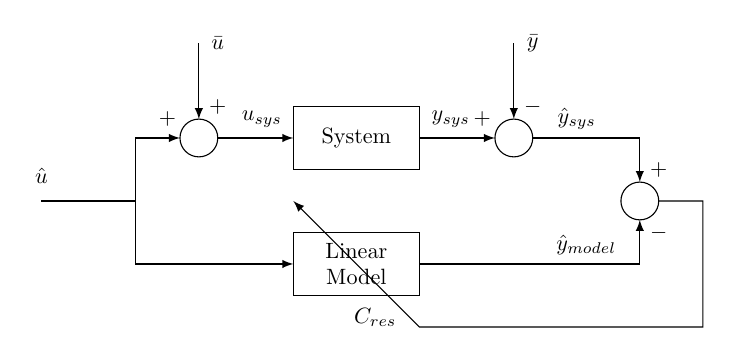
\begin{tikzpicture} [scale=0.8,transform shape]

\draw  (3,-1.5) rectangle (5,-2.5);
\node at (4,-1.8) {Linear};
\node at (4,-2.2) {Model};

\draw  (3,0.5) rectangle (5,-0.5);
\node at (4,0) {System};

\node at (8.8,-1.5) {$-$};
\node at (5.5,0.3) {$y_{sys}$};
\node at (7.5,0.3) {$\hat{y}_{sys}$};
\node at (7.65,-1.7) {$\hat{y}_{model}$};
\node at (4.3,-2.85) {$C_{res}$};
\node at (-1,-0.6) {$\hat{u}$};
\node at (1.8,1.5) {$\bar{u}$};
\node at (2.5,0.3) {$u_{sys}$};
\node at (8.8,-0.5) {$+$};
\node at (1.8,0.5) {$+$};
\node at (6,0.3) {$+$};
\node at (6.8,0.5) {$-$};
\node at (1,0.3) {$+$};
\node at (6.8,1.5) {$\bar{y}$};

\draw  (8.5,-1) ellipse (0.3 and 0.3);
\draw  (6.5,0) ellipse (0.3 and 0.3);
\draw  (1.5,0) ellipse (0.3 and 0.3);

\draw [-latex](5,0) -- (6.2,0);

\draw [-latex](0.5,-1) -- (0.5,0) -- (1.2,0);
\draw [-latex](0.5,-1) -- (0.5,-2) -- (3,-2);
\draw (-1,-1) -- (0.5,-1);
\draw [-latex](5,-2) -- (8.5,-2) -- (8.5,-1.3);
\draw [-latex](8.8,-1) -- (9.5,-1) -- (9.5,-3) -- (5,-3) -- (3,-1);

\draw [-latex](1.8,0) -- (3,0);
\draw [-latex](1.5,1.5) -- (1.5,0.3);
\draw [-latex](6.5,1.5) -- (6.5,0.3);
\draw [-latex](6.8,0) -- (8.5,0) -- (8.5,-0.7);
\end{tikzpicture}% 
\caption{Parameter identification block diagram for the linear system. }
\label{fig:parame_block_lin}
\end{figure}

In this case small-signal inputs are applied to both the test setup and the model.  Now the linearized model is compared to the real system, therefore the operating point is taken into account. Since the linear model is only valid for small deviations around the operating point, the real system has to be excited around the same operating point to obtain identical behavior. In order to achieve it, the operating values are added to both the input and the output such as: 

\begin{equation}
u_{sys} = \bar{u} + \hat{u}
 \label{u_smallsignal}
\end{equation}

\begin{minipage}[t]{0.20\textwidth}
Where\\
\hspace*{8mm} $\hat{u}$ \\
\hspace*{8mm} $\bar{u}$ \\
\hspace*{8mm} $u_{sys}$ 
\end{minipage}
\begin{minipage}[t]{0.68\textwidth}
\vspace*{2mm}
is the small-signal input, \\
is the operating value of the input,\\
is the input to the real-life system. 
\end{minipage}
\begin{minipage}[t]{0.10\textwidth}
\vspace*{2mm}
\textcolor{White}{te}$\unit{bar}$
\textcolor{White}{te}$\unit{bar}$
\textcolor{White}{te}$\unit{bar}$
\end{minipage} 

\begin{equation}
  y_{sys} = \bar{y} + \hat{y}_{sys} 
 \label{u_smallsignal}
\end{equation}

\begin{minipage}[t]{0.20\textwidth}
Where\\
\hspace*{8mm} $\hat{y}_{sys}$ \\
\hspace*{8mm} $\bar{u}_{sys}$ \\
\hspace*{8mm} $y_{sys}$ 
\end{minipage}
\begin{minipage}[t]{0.68\textwidth}
\vspace*{2mm}
is the small-signal output from the real-life system, \\
is the operating value of the output,\\
is the output from the real-life system. 
\end{minipage}
\begin{minipage}[t]{0.10\textwidth}
\vspace*{2mm}
\textcolor{White}{te}$\unit{bar}$
\textcolor{White}{te}$\unit{bar}$
\textcolor{White}{te}$\unit{bar}$
\end{minipage} 

During the linear parameter estimation, the same problem is solved as it is shown in \eqref{ObjectiveFunction}. In this case, however, the parameters are varied according to the comparison of the small-signal outputs.  

\subsection{Model Parameters}
\label{estimateParameters}
In order to obtain a complete model of the physical setup, all the parameters describing the components have to be defined. In \secref{SubSecEstimation} a detailed
description of the known parameters of the system has been done. Nevertheless, in the linearized state-space model more parameters have to be indentified
due to the introduction of the operating points values. Hence, in the current chapter a detailed compilation of the unknown parameters of the physical water distribution setup is carried out.


\textbf{Unknown Parameters}
The unknown parameters are the ones related with the form losses, $k_f$, and form friction ,$f$, of the pipes. Despite they are 
provided by the manufactures they need to be estimated. On one hand, the form losses depend on the fittings and bends of the pipes which are not always known. 
On the other hand, the friction losses depend on the inside average roughness of the pipes, $\epsilon$, which can change its value due to passage of time 
and rust generated inside pipes or fittings. 

%The friction and form losses are part of the model of a pipe, and are given by the following equation
%
%\begin{equation}
%  \lambda (q) =  \frac{8fL}{\pi^{2}gD^5} \rho g  |q| q + k_f \frac{8}{\pi^2gD^4} \rho g |q| q
%  \label{frictionestimation}
%\end{equation}

%From the above equation it can be seen that either estimating only for $k_f$ or $f$ will have the same result in the value of $\lambda (q)$.
%Therefore, it has been decided to carry out the estimation of the total value of $\lambda (q)$, hence discarding the respective values of $k_f$ and $f$.

Furthermore, the operating points of the flow through the chords, $\pmb{\bar{z}}$, is also unknown. These values, which correspond to the $8$ flow chords, are introduced in the linearized expression of both pipes 
and valves, see \eqref{lambda_lin} and \eqref{mu_lin}. Thus, not only pipe parameters introduce uncertainties into the system model but also the lack of knowledge of the chord operating points.

Consequently, it has been decided to estimate the total expression for the pressure across the pipes and valves in order to reduce the amount of unknowns in the system.

The system has $15$ pipes in total,  from \eqref{lambda_lin} it can be seen that either tunning for $k_f$, $f$ or $\pmb{\bar{z}}$ it will have the same result for the total
value of the pressure across the pipes, $\lambda(\pmb{{B_1^{T}}}\pmb{z})$. For this reason the pressure across the 15 pipes is estimated.

The linearized valve expression, see \eqref{mu_lin}, consists of the term depending on the chord flows and the one depending on the $OD$. Both terms include the operating 
point of the chord flows inside them, thus, the pressure difference given by both terms has to be estimated. In the system 4 valves take part, 
resulting in 8 unknowns in total. 

The WT connection edge, see \eqref{gamma_lin}, is conformed by two valves and one pump. Although the parameters corresponding to the pump are considered as known, the ones 
corresponding to the valves have to be estimated. Resulting in two more unknowns for the system. 

All in all, the system has $24$ unknown terms which will be calculated following the estimation process described in the next section.
\subsection{Measurements on the test setup}
\label{LinParamEst_measurements}

In order to verify the state-space model derived in \chapref{LinParamEst} with the physical setup, an estimation for the parameters defined in \secref{estimateParameters}
is carried out.

From the system setup, $9$ different relative pressures can be measured, following \figref{systemdiagram} notation the sensors are placed in: 
$n_2$ $n_4$ $n_5$ $n_7$ $n_{10}$ $n_{11}$ $n_{15}$ $n_{16}$ $n_{18}$. However, the estimation will be done only regarding the four PMA relative pressure 
sensors across the end-users and the pressure in the WT, since those are the outputs that will be controlled in \secref{SystemLin_control}. Thus, the estimation will only focus on obtaining the best fit for those sensor outputs relevant in the control part. 

The relationship between pressures, where DpCXX describes the pressure difference for the XX component, is obtained in the same way as \secref{SubSecEstimation} and can be defined as:

\text{\underline{Node 10}}
\vspace{4mm}
\begin {equation}
     y_1 = DpC20 + DpC21  
\end{equation}

\text{\underline{Node 11}}
\vspace{4mm}
\begin {equation}
     y_2 = DpC24
\end{equation}


\text{\underline{Node 15}}
\vspace{4mm}
\begin {equation}
     y_3 = DpC28 + DpC20 
\end{equation}

\text{\underline{Node 15}}
\vspace{4mm}
\begin {equation}
     y_4 = DpC31 
\end{equation}

There is no need to define a relation with a referent point for the WT node, since the pressure across the WT is the state of the state-space model. 

\subsection{Linear Estimation Outcomes}
In \appref{LinResults} the results of the estimation process are shown, where the $24$ terms defining the pressure across the unknowns edges are estimated.
From the tests it can be seen a slightly different behavior between the model and the data from the setup, especially at time $t = 350s$. This dissimilar 
behavior showing up at some time samples could make the model unsuitable for the real setup, thus making it incorrect to be used in a model based control scheme. 

In light of the above considerations, a different approach for the parameter estimation is attempted. In \secref{estimateParameters} it has been described how the 
unknown pressures across the edges are estimated in order to build up the state-space matrices of the system. Nonetheless, as the estimation did not 
succeed it has been decided to estimate the final values of the state-space matrices stated in \eqref{statespace_4} and \eqref{outputfinaleq}. 
Altogether these matrices sum up to 44 unknown parameters, which are the ones to be estimated. The outputs to be compared with the test setup remain 
the same as in \secref{LinParamEst_measurements}, as well as the toolbox used for estimating.

\textbf{Estimation Data}

As the parameter estimation is based on a linearized model an operating point for the system is chosen. This point is based on the WT being approximately half way full which allows for an equal amount of deviation in both directions. For the chosen operating point, data is gather from the system while small steps are individually applied to the two main pumps and the opening degree of the PMA valves. In order to use the data for parameter estimation the operating point is subtracted, leaving only small signal values.  

The operating point of the PMA valves is placed at $70\%$ opening corresponding to $63^{\circ}$ and the small signal values for the estimation can be seen in \figref{fig:est_OD_data_final}.

\begin{figure}[H]
\centering
% This file was created by matlab2tikz.
%
%The latest updates can be retrieved from
%  http://www.mathworks.com/matlabcentral/fileexchange/22022-matlab2tikz-matlab2tikz
%where you can also make suggestions and rate matlab2tikz.
%
\definecolor{mycolor1}{rgb}{0.00000,0.44700,0.74100}%
\definecolor{mycolor2}{rgb}{0.85000,0.32500,0.09800}%
\definecolor{mycolor3}{rgb}{0.92900,0.69400,0.12500}%
\definecolor{mycolor4}{rgb}{0.49400,0.18400,0.55600}%
%
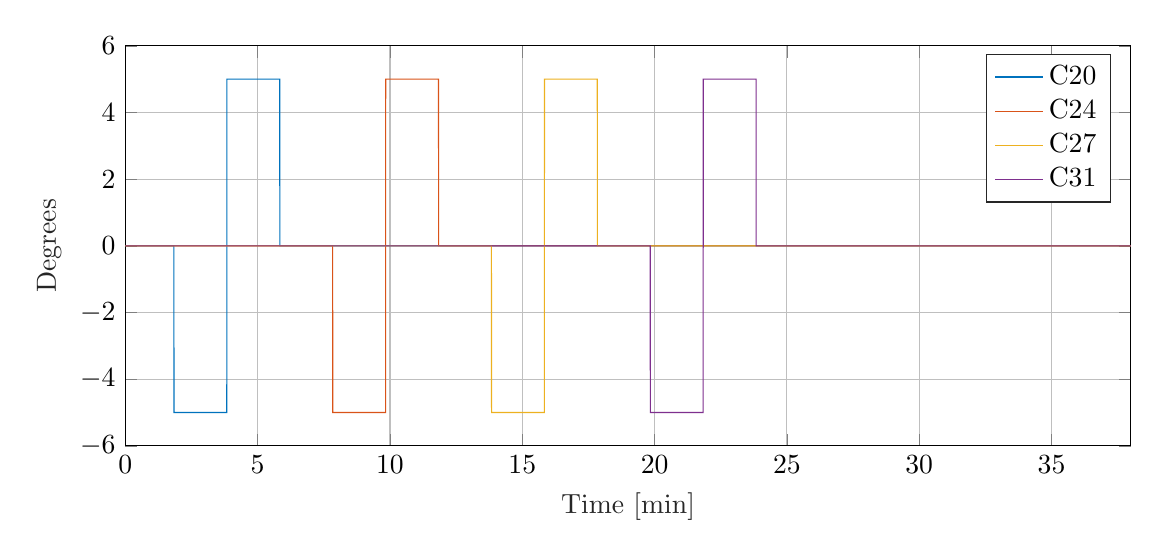
\begin{tikzpicture}

\begin{axis}[%
width=5.028in,
height=2in,
at={(0.758in,0.481in)},
scale only axis,
xmin=0,
xmax=38,
xlabel style={font=\color{white!15!black}},
xlabel={Time [min]},
ymin=-6,
ymax=6,
ylabel style={font=\color{white!15!black}},
ylabel={Degrees},
axis background/.style={fill=white},
%title style={font=\bfseries},
%title={Valve opening degree},
xmajorgrids,
ymajorgrids,
legend style={legend cell align=left, align=left, draw=white!15!black}
]
\addplot [color=mycolor1]
  table[row sep=crcr]{%
0	-4.00248723053664e-11\\
1.83416666666667	-4.00248723053664e-11\\
1.83916666666666	-5.00000000004003\\
3.83416666666667	-5.00000000004003\\
3.83916666666666	4.99999999995997\\
5.83416666666667	4.99999999995997\\
5.83916666666667	-4.00248723053664e-11\\
53.3325	-4.00248723053664e-11\\
};
\addlegendentry{C20}

\addplot [color=mycolor2]
  table[row sep=crcr]{%
0	-4.4146020172775e-11\\
7.83416666666667	-4.4146020172775e-11\\
7.83916666666667	-5.00000000004415\\
9.83416666666667	-5.00000000004415\\
9.83916666666667	4.99999999995585\\
11.8341666666667	4.99999999995585\\
11.8391666666667	-4.4146020172775e-11\\
53.3325	-4.4146020172775e-11\\
};
\addlegendentry{C24}

\addplot [color=mycolor3]
  table[row sep=crcr]{%
0	-4.74145167572715e-11\\
13.8341666666667	-4.74145167572715e-11\\
13.8391666666667	-5.00000000004742\\
15.8341666666667	-5.00000000004742\\
15.8391666666667	4.99999999995258\\
17.8341666666667	4.99999999995258\\
17.8391666666667	-4.74145167572715e-11\\
53.3325	-4.74145167572715e-11\\
};
\addlegendentry{C27}

\addplot [color=mycolor4]
  table[row sep=crcr]{%
0	-4.05933064939745e-11\\
19.8341666666667	-4.05933064939745e-11\\
19.8391666666667	-5.00000000004059\\
21.8341666666667	-5.00000000004059\\
21.8391666666667	4.99999999995941\\
23.8341666666667	4.99999999995941\\
23.8391666666667	-4.05933064939745e-11\\
53.3325	-4.05933064939745e-11\\
};
\addlegendentry{C31}

\end{axis}
\end{tikzpicture}% 
\caption{Small signal values of the opening degrees of the pma valves.}
\label{fig:est_OD_data_final}
\end{figure}

To acheive a 50\% fill level of the WT in stady state combined with the chosen operating point of the valves, the operating point of the pumps has to be set at a differential pressure of $\Delta _p = 0.2 Bar$. The required operating point is found by experimental tests made on the setup, the small signal values used in the estimation are shown in \figref{fig:est_deltap_data_final}. 

\begin{figure}[H]
\centering
% This file was created by matlab2tikz.
%
%The latest updates can be retrieved from
%  http://www.mathworks.com/matlabcentral/fileexchange/22022-matlab2tikz-matlab2tikz
%where you can also make suggestions and rate matlab2tikz.
%
\definecolor{mycolor1}{rgb}{0.00000,0.44700,0.74100}%
\definecolor{mycolor2}{rgb}{0.85000,0.32500,0.09800}%
%
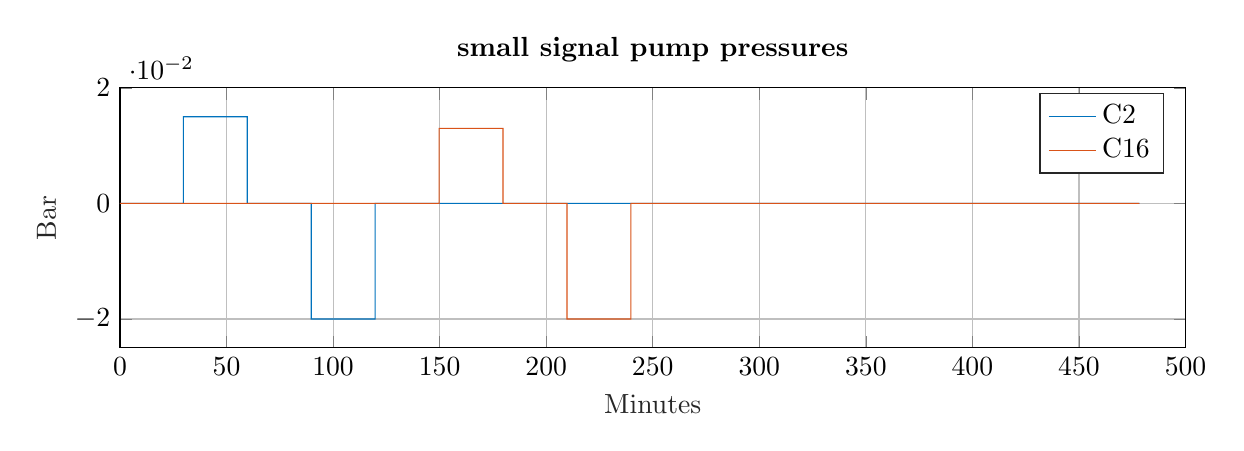
\begin{tikzpicture}

\begin{axis}[%
width=5.328in,
height=1.3in,
at={(1.011in,0.642in)},
scale only axis,
xmin=0,
xmax=500,
xlabel style={font=\color{white!15!black}},
xlabel={Minutes},
ymin=-0.025,
ymax=0.02,
ylabel style={font=\color{white!15!black}},
ylabel={Bar},
axis background/.style={fill=white},
title style={font=\bfseries},
title={small signal pump pressures},
xmajorgrids,
ymajorgrids,
legend style={legend cell align=left, align=left, draw=white!15!black}
]
\addplot [color=mycolor1]
  table[row sep=crcr]{%
0	-0\\
29.7508333333333	-0\\
29.7516666666667	0.0149999999999864\\
59.7508333333333	0.0149999999999864\\
59.7516666666667	-0\\
89.7508333333333	-0\\
89.7516666666667	-0.0200000000000387\\
119.750833333333	-0.0200000000000387\\
119.751666666667	-0\\
478.333333333333	-0\\
};
\addlegendentry{C2}

\addplot [color=mycolor2]
  table[row sep=crcr]{%
0	-0\\
149.750833333333	-0\\
149.751666666667	0.0129999999999768\\
179.750833333333	0.0129999999999768\\
179.751666666667	-0\\
209.750833333333	-0\\
209.751666666667	-0.0200000000000387\\
239.750833333333	-0.0200000000000387\\
239.751666666667	-0\\
478.333333333333	-0\\
};
\addlegendentry{C16}

\end{axis}
\end{tikzpicture}% 
\caption{Small signal values of the differential pressure of the two main pumps.}
\label{fig:est_deltap_data_final}
\end{figure}



\textbf{Estimation Result}

The following figures show the comparison between the data obtained from the lab and the outputs of the model with the estimated parameters.  

\begin{figure}[H]
  \centering
    % This file was created by matlab2tikz.
%
%The latest updates can be retrieved from
%  http://www.mathworks.com/matlabcentral/fileexchange/22022-matlab2tikz-matlab2tikz
%where you can also make suggestions and rate matlab2tikz.
%
\definecolor{mycolor1}{rgb}{0.00000,0.44700,0.74100}%
\definecolor{mycolor2}{rgb}{0.85000,0.32500,0.09800}%
%
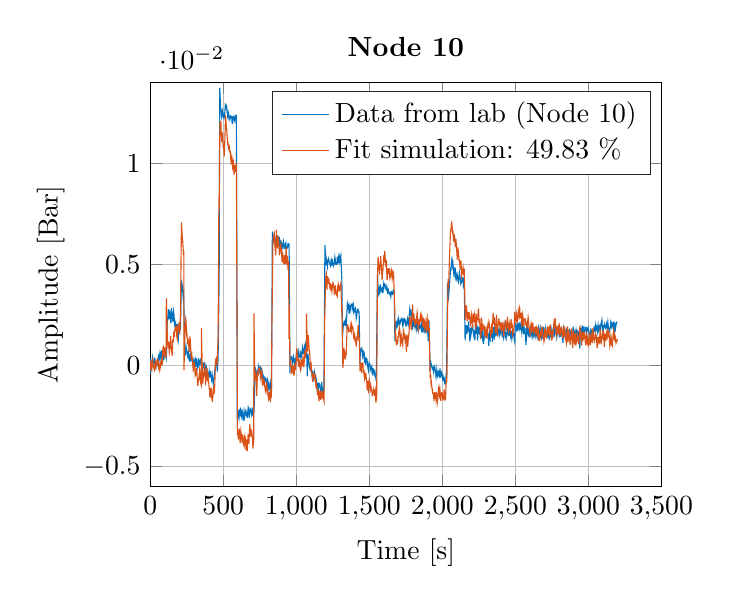
\begin{tikzpicture}

\begin{axis}[%
width=2.5556in,
height=2.02135in,
at={(1.011in,0.642in)},
scale only axis,
xmin=0,
xmax=3500,
xlabel={Time [s]},
xmajorgrids,
ymin=-0.006,
ymax=0.014,
ylabel={Amplitude [Bar]},
ymajorgrids,
axis background/.style={fill=white},
title style={font=\bfseries},
title={Node 10},
legend style={legend cell align=left,align=left,draw=white!15!black}
]
\addplot [color=mycolor1,solid]
  table[row sep=crcr]{%
0.05	-0.000410544037145466\\
0.45	0.000346347458455742\\
7.45	-6.08079667644423e-05\\
14.7	0.000331557624632661\\
15.9	0.000392456940371017\\
17.8	0.000228028787879669\\
26.4	6.18606549359912e-05\\
28.9	0.000362877272727213\\
31.45	0.000355917350929741\\
36.05	9.84002443785159e-05\\
39	-6.77678885624144e-05\\
44.15	0.000195839149557453\\
46.95	0.00018191930595754\\
51	-1.8178445749889e-05\\
51.7	8.36104105559898e-05\\
55.95	0.000429866520034905\\
60.25	0.000261958406643781\\
65.95	0.000589074731181388\\
68.8	0.000393326930593269\\
73.8	0.000663893890515216\\
76.15	0.000686513636360853\\
79.9	0.00025847844574442\\
83.15	0.000292408064511973\\
85.25	0.000533395356788868\\
90.35	0.000362877272727213\\
95	0.000716963294229767\\
97.4	0.000482935923748734\\
102.35	0.000686513636356578\\
103.75	0.000638664173985198\\
109.9	0.000372447165201406\\
110.65	0.000458576197458233\\
117.6	0.00241953416422269\\
119.7	0.00222987629520835\\
124.95	0.00278232008797666\\
125.4	0.00274491050830653\\
128.5	0.0023003455034179\\
133.6	0.00272229076245842\\
140.15	0.00218115684261738\\
141.5	0.00208284794721442\\
145.8	0.00284234941348635\\
147.55	0.00267357130986176\\
154.85	0.00218376681328825\\
155.25	0.00216114706744086\\
159.75	0.00267531129032156\\
162.65	0.00252915293255573\\
167.5	0.00195147942325852\\
170.9	0.00187927023460766\\
172.35	0.00212721744868893\\
177.05	0.00202455860214534\\
181.95	0.0016243630987241\\
186.9	0.00204282839687486\\
191.75	0.00128419692082607\\
191.9	0.00127723699902665\\
196.5	0.00188275019550807\\
199.25	0.00167743250244859\\
204.15	0.00213765733138238\\
206.5	0.00173050190616597\\
213.6	0.00415081471161763\\
215.05	0.00417256446724401\\
220.05	0.00380455860212128\\
221.25	0.00383326827954425\\
224.55	0.00344699261971904\\
228.65	0.00358358108502591\\
236	0.000876171505402173\\
238.15	0.000459446187706242\\
245.4	0.000932720870019971\\
250.75	0.000625614320644341\\
255.25	0.000476845992217589\\
258.15	0.000658673949196553\\
260.05	0.000703043450656138\\
264.7	0.00030980786903434\\
269.25	0.00024716857283813\\
272.75	0.000530785386128274\\
274	0.000636054203342035\\
278.5	0.000305457917903651\\
283.05	0.000410726735120243\\
287.65	0.000200189100678538\\
289.9	0.000255868475073889\\
290.5	0.000128849902247957\\
295.3	0.000235858699920821\\
298.55	3.40209677589243e-05\\
306.6	0.000315027810368962\\
309.45	9.75302541619261e-05\\
311.8	-6.95078690128026e-05\\
316.8	0.000333297605105587\\
317.65	0.000332427614883168\\
323.2	-8.34277126102179e-05\\
328.35	0.000141899755615849\\
330.2	-9.90875366638777e-05\\
331.95	-8.60855328135846e-06\\
334.95	0.000241948631482164\\
340.2	8.62203812233009e-05\\
346.35	0.000312417839707341\\
348.65	0.000346347458469204\\
353.8	-0.000693290860219464\\
355.5	-0.000789859775186086\\
360.5	3.05410068577872e-05\\
361.35	-0.000163466813276558\\
362.95	8.27404203520288e-05\\
369.8	0.000134069843591128\\
373.45	-0.000303535239501634\\
376.1	-0.00018173660802312\\
380.8	1.14012219001314e-05\\
383.8	-7.29878299124964e-05\\
390.85	-0.000349644721428843\\
393.6	-0.000344424780075708\\
398.15	-0.000571492228759435\\
403.15	-0.000320935044004433\\
405.2	-0.000570622238534157\\
407.3	-0.000569752248311711\\
412.35	-0.000266125659832944\\
412.95	-0.000436643743910226\\
419.9	-0.000712430645124523\\
424.1	-0.000454913538619844\\
427.7	-0.000675891055693906\\
431.3	-0.00091252839682876\\
435.1	-0.000716780596265149\\
442.45	-0.00027221559137014\\
442.95	-0.000303535239483149\\
446.6	8.97003420917697e-05\\
453.5	0.000147119696974646\\
457.05	-9.82175464130375e-05\\
459.45	-0.000299185288339693\\
464.6	0.000348957429129437\\
471.95	0.00423694374386946\\
475.95	0.013733757038115\\
481.45	0.0128237472629323\\
486.45	0.0124087619257168\\
487.8	0.0123121930107417\\
494.05	0.0126097296676435\\
494.1	0.0126079896871929\\
499.15	0.012275653421331\\
504.75	0.0122243239980762\\
505.35	0.0124070219452776\\
508.8	0.0123574325024678\\
514.8	0.0129342360214779\\
517.1	0.0129159662267669\\
523.35	0.0126732389540664\\
524.3	0.0127132585043953\\
530.15	0.0123504725806428\\
534.45	0.0124931509774897\\
537.1	0.0123269828445857\\
538.3	0.0123931021016816\\
545.3	0.0121590747311743\\
545.7	0.0121721245845507\\
550.45	0.0123496025904175\\
557.6	0.0123174129521076\\
560.45	0.0120268362170109\\
561.45	0.0119494070869948\\
566.05	0.0123061030791732\\
568.2	0.0123226328934564\\
574.8	0.0121068753176971\\
575.3	0.012137324975565\\
580.95	0.0123565625122027\\
583.65	0.012371352346024\\
585.9	0.0121442848973502\\
589.95	0.0122443337732179\\
596.4	-0.00311447365592835\\
597.65	-0.00260639936461893\\
602.8	-0.00233496241449552\\
608.2	-0.00257333973608093\\
611.1	-0.0022888529325612\\
614.55	-0.00238716182796703\\
618.8	-0.00216183435973244\\
619.55	-0.00217749418378185\\
623.55	-0.00252114032260375\\
628.6	-0.00230886270774841\\
633.35	-0.00254898000977868\\
635.85	-0.00235410219942048\\
641.5	-0.00270731823069206\\
642.4	-0.00270992820137075\\
647.7	-0.00230973269794527\\
649.9	-0.00243675127080245\\
654.85	-0.00226101324535499\\
656.85	-0.00231669261974754\\
663.65	-0.002581169648117\\
663.85	-0.00260204941351527\\
668.8	-0.00221403377320961\\
671.9	-0.00237759193551165\\
675.1	-0.00217053426197958\\
680.1	-0.00245154110463797\\
685.8	-0.00215661441838358\\
688.2	-0.00212964472139129\\
692.6	-0.00233061246334637\\
694.95	-0.00244284120235672\\
700.1	-0.00221055381233123\\
703.25	-0.00236193211146224\\
705.85	-0.00222447365592154\\
711.05	-0.00227667306938736\\
715.25	-0.000969947751708777\\
718.1	-6.08079667656636e-05\\
723.85	-0.000624561632476123\\
727.9	-0.000392274242427909\\
731	-0.000570622238477314\\
735.45	-0.00029483533724739\\
741.4	-6.25479472133872e-05\\
744.75	-0.000443603665705394\\
744.85	-0.000452303567955364\\
748.5	-6.68978983568436e-05\\
755.8	-7.55978005812508e-05\\
759	-0.000536692619728218\\
761	-0.000573232209184427\\
764	-0.000253945796653388\\
767.95	-0.000353994672504077\\
773.35	-0.000716780596276528\\
776.8	-0.000596721945235801\\
781.65	-0.000902088514150939\\
781.8	-0.000916878347977906\\
786.75	-0.000605421847502841\\
793.15	-0.000671541104573181\\
796.25	-0.000905568475043528\\
798.25	-0.00105781676439415\\
802.25	-0.00076898000974801\\
803.75	-0.000865548924694731\\
807.8	-0.00114916573797497\\
812.85	-0.000864678934517776\\
818.5	-0.00113611588463836\\
820	-0.00126922438902988\\
825	-0.000889908651005494\\
829.95	-0.00120745508306891\\
833.25	0.00253002292275972\\
836.15	0.00662593690126279\\
840.9	0.00639190953076116\\
847.75	0.00607697306934232\\
848	0.00609089291293549\\
851.4	0.00643279907133523\\
855.6	0.00627185087976023\\
859.05	0.00592994472134911\\
864.3	0.00597779418369418\\
869.1	0.00643105909091879\\
870.1	0.00631361041053971\\
874.6	0.00610394276634885\\
879.6	0.00625706104589632\\
883.4	0.00603782350914775\\
885.9	0.00618311187675863\\
890.75	0.0058733953566375\\
893.2	0.00603695351888836\\
896.4	0.00590558499504118\\
900.65	0.00605435332346793\\
906.3	0.00582815586509333\\
907.7	0.00580640610943853\\
912.7	0.00611873260017864\\
914.35	0.0060430434505904\\
917.9	0.00587078538604124\\
922.9	0.00596648431073141\\
924	0.00574376681319541\\
929.6	0.00599867394911235\\
932.7	0.00578117639291667\\
940.8	0.00581858597262089\\
942.85	0.00602999359723391\\
950.9	0.00600650386121948\\
951.2	0.00582293592376437\\
956.5	-0.000392274242405177\\
958.6	0.00017930933528737\\
961.55	0.000415946676507462\\
968	0.000439436412573047\\
973.15	9.6660263908227e-05\\
973.35	0.000102750195479534\\
980.7	0.000415076686293564\\
987.05	7.31705279279071e-05\\
992.65	0.000374187145705251\\
994.9	0.000108840127084925\\
995.7	8.53503909909181e-05\\
1002.8	0.000762202785993843\\
1003.05	0.000823102101723872\\
1009.7	0.00045770620729263\\
1011.4	0.000404636803590153\\
1017.1	0.00070130347024111\\
1017.55	0.000669983822176395\\
1020.2	0.000429866520043787\\
1027.1	0.000384627028414353\\
1030.1	0.000607344526035614\\
1034.75	0.000454226246442646\\
1039.7	0.000728273167276028\\
1042.05	0.00087182155436813\\
1046.35	0.000569934946314327\\
1047.1	0.000569934946314327\\
1053.7	0.000850071798662144\\
1056.45	0.00067172380262695\\
1060.5	0.000964040518185577\\
1061.8	0.000910101124178248\\
1066.75	0.00111889877806426\\
1069.6	0.000945770723352335\\
1075.75	-0.00053930259044388\\
1076.55	-0.0001399770772266\\
1080.4	0.000569064956043586\\
1083.95	0.000275008260057108\\
1091.25	-0.000121707282501354\\
1093.95	-0.000186956549340728\\
1096.35	1.92311339376472e-05\\
1098.85	-2.07884164594718e-05\\
1106.05	-0.000398364174010568\\
1109	-0.000556702394892694\\
1112.45	-0.000347034750747294\\
1113.7	-0.000374874437979095\\
1118.5	-0.000621081671569296\\
1123.35	-0.000316585092919236\\
1128.15	-0.000574972189657741\\
1128.85	-0.000562792326515127\\
1132.65	-0.000770719990266788\\
1135.75	-0.000635001515156774\\
1142.75	-0.000998657429052169\\
1144.25	-0.000862068963762341\\
1149.25	-0.00120832507325441\\
1150.45	-0.00118744530788739\\
1154.25	-0.000880338758521698\\
1160.15	-0.000925578250196624\\
1165.05	-0.00126226446717079\\
1168.55	-0.00136231334294756\\
1172.4	-0.000993437487728899\\
1174.25	-0.00081856945256642\\
1179.25	-0.00130663396865452\\
1180	-0.00109087639287531\\
1184.75	-0.00136318333328656\\
1189.2	-0.00131794384164005\\
1194.55	0.00422128391986554\\
1196.15	0.00595604442814737\\
1205.75	0.00495207570865411\\
1207.25	0.00518262311824039\\
1213	0.00491466612908062\\
1214.85	0.00518175312807193\\
1221.05	0.00529398186708796\\
1223.15	0.0051252037635138\\
1224	0.00521829271756225\\
1226.05	0.00508344423275139\\
1234.2	0.00493119594330416\\
1238.65	0.00520785283475084\\
1239	0.00522003269788776\\
1244.2	0.00494163582599619\\
1246.75	0.00526005224830192\\
1251.75	0.00496947551319385\\
1255.1	0.00491640610950844\\
1260.9	0.00509214413490758\\
1264.55	0.00536184110459181\\
1268.25	0.00517653318667477\\
1269.05	0.0050042751221995\\
1278.45	0.00500775508310061\\
1281.2	0.00538359086024662\\
1285.55	0.00505560454549117\\
1288.85	0.00533748137824411\\
1293.55	0.00512955371463455\\
1297.2	0.00536184110458043\\
1300.3	0.00520959281522984\\
1305.1	0.00541491050832268\\
1312.5	0.00417952438911448\\
1316.55	0.00142339535678251\\
1321.3	0.00189406006834225\\
1327.1	0.00216636700881032\\
1331	0.00219072673505002\\
1333.15	0.00199497893441822\\
1335.4	0.00199323895400175\\
1338.05	0.00219159672528668\\
1342.4	0.00199236896369689\\
1349.35	0.00300416759535416\\
1351.1	0.00306506691111827\\
1353.1	0.00278319007829714\\
1356.8	0.003048537096872\\
1361.6	0.00255003269798953\\
1364.2	0.00272142077231344\\
1367.65	0.00294674824055938\\
1372.6	0.00275970034220313\\
1373.7	0.00294413826990628\\
1381.55	0.00304592712623025\\
1385.7	0.00282581959938147\\
1390.5	0.00299024775188036\\
1392.3	0.00275970034227704\\
1393.6	0.00280058988281418\\
1395.3	0.00262224188669938\\
1404.55	0.00281798968734256\\
1408.35	0.00255351265894752\\
1410.5	0.00235428489738046\\
1415.45	0.00259005224837527\\
1415.7	0.00255525263936396\\
1420.65	0.00278319007825167\\
1423.15	0.00277884012719345\\
1427.2	0.00262833181824226\\
1430.5	0.00263703172050644\\
1435.95	7.31705279165551e-05\\
1438.1	0.000558625073340174\\
1440.35	0.000760462805526219\\
1448.4	0.000860511681393977\\
1452.6	0.000561235044044456\\
1453.55	0.000483805914039737\\
1459.45	0.000750022922783034\\
1459.95	0.000632574242443756\\
1464.65	0.000328947653933709\\
1467.35	0.000474236021510477\\
1472.4	0.000110580107490016\\
1475.45	7.839046915456e-05\\
1477.5	0.000360267302021156\\
1484.25	0.000315897800645421\\
1489.1	-4.86281036571612e-05\\
1493.6	-0.000231326050864261\\
1495.75	3.2280987294131e-05\\
1497	-5.55880254480556e-05\\
1498.45	0.00013754980448516\\
1504.6	5.40307428807396e-05\\
1509.6	-0.000205226344139886\\
1516.9	-5.21080645582983e-05\\
1518.25	-0.000344424780094194\\
1520.45	-0.000397494183802333\\
1523.3	-0.000159986852425159\\
1528.5	-0.000173906696086523\\
1532.55	-0.0004844932063022\\
1535.4	-0.000226106109523921\\
1541	-0.000594111974602574\\
1543.05	-0.000400974144669358\\
1545.1	-0.000589762023430696\\
1548.45	-0.000457523509307056\\
1555.8	0.00439876192566976\\
1556.25	0.00451186065488832\\
1562.55	0.00350876192573402\\
1564.3	0.00354617150535297\\
1568.55	0.00377323895401538\\
1572.15	0.00362795058648407\\
1576.6	0.00401074628539824\\
1578.25	0.00390460747807289\\
1581.65	0.00370624970681638\\
1587.65	0.00380020865099345\\
1590.25	0.00360707082109435\\
1593.7	0.00362012067451906\\
1598.7	0.00401509623659285\\
1600.9	0.00390634745848933\\
1603.35	0.0040464158846803\\
1607.45	0.00401509623653601\\
1614.2	0.00375061920815803\\
1616.85	0.00373234941338729\\
1620.4	0.00389764755611713\\
1622.15	0.00382630835775763\\
1625.45	0.00361403074295344\\
1630.45	0.00374104931574243\\
1635.4	0.00358271109489441\\
1641.85	0.00348788216033291\\
1642.4	0.00364535039101815\\
1647.55	0.00342176290327961\\
1649.65	0.00362447062561136\\
1652.05	0.00364709037145167\\
1659.05	0.00352007179866268\\
1659.15	0.00349745205281102\\
1664.2	0.00373321940369215\\
1671.05	0.003678410019505\\
1673.8	0.00198801901272394\\
1676.15	0.0012006778592579\\
1680.6	0.00213591735084584\\
1684.15	0.00216027707714239\\
1688.35	0.00197061920813302\\
1689.1	0.00193233963823194\\
1694.2	0.00217941686223502\\
1695.9	0.00208197795703746\\
1700.15	0.00230208548373276\\
1704.6	0.00207849799602264\\
1705.7	0.00219594667631645\\
1711.1	0.00209415782008909\\
1717.95	0.00230034550319125\\
1721.1	0.00232905518071083\\
1725.4	0.00214809721382925\\
1727.9	0.00203673846511809\\
1731.5	0.00232383523927956\\
1733.8	0.00208371793736295\\
1739.85	0.00230382546427427\\
1740.5	0.00229425557177909\\
1745.75	0.00212286749736995\\
1747.6	0.00228120571825774\\
1752.65	0.00196365928634212\\
1756.75	0.00199671891492562\\
1761.8	0.00228033572803815\\
1762.45	0.00224031617770926\\
1767.45	0.00204369838717047\\
1770	0.00219246671550627\\
1776.8	0.00277884012684673\\
1777.3	0.00281276974560432\\
1781.75	0.00255612262929936\\
1786.7	0.00267531129014606\\
1791.75	0.0022855556694808\\
1795.15	0.0017731314271473\\
1800.1	0.0023029554740433\\
1803.7	0.00191406984356354\\
1807.9	0.00215244716527968\\
1813.05	0.00188797013682779\\
1818.1	0.00223422624631986\\
1821.1	0.00195582937420657\\
1824.3	0.00179923113387168\\
1827.85	0.00209937776150901\\
1829.5	0.00205239828934373\\
1834.6	0.00177487140760924\\
1839.7	0.00224814608978796\\
1841.5	0.00182098088953217\\
1844.85	0.00188188020519964\\
1846.45	0.00203586847497808\\
1855.15	0.00179227121211489\\
1858.1	0.0020567482403053\\
1858.8	0.00214374726274263\\
1863.25	0.00163219301078787\\
1868.1	0.00212982741937684\\
1872.45	0.00175051168131268\\
1873.5	0.00172093201367579\\
1875.45	0.00198105909080232\\
1881.15	0.00192972966755042\\
1883.5	0.00166090268818242\\
1889	0.00172354198424363\\
1893.5	0.00208632790797628\\
1895.05	0.00205413826962375\\
1900.05	0.00166003269799694\\
1904.1	0.00121198773215248\\
1908.7	0.00221247649061387\\
1909.7	0.00202368861185823\\
1915.85	-0.000279175513220709\\
1919.1	0.000266308357832701\\
1923.85	-5.64580154914507e-05\\
1925.05	0.000105360166297475\\
1930.15	-0.000149546969488712\\
1936.75	-0.000220016177821886\\
1938	-5.47180351432031e-05\\
1940.7	-0.000282655473996779\\
1946.4	3.14109972109622e-05\\
1946.6	9.66124161869142e-06\\
1953.7	-0.000367044525763971\\
1957.1	-0.000566272287348069\\
1961.35	-0.000301795258975751\\
1962.45	-0.000209576295118502\\
1967.25	-0.000510592912850383\\
1973.15	-0.000343554789641543\\
1976.1	-0.000493193108299234\\
1979.2	-0.00054017258055547\\
1983.45	-0.000193046480877923\\
1983.7	-0.000141717057603269\\
1990.55	-0.000616731720300773\\
1990.85	-0.000581932111323569\\
1995.6	-0.00035486466268958\\
2001.8	-0.000494063098746222\\
2003.2	-0.000726350488743255\\
2010.75	-0.000766370038981223\\
2011.8	-0.000601071896222938\\
2012.95	-0.000628041593314727\\
2016.95	-0.000912528396987911\\
2021.75	-0.000905568475071949\\
2026.35	-0.00046883338216186\\
2029	-0.000611511779005924\\
2035.05	0.0034878821602988\\
2036.15	0.00408121549360066\\
2039.3	0.00322514511230884\\
2042.45	0.00331823406646528\\
2049.7	0.00407251559130237\\
2050	0.00403510601167772\\
2057.2	0.00485724677409827\\
2058.75	0.00465627903216592\\
2064.55	0.00523830249256754\\
2065.75	0.00528006202330153\\
2070.5	0.00493815586503252\\
2072.8	0.00503211480930624\\
2077.95	0.00459537971652116\\
2082.8	0.00485376681328809\\
2085.9	0.00446575117300518\\
2087.4	0.00439615195501666\\
2091.05	0.00465105909076874\\
2094.1	0.0044988108014295\\
2096.4	0.0043013230205802\\
2101.65	0.00449620083078209\\
2107.9	0.00418735430116476\\
2111.3	0.00411514511239239\\
2114.95	0.00449272086991506\\
2117.5	0.00460320962844071\\
2123.55	0.0042456436461962\\
2124.6	0.00431524286413923\\
2127.35	0.00404206593359369\\
2133.85	0.00415603465299774\\
2138.25	0.00434395254157927\\
2139.15	0.00434917248293096\\
2144.3	0.00401509623662696\\
2149.3	0.0043596123655775\\
2153.05	0.00276753025412838\\
2156	0.00124504736063363\\
2164.1	0.00199671891486877\\
2167.8	0.00174442174962769\\
2169.25	0.00156868372432517\\
2174.25	0.00198540904199127\\
2175.45	0.001684392424248\\
2180.45	0.00217506691098923\\
2182.6	0.00185578049850937\\
2188.95	0.00117631813295566\\
2189.9	0.00132595645153377\\
2193.85	0.00187666026385933\\
2197.35	0.00157738362654392\\
2204.5	0.00191319985344626\\
2206.95	0.00200628880748899\\
2211.9	0.00165655273702758\\
2215.8	0.00148690464326229\\
2219.4	0.00173833181828376\\
2222.9	0.00123808743897916\\
2226.75	0.00183664071361\\
2227.95	0.00199236896391858\\
2230.15	0.00157042370488944\\
2237.15	0.00202281862164999\\
2241.35	0.00123634745847176\\
2241.5	0.00125548724340524\\
2246.4	0.00187492028339739\\
2250.65	0.0018975400293457\\
2253.7	0.00166525263931452\\
2256.25	0.00173398186702661\\
2262.55	0.00138511578692124\\
2264	0.00141295547410755\\
2267.6	0.00173050190618232\\
2272.95	0.00140599555228255\\
2277.6	0.00172789193548942\\
2278.65	0.00169483230698553\\
2281.6	0.00106756935492602\\
2287.75	0.00138946573807608\\
2292.7	0.00169048235584204\\
2295.25	0.00167917248298727\\
2300	0.00134074628546021\\
2300.5	0.00142078538618626\\
2306.65	0.00170440219935564\\
2309.7	0.00161305322583166\\
2315.25	0.00134335625609627\\
2318.15	0.00096578049844856\\
2322.45	0.0017157120723241\\
2323.15	0.00172180200392949\\
2328.9	0.00133030640277956\\
2334.15	0.00160870327468821\\
2335.75	0.00137293592377863\\
2340.45	0.00165046280543357\\
2343.7	0.00116326827961621\\
2344.75	0.00136510601172268\\
2350.9	0.00186970034201159\\
2352.95	0.00186622038111045\\
2356.15	0.00128332693061428\\
2361.3	0.00212199750728678\\
2365.6	0.00149038460403836\\
2366.85	0.00150169447694998\\
2370.3	0.0018897101172215\\
2375.25	0.00159304345071268\\
2380.2	0.00186883035195115\\
2381.6	0.00184795058651024\\
2387.15	0.0015652037635491\\
2392.45	0.00173920180846926\\
2393.9	0.0015016944770182\\
2397.35	0.0015982633919166\\
2403.7	0.00191493983381724\\
2403.95	0.00193146964805782\\
2410.15	0.00139555566963601\\
2415	0.0019105898828102\\
2418	0.00144601510262282\\
2419.75	0.00137293592371043\\
2425.1	0.00189406006831949\\
2427.65	0.00200976876825371\\
2432.7	0.00139294569898857\\
2436.95	0.00131116661778924\\
2439.35	0.00164872282496026\\
2440.7	0.00142948528831402\\
2446.6	0.00181228098725661\\
2447.95	0.00179140122195212\\
2453.85	0.00147907473120631\\
2455.7	0.00148516466280035\\
2459.2	0.00177313142722688\\
2465	0.00150517443786247\\
2466.35	0.00171223211138885\\
2470.1	0.0016748225318097\\
2476.15	0.00131290659816022\\
2479.3	0.00148429467242159\\
2481.4	0.00180184110450773\\
2485.5	0.00176878147595835\\
2489.95	0.00143818519060096\\
2496.05	0.001177188123198\\
2499.6	0.0019227697458391\\
2501.05	0.00208284794721159\\
2505.25	0.0018488205768549\\
2508.05	0.00176617150545871\\
2513.05	0.0019932389539449\\
2515.75	0.00171571207243779\\
2521.35	0.00206022820128601\\
2523.85	0.00205326827955196\\
2526.55	0.00185665048867212\\
2531.75	0.00217071695982304\\
2535.6	0.00174790171061978\\
2540.7	0.00204804833808658\\
2543.65	0.00170092223843177\\
2544.4	0.00164089291291566\\
2549.8	0.00198714902239636\\
2552.7	0.00191145987293884\\
2557.15	0.00153562409585539\\
2561.9	0.00192276974582772\\
2563.75	0.00162871304987539\\
2565.95	0.00184795058641929\\
2573.3	0.00100319007816416\\
2578.6	0.001981059090916\\
2580.75	0.00195321940366147\\
2586.55	0.00157738362664622\\
2589.2	0.00174877170097579\\
2593.95	0.00155563387105395\\
2596.8	0.00139294569896584\\
2601.9	0.00198714902232813\\
2602.8	0.00188884012699053\\
2609.3	0.00149821451611706\\
2614.25	0.00173398186704934\\
2616.55	0.00157042370479848\\
2619.9	0.00142339535681094\\
2624.8	0.00191754980446468\\
2624.9	0.00190884990223458\\
2630.45	0.00145210503430782\\
2633.55	0.00150256446724917\\
2638.65	0.00173485185734853\\
2640.05	0.00166873260029524\\
2641.55	0.0014199153959894\\
2649	0.00162610307928479\\
2653.25	0.00142252536663681\\
2654.4	0.00149038460414067\\
2658.85	0.00191493983373767\\
2661.8	0.00184969056691534\\
2666.95	0.00151300434997528\\
2669.15	0.00156781373407147\\
2674.15	0.00185143054744549\\
2677.55	0.00165046280549042\\
2679.5	0.00142513533730698\\
2684.5	0.00163132302055691\\
2689.25	0.0012920268329126\\
2692.45	0.00159826339201891\\
2694	0.00190623993156441\\
2701.3	0.00153562409578717\\
2705.95	0.0017653015151709\\
2707.9	0.00185578049860033\\
2713.1	0.00144253514190359\\
2714.95	0.00141034550349423\\
2718.05	0.00156607375371187\\
2720.8	0.00149473455526139\\
2723.75	0.00174442174982095\\
2729.8	0.00161131324542657\\
2731.35	0.00124591735105786\\
2736.45	0.00176965146628028\\
2739.65	0.00140338558164649\\
2743.9	0.00140686554261582\\
2749.8	0.00178444130008165\\
2750.4	0.00174964169113856\\
2754.1	0.00154171402741532\\
2762.5	0.00180010112400031\\
2764.6	0.00139120571849252\\
2767.35	0.00152518421314063\\
2769.7	0.00196191930590295\\
2773.35	0.00155476388078887\\
2778.25	0.00186448040072809\\
2779.75	0.00180445107525748\\
2784.1	0.00140773553275586\\
2787.15	0.00156346378298486\\
2789.1	0.00179662116328108\\
2795.4	0.00171832204299427\\
2800.35	0.00149125459423521\\
2805.15	0.00167134257079488\\
2809.25	0.00143209525904103\\
2809.35	0.00141469545455811\\
2815.3	0.00184099066467389\\
2818.65	0.00177226143695042\\
2822.75	0.00134422624640684\\
2826.55	0.00111715879771601\\
2831.25	0.00185230053751728\\
2831.7	0.00194625948176827\\
2836.7	0.00145384501483795\\
2840.6	0.00146515488778368\\
2845.6	0.00168961236565657\\
2846.75	0.0015295341643182\\
2852.8	0.00178618128055497\\
2855.4	0.00180532106548845\\
2860.85	0.00138337580659573\\
2861.2	0.00133204638334383\\
2868.1	0.00172093201359622\\
2869.6	0.0017470317203547\\
2873.5	0.00150865439868403\\
2877	0.00162349310854643\\
2881.95	0.00131203660794063\\
2885.15	0.00165829271748952\\
2890.1	0.00131986652003069\\
2890.4	0.00136945596288887\\
2896.3	0.00192189975555129\\
2897.75	0.00173224188653057\\
2899.8	0.00146254491695436\\
2905.1	0.00165916270783417\\
2909.85	0.00148429467252389\\
2914.8	0.00171832204307384\\
2918.8	0.00127984696967906\\
2919.85	0.00142774530784073\\
2923.7	0.00172615195492518\\
2930.65	0.00165568274683073\\
2934.35	0.00138859574774278\\
2936.75	0.00166786260997331\\
2940.9	0.000852681769264119\\
2943.15	0.00105277952095412\\
2946.25	0.00185665048869488\\
2953.3	0.00147211480950638\\
2956.4	0.00182968079171678\\
2961.35	0.00167395254146505\\
2963.25	0.00192885967731946\\
2964.6	0.00192015977510074\\
2970.9	0.0015260542034739\\
2972.85	0.00155824384175821\\
2976.9	0.00189928000984174\\
2983.7	0.00188188020521102\\
2985.4	0.00174181177909394\\
2987.4	0.00158869349953511\\
2992.5	0.00185926045941051\\
2997.85	0.0018636104105767\\
3000.05	0.00166612262956822\\
3001.1	0.00176269154446662\\
3007.85	0.00139642565976464\\
3009.6	0.00138685576717854\\
3015.6	0.00172963191589451\\
3016.65	0.00183838069398098\\
3023	0.00125809721422321\\
3025.95	0.00120676779090309\\
3027.9	0.0016287130499095\\
3030.45	0.00156955371464709\\
3037.8	0.0018331607525838\\
3040	0.00189058010752069\\
3044.4	0.00167134257090856\\
3046.35	0.00165742272728131\\
3050.8	0.00199410894418725\\
3055.4	0.00172528196471694\\
3056.9	0.00197583914943925\\
3061.95	0.00168439242428212\\
3066.95	0.00199584892464919\\
3067.5	0.00196104931570606\\
3069.5	0.00173485185733716\\
3076.35	0.00192015977508936\\
3081.95	0.001690482355933\\
3082.05	0.00170266221909832\\
3085.45	0.00202977854350911\\
3093.2	0.002259455962836\\
3096.4	0.00179227121216036\\
3098.55	0.00167308255131365\\
3103.05	0.00186883035189431\\
3104.15	0.00183664071359863\\
3111.1	0.00203760845541728\\
3111.85	0.00200280884641735\\
3118	0.0018479505864534\\
3120.7	0.00191145987293884\\
3124.5	0.00206283817185385\\
3129.5	0.00178792126098279\\
3133.65	0.00214722722360966\\
3133.7	0.00215070718449942\\
3138.5	0.00179401119259956\\
3144.85	0.00169918225798119\\
3148.25	0.00189841001953117\\
3148.85	0.00180619105575353\\
3153.8	0.00213939731175833\\
3158.95	0.00194016955037887\\
3161.4	0.00210633768320895\\
3166.6	0.00204456837725364\\
3169.4	0.00188536016608942\\
3171.45	0.00194538949169645\\
3174.4	0.00217593690125431\\
3178.9	0.00164350288354034\\
3183.85	0.00210981764417828\\
3186.65	0.00186187043010341\\
3192.65	0.00213156739982742\\
3200	0.00214635723351511\\
};
\addlegendentry{Data from lab (Node 10)};

\addplot [color=mycolor2,solid]
  table[row sep=crcr]{%
0.05	-9.26247723002259e-05\\
0.1	-0.000198816151647769\\
1	0.00026342476887843\\
10.7	-0.000200009052199032\\
14.35	0.000182058823715389\\
15.85	0.000258032405021204\\
21.3	-5.27806220075555e-05\\
27.75	-0.000204532184618506\\
29.55	-1.15622446508967e-05\\
30.6	-0.000182744549000088\\
33.5	0.000129150663272442\\
38.05	-6.03003524120844e-05\\
41.65	0.000241074530598665\\
44.4	-4.19593501403392e-05\\
48.15	0.000311563985360783\\
54.5	0.000239227448768363\\
56.7	-8.28758003697357e-05\\
60.45	4.44003665802477e-05\\
65.2	-0.000230699375507567\\
67.8	-0.000105558380653626\\
72.85	0.000236057488141957\\
74.3	8.95990023160004e-05\\
79.7	0.000306528439931466\\
81.8	3.61238107582956e-05\\
86.8	0.000883147022660061\\
90.75	0.0009342841654395\\
95.7	0.000451804829211753\\
96.1	0.000412977270706392\\
101.9	0.000892177536429966\\
109.1	0.000356968978354732\\
110.15	0.00327061014807426\\
111.15	0.00332058992901988\\
117.65	0.00121874143640521\\
118.25	0.00130886489861077\\
121.25	0.000850334174965582\\
126.05	0.00117700174920507\\
130.55	0.000654479319024941\\
132.9	0.000772315048297567\\
139.8	0.00142320453029243\\
140.45	0.00142445641865913\\
144.25	0.000853198431448309\\
150.3	0.000477636485395424\\
154.5	0.00124765013651593\\
159.35	0.0012132949820149\\
161.2	0.00167668471349881\\
166.15	0.00141109481975617\\
167.55	0.00180758374639387\\
169.65	0.00163959957332528\\
174.25	0.00194388787581477\\
179.7	0.0019481579361893\\
182	0.00141826061240499\\
184.75	0.00131323353451212\\
191.4	0.00202283599754781\\
192.55	0.00169921922466879\\
197.55	0.00214060015869488\\
202.6	0.00154576354433713\\
206.35	0.0024730918314853\\
206.8	0.00238388011989878\\
213.75	0.00707919299319132\\
213.9	0.00705139138118026\\
221.25	0.00615256434246301\\
221.75	0.00621074814057714\\
228.35	0.00543627175658191\\
230.05	0.00565428357285203\\
231.3	-0.000229534628984535\\
236	0.00130032726343478\\
243.3	0.00231745442886082\\
244.1	0.00229017854734171\\
250.35	0.00142140837557936\\
251	0.00162474208190487\\
256	0.00104142843475215\\
258.15	0.0013473320378801\\
265.15	0.000874124738662225\\
267.75	0.000673016609415454\\
271.65	0.00140688245598733\\
273	0.00139740629135023\\
279.65	0.000497764705917847\\
284	0.000699117814667622\\
286.15	0.000297179951554764\\
287.65	0.000437503822571446\\
294.35	-0.00024758656419037\\
295.5	-0.00022357526128168\\
302.35	0.000176663757062794\\
307.8	-0.00051812063458258\\
310.25	-0.000486511785106048\\
317.05	-0.00011295229329943\\
317.1	-0.000120980720198121\\
324	-0.00085707499143478\\
325.9	-0.00101973335012808\\
330.1	-0.000689109379515669\\
332.15	-0.000702509571043811\\
338.45	-0.00018185274534964\\
339.65	-0.000207127129335287\\
343.6	-0.000831184459939375\\
349.95	-0.000983880762520186\\
350.15	0.00184616360693806\\
354	0.000631763543838978\\
359.5	-0.000897893568954641\\
363.1	-0.000656950916678755\\
368.75	-0.000276906374684141\\
370.75	-0.000353233622351795\\
373.45	-6.5856894968207e-05\\
376.1	-0.000202732935476657\\
378.95	-0.000980559947651948\\
388.3	-0.000122398940826879\\
390.45	-0.000588909891729448\\
393.7	-0.000794432209074378\\
396.15	-0.000396609363806492\\
398.25	-0.000700718981244518\\
405.55	-0.00125458555938219\\
405.85	-0.00113488266716812\\
408.55	-0.00158794085457998\\
416.05	-0.00109316309222674\\
418.3	-0.00143023924564592\\
420.4	-0.00134276070238266\\
425.1	-0.00179497944179956\\
428.55	-0.00158507406145763\\
433.75	-0.00100839481228096\\
439.05	-0.00139661123457824\\
442.45	-0.000871438883617439\\
447	0.000269574187639255\\
453.9	0.000380707934759657\\
456.95	-3.87708066919751e-06\\
457.75	-5.90631443535646e-06\\
463.55	0.00118526590328623\\
464.6	0.00114538606912225\\
470.15	0.00826938480235196\\
471.95	0.00763719103186013\\
477.1	0.0120566911526518\\
483.75	0.0120713050102363\\
486.7	0.0113745172275801\\
490.15	0.0110544857623736\\
494.7	0.0115290440215172\\
499.8	0.0107693055492177\\
502.1	0.0109388074361421\\
506.7	0.0103417958355019\\
508.95	0.010712202744295\\
515.7	0.012319543916474\\
516.75	0.0123056694366109\\
523.45	0.0115670889640533\\
523.9	0.0116052048261745\\
530.5	0.0109081605292031\\
531	0.0111131813970177\\
536	0.0107345565736688\\
541.1	0.0108237739147391\\
545.7	0.0105110289567867\\
546.9	0.0106454348665448\\
553.05	0.0100934955240391\\
555.5	0.00993745921149557\\
559.4	0.0102798906074387\\
561	0.0101932207038661\\
564.4	0.00982862849287154\\
569.05	0.0100477486096415\\
573.65	0.00948010395951061\\
575.65	0.0094950976220471\\
578.7	0.00990825704292085\\
583.55	0.00957622550194525\\
588.55	0.0100368820104778\\
590.1	0.00992795650217911\\
597.3	-0.003443012863335\\
598.35	-0.0032246659870177\\
603.45	-0.00366631736138024\\
604.65	-0.00352769022161134\\
608.7	-0.00311834299011955\\
615.75	-0.00384675379829698\\
619.4	-0.00331775326403366\\
620.4	-0.0032349629774006\\
626.3	-0.00360506613878417\\
629.35	-0.00382141128319216\\
633.35	-0.00341167431527414\\
634.35	-0.00348987157016745\\
638.45	-0.00385851366037136\\
646.2	-0.00355420315766166\\
647.45	-0.00389432477313676\\
652.1	-0.00370324978656747\\
655.3	-0.00411282593910301\\
656.95	-0.00419455175953811\\
660.1	-0.00366051136143889\\
664.55	-0.00423716506525806\\
670.3	-0.00339343580111416\\
675.35	-0.00387467036518709\\
678.4	-0.00341197411150229\\
681.3	-0.00290035444439847\\
689.85	-0.00353412780173786\\
693.15	-0.0031989153937382\\
693.5	-0.00316856157998741\\
700.2	-0.00362594370193189\\
700.55	-0.00355046443446855\\
703	-0.00411308579623508\\
708.5	-0.00365743230925499\\
710.15	0.00257574008852128\\
715.25	-0.000153244364857337\\
717.15	-0.000740793196279492\\
722.95	-0.000486737873143352\\
729.3	-0.00150079424207669\\
730	-0.00133539354274751\\
734.3	-0.000303827440401073\\
737.4	-0.000538043031402181\\
741.85	-0.000190469603593215\\
749.25	-0.0001247142279743\\
750.8	-0.000275478925472921\\
752.25	-0.000185671213693244\\
755.1	-0.000623991365294263\\
764.35	-0.000285240304850081\\
766.9	-0.000735850186219312\\
768	-0.000998178688706914\\
773.1	-0.00064648353713598\\
774.65	-0.000978897407613732\\
778.55	-0.000649341094558994\\
781.65	-0.000893617580639511\\
788.45	-0.00126728911458486\\
791.75	-0.00133202826143792\\
795.8	-0.000880290075653454\\
798.25	-0.000946726147204133\\
803.75	-0.00129397928100154\\
803.9	-0.00128635207582908\\
810.3	-0.0016349829760768\\
811.7	-0.00158249091052088\\
816.55	-0.00129508389257444\\
821.45	-0.00181458509920206\\
825.8	-0.00128820809416264\\
829.95	-0.00143297710651063\\
833.25	0.00202489715840267\\
840.55	0.00618399478998039\\
840.6	0.00618165852033388\\
847.4	0.00650515707662619\\
848.85	0.00653990861231358\\
855.35	0.00576615197587716\\
859.45	0.00545086587347768\\
862.75	0.00629440598714601\\
864.35	0.00671719086533207\\
869.15	0.00588801903827129\\
870.55	0.00586441977075718\\
877.05	0.00630973590608767\\
878.35	0.00627486238628733\\
884.5	0.00544415142274681\\
884.95	0.00547462338081428\\
890.25	0.00579932538180606\\
895.25	0.00599249431937706\\
899.5	0.00547910161635901\\
899.85	0.00550818967248628\\
902.9	0.00510550114328423\\
907.65	0.00545612946996823\\
913.65	0.00505220358137706\\
916.1	0.00503718587554325\\
919.95	0.00547198221797145\\
924.95	0.0050286207869372\\
929.1	0.00549658537859256\\
930.85	0.00585113468524833\\
935.8	0.00495418067180163\\
938.65	0.00542128050772569\\
943.55	0.00474307936955648\\
947.65	0.00515786767178574\\
950.15	0.0013208101202125\\
951.35	0.00305280201018772\\
957.2	-3.8425890324618e-05\\
962.2	0.000287099622357201\\
965.85	-0.000365958492172386\\
966.2	-0.00036146097079701\\
971.25	-2.00606135322605e-05\\
974.7	-2.46918113075221e-05\\
978.05	-0.000400105861655319\\
981.35	-0.00043572345467498\\
982.85	-0.000149984420613085\\
988.6	-0.000323490580420729\\
991.5	0.000121340311422256\\
995.7	-0.000224618151940826\\
1002.7	0.000727422563861425\\
1003.95	0.000851922611675237\\
1008.8	0.000228793038087492\\
1010.35	0.000469898850767243\\
1015.45	-5.30427426575135e-05\\
1018.35	0.000324274887141412\\
1024.85	-6.32116667738409e-05\\
1027.8	-0.000183948724399146\\
1031.05	0.000127631399553725\\
1033.9	-2.46640948223791e-05\\
1038.8	0.000312441638648835\\
1042.3	-1.9212775908987e-05\\
1045.6	0.000393436060533997\\
1047.15	0.00032240162717007\\
1051.7	-8.43208024411319e-05\\
1054.6	0.000219424139905238\\
1059.55	0.00076532498155794\\
1062.45	0.000381628964257634\\
1069	0.000713595193774744\\
1069.2	0.000651191743902308\\
1070.15	0.00256874116893105\\
1076.55	0.0006963232891106\\
1082.4	0.00150043888249269\\
1084.15	0.00123893267234582\\
1090.15	0.000633060867312189\\
1091.7	0.000650732344041782\\
1097.8	-0.000202476291577597\\
1101	0.000191829974412538\\
1106	-0.000408221209097094\\
1106.95	-0.000302898561862407\\
1111.95	-0.000811235647999079\\
1113.4	-0.000692267235463681\\
1117.4	-0.000420288676317984\\
1121.15	-0.000393829288346728\\
1127.4	-0.000689768935796908\\
1129.7	-0.000578770859153911\\
1135.2	-0.0011083938530489\\
1137.3	-0.000944938498323577\\
1142.35	-0.00123867780865135\\
1142.9	-0.0012069407987093\\
1144.8	-0.00138392046956705\\
1150.6	-0.00128201351570799\\
1155.7	-0.00177417135194181\\
1157.65	-0.00156643146637415\\
1160.75	-0.00127618873602767\\
1167.05	-0.00171233271552352\\
1172	-0.00126114234290985\\
1172.95	-0.00126575931546134\\
1177.95	-0.00164007823682259\\
1182.4	-0.00127944516171188\\
1187.05	-0.00166443197170678\\
1189.7	-0.00175560395810518\\
1194.55	0.0022703453342259\\
1201.2	0.00434169853218861\\
1205.7	0.00451076194957581\\
1208.8	0.00384781109237146\\
1210.15	0.00375979381601059\\
1214.4	0.00441727416694917\\
1219.15	0.00404350475063417\\
1221.4	0.00433315094989782\\
1224.15	0.00418171171999768\\
1231.1	0.00376507640714579\\
1232.85	0.00408488886815196\\
1237.45	0.00369257281202937\\
1238.85	0.00401656978253425\\
1243.9	0.00367487764533299\\
1246.6	0.00386030261940466\\
1251.6	0.00410342765606755\\
1253.5	0.0040806666179698\\
1260.2	0.00361221232347789\\
1262	0.00348474477717772\\
1267.65	0.00397914597050863\\
1269.05	0.00381827737075469\\
1273.7	0.00354089461599694\\
1281.2	0.00341556581182153\\
1282.95	0.00387478832929076\\
1287.35	0.00400512380823903\\
1289	0.00369315974817696\\
1295.1	0.00372017292630452\\
1296.4	0.00396220763230681\\
1298.45	0.00382126586325091\\
1305.05	0.00405745477969311\\
1305.2	0.00406212410389719\\
1310.15	0.00283414181050577\\
1312.5	0.00288404447524591\\
1318.95	-0.000111144904426917\\
1320.2	-4.39920679124708e-05\\
1326.9	0.000863487287912095\\
1327.3	0.000812483733753767\\
1334.6	0.000310932106597708\\
1334.7	0.000290642383460983\\
1339.75	0.000627303895135265\\
1342	0.000592059106095067\\
1348.95	0.00200968291787783\\
1351.9	0.00201577119541393\\
1356.75	0.00178403614597436\\
1357.65	0.00191708551305307\\
1359.55	0.0016690690471261\\
1368	0.00168645108809978\\
1370.9	0.00190253752348332\\
1372.95	0.00199096953956174\\
1377.5	0.001752375386571\\
1380.1	0.00199955942409266\\
1385.35	0.00173490013705349\\
1386.95	0.00194296180625851\\
1392.35	0.00146536234411224\\
1393.7	0.00154334448936978\\
1399.75	0.00132837554726918\\
1401.3	0.00146027745366295\\
1408.25	0.00109604008365793\\
1410.75	0.000938604603103556\\
1415.7	0.00145841881118642\\
1418.1	0.00125518796550676\\
1423.1	0.0019421909005533\\
1423.6	0.00201030996261212\\
1430	0.00119459304888388\\
1431.3	0.00138876406632282\\
1436.65	-0.000287584248104158\\
1441.65	0.000126375225087282\\
1444.45	-0.000236633649729909\\
1446.9	-0.000285921933229871\\
1449.5	0.000117399219369347\\
1456.3	0.000124364659106744\\
1459.45	-0.000368684667709459\\
1460.1	-0.000252681258721415\\
1467.3	-0.000631327969189223\\
1469.75	-0.000453081423458214\\
1473.15	-0.000688141890266848\\
1476.8	-0.000394548268389353\\
1482.1	-0.000862774603991866\\
1482.4	-0.000786284942463271\\
1485.7	-0.00122532300697118\\
1490.15	-0.000768035462009962\\
1494.25	-0.00137292228286644\\
1497.75	-0.00112173016067818\\
1499.8	-0.000710547820738059\\
1504.2	-0.000819698655897058\\
1509.15	-0.0011513722172781\\
1511.55	-0.00103541512909114\\
1518.95	-0.0013726686898282\\
1520.85	-0.00152867587470017\\
1524.8	-0.00124324633399436\\
1527.1	-0.00141006056553871\\
1528.8	-0.00121573456306869\\
1533.8	-0.00140289356699391\\
1540.3	-0.00117367797398221\\
1541.1	-0.00122973107864837\\
1545.05	-0.00183444837702991\\
1550.65	-0.00156194268595451\\
1555.8	0.00431146477751086\\
1560.35	0.00537407331117254\\
1563.9	0.00505603288018593\\
1570.1	0.00450247453565112\\
1570.55	0.00460152491161454\\
1577.95	0.00538646467694395\\
1578	0.0054090822491087\\
1585.3	0.0045618868017748\\
1587.85	0.00422425848428582\\
1592.7	0.0048072993081168\\
1594.1	0.00478240783583184\\
1599.05	0.00544143174050373\\
1600.7	0.00509367471408175\\
1606.2	0.00566594874794307\\
1608.2	0.00541788470715955\\
1611.85	0.00489842665470285\\
1616.35	0.00521581784865909\\
1621.35	0.00426368977244587\\
1622.55	0.00425865264505766\\
1625.65	0.00479260781982624\\
1630.05	0.00450884575042476\\
1631.45	0.00478750388939342\\
1638.25	0.00478018802733341\\
1640.65	0.00431620019701508\\
1647.45	0.00447773282648503\\
1651.4	0.00470878281406619\\
1651.9	0.00468752602033732\\
1656.8	0.00427740490415694\\
1659.05	0.00441471076864792\\
1662.65	0.00464927908651651\\
1666.4	0.00457244645541405\\
1673.8	0.00291187690522113\\
1679	0.00117711320502402\\
1681.15	0.00158810429787313\\
1686.05	0.00103817657391116\\
1694.05	0.00108521004811715\\
1695.85	0.00145518967257692\\
1696.6	0.00131986933266654\\
1703.25	0.00171059911861567\\
1707.1	0.00183406698086389\\
1710.5	0.00138857499899216\\
1710.7	0.00142997835386509\\
1713.9	0.000930029490560473\\
1718.65	0.00148613649107002\\
1724.9	0.0011784751195237\\
1729.15	0.00101223166841777\\
1732.75	0.00158501739577973\\
1734.15	0.00181877709136568\\
1739.65	0.00131432757144371\\
1740.5	0.001580069544846\\
1745.25	0.00124137346936977\\
1749.75	0.00138791107697471\\
1754.25	0.000672769409510311\\
1754.9	0.000800724946143655\\
1758.75	0.00152413354581239\\
1763	0.000930619749235303\\
1769.65	0.00153795663533405\\
1770.85	0.00144140132805418\\
1777	0.00231327913310385\\
1778.9	0.00244967504514208\\
1784.4	0.00203696989157698\\
1787.55	0.00174937254182548\\
1791.75	0.00226915727079461\\
1791.95	0.00223975521840502\\
1796.65	0.00302352150079983\\
1800.9	0.00222450067259448\\
1804.7	0.00258852053692744\\
1808.15	0.00231212406842839\\
1812.75	0.00203552756566244\\
1817.4	0.00230059919521257\\
1820	0.0020249725579658\\
1821.3	0.00212946891324199\\
1827.6	0.00263073479034906\\
1828.6	0.00256606494255729\\
1834.9	0.00167260561468834\\
1836	0.00183912024706895\\
1841	0.00229230244335013\\
1843.7	0.00200367695855516\\
1850.7	0.00251796111157567\\
1853.85	0.00257411021454439\\
1856.3	0.00216543865718569\\
1860.3	0.00250705531422775\\
1864.9	0.0021057694367055\\
1867.35	0.00189163604168949\\
1871.75	0.00236364813265311\\
1872.85	0.00228648478873068\\
1876.8	0.00188172311949204\\
1882.5	0.00217144306406155\\
1887.6	0.00182326018714628\\
1891.2	0.00172271117339834\\
1894.45	0.00229686967802915\\
1896.25	0.00237131696789882\\
1900.8	0.00172893544927067\\
1903.8	0.00228544503084144\\
1908.4	0.00164301980880349\\
1910.45	0.0018560207405526\\
1916.9	-0.000637374891673895\\
1920.15	-0.000434113211323788\\
1923.6	-0.00104123036384923\\
1926.4	-0.000911899861010321\\
1931.15	-0.00126026409922168\\
1932.05	-0.00111710938324041\\
1933.8	-0.00137371796168759\\
1939.2	-0.00137340019573977\\
1942.6	-0.0017607603730051\\
1947.8	-0.00132634704616885\\
1951.1	-0.00164715323477306\\
1956.1	-0.0013267399345302\\
1957.4	-0.00165282437688341\\
1961.8	-0.00148079647974554\\
1965.2	-0.00186079876435418\\
1968.95	-0.00167412311888354\\
1975.6	-0.00106417868056679\\
1976.9	-0.00103369917465026\\
1980.55	-0.00143013523187468\\
1984.55	-0.001238109148145\\
1989.55	-0.00174488157698101\\
1991.55	-0.00160310423303685\\
1994	-0.00136589498665974\\
1999.4	-0.0013391415690215\\
2003.9	-0.00168809265766652\\
2007.85	-0.00166546196479574\\
2012.95	-0.00119470305696213\\
2013	-0.00118181796699837\\
2018.05	-0.00170627941223053\\
2022.15	-0.00167056911055407\\
2027.2	-0.000615777930832216\\
2031.3	-0.000844365447050011\\
2035.05	0.00212121101823274\\
2039.6	0.00426661514798748\\
2042.65	0.00385256839309669\\
2049.8	0.00548955211051201\\
2049.9	0.00546387284279941\\
2056.55	0.00670843940322412\\
2057.8	0.00657968690209699\\
2062.5	0.0070433118979285\\
2064.7	0.00708535298926214\\
2071.75	0.00649670031873842\\
2072.55	0.00668586970736971\\
2077.35	0.0061245821606175\\
2082.35	0.00649496066607942\\
2086.4	0.00614589905337993\\
2089.45	0.00586181533248555\\
2093.15	0.00627244149392609\\
2094.05	0.00618530385299161\\
2101.3	0.00538896758128677\\
2102.25	0.00523810166611439\\
2107.6	0.00574700086723582\\
2109.05	0.00571184223675889\\
2115.3	0.00514484859220102\\
2116.15	0.00526804697172592\\
2123.35	0.00474025621464485\\
2127.45	0.00519762786797567\\
2130.9	0.00470899077119085\\
2131.5	0.00444454959822368\\
2142.1	0.00484193465629567\\
2145.5	0.00445833151175453\\
2149.75	0.00480179520259406\\
2153.05	0.00377330910475777\\
2156.95	0.0022589207935131\\
2161.3	0.00246087395830864\\
2165.75	0.00297173998002267\\
2168.3	0.0026044878426399\\
2170.7	0.00220080412362515\\
2176.05	0.00265256823244129\\
2178.7	0.00227188409110774\\
2183.65	0.00265125699108697\\
2189.9	0.00219572338744163\\
2193	0.00208110464637213\\
2197.3	0.00242670356902768\\
2198.8	0.00251246806781989\\
2204.45	0.00204265313803613\\
2205.6	0.00183405496127823\\
2210.6	0.00257972652777453\\
2215.45	0.00214387641045509\\
2218.4	0.00245614162771072\\
2220.5	0.00253221907694636\\
2226.5	0.00187902537926808\\
2228	0.0018618926865614\\
2232.2	0.00254804383721309\\
2235.95	0.00217000823246559\\
2240.65	0.0023996602082652\\
2241.7	0.00223108438673183\\
2247.1	0.00282220243245373\\
2249.4	0.00259037560334849\\
2252.05	0.00207346813025015\\
2256.4	0.00229007235459602\\
2261.5	0.00133525149982197\\
2264.55	0.001520622913315\\
2268.25	0.00238164038115686\\
2271	0.00212613990052401\\
2273.8	0.00172928006581548\\
2279.55	0.00206828286467691\\
2280.35	0.00181266513321352\\
2287.85	0.00191197565751781\\
2291.1	0.00145557877311325\\
2294.85	0.0015004174176599\\
2299.1	0.00193486626938336\\
2301	0.00176291695223879\\
2305.95	0.00133211408701151\\
2308.15	0.00153708240515727\\
2312.65	0.00212482398748682\\
2315.65	0.00182692556573545\\
2319.5	0.00215442014934964\\
2325.05	0.00191259812799655\\
2330	0.001402872116043\\
2330.1	0.00136669473156402\\
2337.25	0.00191119933805196\\
2342.9	0.00160644030368395\\
2344.75	0.00209521770518946\\
2348	0.00261925889066229\\
2351.45	0.00203373525778875\\
2356.4	0.00238547393005832\\
2359.45	0.00198103302484374\\
2360.35	0.00206280947884266\\
2364	0.00159577800123144\\
2367.25	0.00191434808781615\\
2371.4	0.00251776885157807\\
2377.1	0.0014517602287744\\
2381	0.00205373924483633\\
2382.15	0.00195645876082348\\
2387.2	0.00232936290855553\\
2389.4	0.00216930114277806\\
2395.9	0.00187650172965156\\
2397.95	0.00214264987835964\\
2399.6	0.00184458062861841\\
2404.55	0.00211409298838543\\
2406.9	0.00168299419778429\\
2415.85	0.00216624320264215\\
2418.45	0.00181634225337294\\
2420.85	0.00142630735106068\\
2425.25	0.00194892014879816\\
2426.1	0.00175462682370838\\
2431.25	0.00220013675541222\\
2434.45	0.00214714713454514\\
2439.4	0.00183498508019934\\
2441.1	0.00187599276674356\\
2446.25	0.00241290418867455\\
2448.4	0.00219622277363793\\
2453.5	0.00168797775193298\\
2455.5	0.00174778207611926\\
2459.35	0.00205646014469909\\
2465.95	0.00173868937342376\\
2470	0.00218446529855275\\
2470.9	0.00230934849256303\\
2474.75	0.00186551858188137\\
2477.6	0.00210440886642286\\
2482.55	0.00152352867883385\\
2488	0.0017092796019263\\
2492	0.00200837082593317\\
2492.3	0.0019394325829625\\
2496.4	0.00264758972307936\\
2499.6	0.00248573267590047\\
2501.4	0.00211799377767215\\
2508.45	0.00252437026247635\\
2512.5	0.00215237894784579\\
2516.05	0.00222490943645161\\
2520.35	0.00262960049439922\\
2524.75	0.00247524064203403\\
2527.3	0.00290046620640886\\
2530.1	0.00283433574598342\\
2533.4	0.00233274405796665\\
2538.35	0.00261218536821089\\
2543.6	0.00205279557384655\\
2545.75	0.0018967533023162\\
2549.15	0.00254362792296402\\
2551.2	0.0024771251012464\\
2557.95	0.00195593016400771\\
2558.95	0.00196064307854976\\
2560.1	0.00230171059980586\\
2568.55	0.00230487573557894\\
2572.4	0.00202058787370894\\
2576.3	0.00194835873757704\\
2577.1	0.00215370402154792\\
2580.9	0.0019539366493328\\
2587.55	0.00238880385297932\\
2588.7	0.00232101274900497\\
2594.9	0.00177211855139296\\
2600.65	0.00157621784290527\\
2602.75	0.00190119958708925\\
2603.6	0.00173601186167783\\
2608.05	0.0020894815013327\\
2610.95	0.00197835992912455\\
2613	0.00159750272643753\\
2619.65	0.00212374235552701\\
2624	0.00174698222402576\\
2626.8	0.00164315189648051\\
2631.85	0.00186050118478221\\
2635.05	0.00188245366854056\\
2637.7	0.00166850920497917\\
2640.7	0.00154574231032476\\
2644.75	0.0018695614158454\\
2647.1	0.00180942013306001\\
2653.45	0.00141283527005257\\
2655.3	0.00189833238455524\\
2660.5	0.00125048770295211\\
2667.15	0.0012467313060035\\
2669.15	0.00156224797335155\\
2672.4	0.0017456378359924\\
2675.2	0.00142966786585755\\
2677.3	0.00146002792229154\\
2682.3	0.00191189310160331\\
2683.9	0.00189694990263291\\
2690.4	0.00138640348912918\\
2691.55	0.00150774516898568\\
2696.15	0.00117871953640092\\
2698.65	0.00127226712217892\\
2701.4	0.00182488966632218\\
2706.55	0.00139247116146575\\
2708.45	0.00165876846823124\\
2713.6	0.00146033294883314\\
2718.7	0.00176746138052838\\
2722.5	0.00148813076959109\\
2727.9	0.00191745165259517\\
2728.15	0.00184778021397864\\
2733.7	0.00158826655629657\\
2738.55	0.00203672412005332\\
2742.85	0.00154675144764832\\
2744	0.00165434628908873\\
2749.1	0.00123455565560042\\
2753	0.00174078381405861\\
2756.5	0.00153308875106464\\
2757.7	0.00160022459104415\\
2764.95	0.00215355549211663\\
2768.75	0.00201922706464481\\
2772.1	0.00227982312470657\\
2772.7	0.00233512801412828\\
2779.7	0.00148114584657761\\
2779.9	0.00147709194958986\\
2784.15	0.00193543970651514\\
2789.25	0.0015411358063345\\
2791.7	0.00198553899903278\\
2796.9	0.00156524894733068\\
2800.15	0.0020988378238513\\
2801.9	0.00188485382943799\\
2805.4	0.00146332824674745\\
2812.2	0.00189576251711902\\
2815.3	0.00158716519157571\\
2817.7	0.00172720698021767\\
2823	0.0013698815006846\\
2824.2	0.00150377623410576\\
2828.7	0.00181012615157286\\
2833.35	0.00149257353830719\\
2838.35	0.00180822781854034\\
2842.25	0.00166596700842439\\
2845.95	0.00123656976756323\\
2850.35	0.0010804134949368\\
2853.45	0.00147433168549288\\
2856.05	0.00193662177516089\\
2860.85	0.00118094780723025\\
2860.9	0.00117506392357125\\
2867.4	0.00166222062059477\\
2868.7	0.00158337080897303\\
2874.65	0.0010508081566134\\
2877.75	0.00106651836000218\\
2882.55	0.00176193795446133\\
2886.1	0.001799705176613\\
2890.35	0.00122102384172515\\
2892.85	0.000872424806625752\\
2897.75	0.00163560139749589\\
2899.2	0.0016612166286069\\
2904.2	0.00108833646084881\\
2907.7	0.00104934150334394\\
2910	0.00160567447711526\\
2912.75	0.00139243859575553\\
2916.85	0.0011014437807352\\
2921.15	0.00122449128152916\\
2924.1	0.00157010643646087\\
2928.2	0.00143268072053164\\
2932.3	0.001090791269492\\
2935	0.00107174478942194\\
2940.5	0.00185663108722223\\
2942.5	0.00190154060733255\\
2945.8	0.0015362022351448\\
2949.65	0.00172705295198697\\
2954.65	0.000978548084370647\\
2956.7	0.00121371759051757\\
2961	0.00166175194827577\\
2965.8	0.00124349431435416\\
2970.3	0.00163122065012775\\
2973.75	0.00163768162813155\\
2978.85	0.0011800403381176\\
2981.5	0.00100154134964848\\
2985	0.0014327722945901\\
2989	0.00156747434988633\\
2992.2	0.00116414071011198\\
2996.1	0.0013136504608333\\
2999.45	0.00100057742009396\\
3002.15	0.00096744822538939\\
3006.7	0.00133958559364452\\
3008.9	0.00145352725574431\\
3014.05	0.00101014658857186\\
3015.8	0.00119680046527694\\
3018.95	0.0015272224731861\\
3026.5	0.0011220046706366\\
3029.95	0.0017225316162478\\
3031.5	0.0018555059331666\\
3035.7	0.00131546054986253\\
3043	0.00117704788135338\\
3045.15	0.00149016678455051\\
3048.45	0.00155269217497178\\
3051.6	0.00129835591924629\\
3054.35	0.0015067272706442\\
3059.65	0.000925675502714483\\
3060.4	0.000848109076708489\\
3064.15	0.00137569818717471\\
3070.7	0.00138855545176464\\
3072.7	0.0010860390482533\\
3075.85	0.00111428899490412\\
3080.5	0.00175287219411895\\
3082.35	0.00170421505998563\\
3087.3	0.00105183297793336\\
3089.6	0.00123168987448467\\
3096.8	0.00159160630283035\\
3099.95	0.00144766166420221\\
3103.15	0.00168636568722322\\
3104.6	0.00169099047574671\\
3109.6	0.000907984590139173\\
3112	0.00119366884999858\\
3114.55	0.00157575912549065\\
3119.2	0.00120971922145241\\
3123.7	0.00150973306384339\\
3128.05	0.00128291809756598\\
3131.8	0.00172572913962911\\
3134.2	0.00177152770595949\\
3138.1	0.00139240361004221\\
3141.05	0.00169114496542258\\
3147	0.000948897214890735\\
3149.9	0.00104150783020287\\
3154.7	0.00147938614790368\\
3155.85	0.0014292581174355\\
3160.9	0.00101783288358648\\
3164.45	0.000960344230498145\\
3169.7	0.00152484088956267\\
3173	0.00170225203984117\\
3177.65	0.00132896370270677\\
3180.15	0.00127937258419928\\
3181.75	0.0015111056975661\\
3185.3	0.0014081891732532\\
3189.7	0.00110005468150496\\
3200	0.00130692112626154\\
};
\addlegendentry{Fit simulation: 49.83 \%};

\end{axis}
\end{tikzpicture}%
    \caption{Estimation comparison for node 10.}
\end{figure}

\begin{figure}[H]
   \centering
    % This file was created by matlab2tikz.
%
%The latest updates can be retrieved from
%  http://www.mathworks.com/matlabcentral/fileexchange/22022-matlab2tikz-matlab2tikz
%where you can also make suggestions and rate matlab2tikz.
%
\definecolor{mycolor1}{rgb}{0.00000,0.44700,0.74100}%
\definecolor{mycolor2}{rgb}{0.85000,0.32500,0.09800}%
%
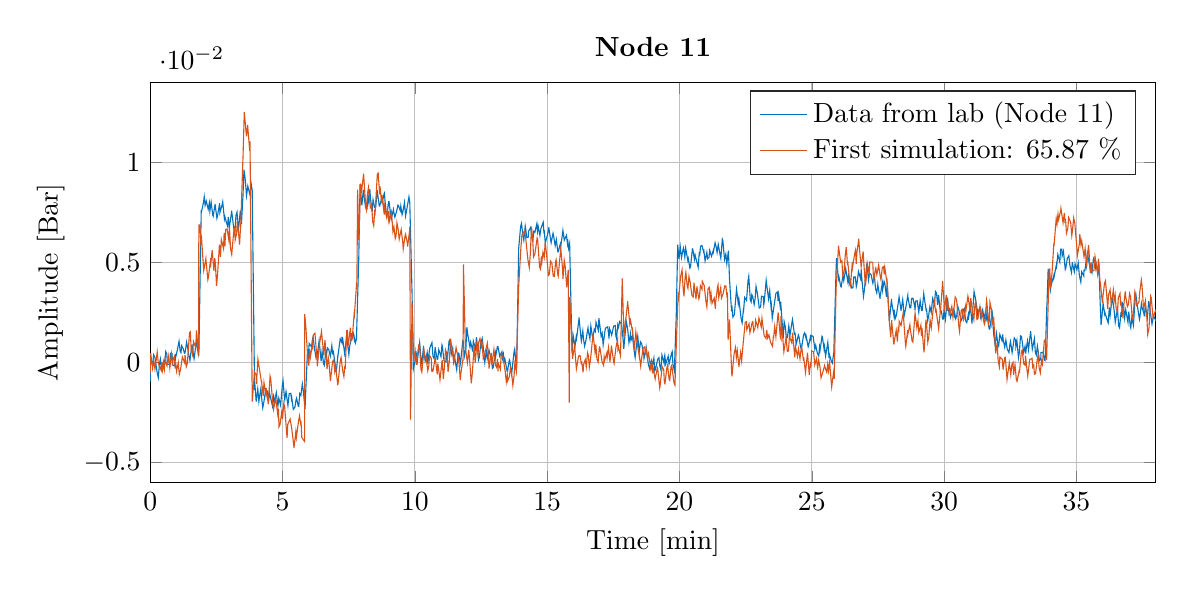
\begin{tikzpicture}

\begin{axis}[%
width=5.028in,
height=2in,
at={(1.011in,0.642in)},
scale only axis,
xmin=0,
xmax=38,
xlabel={Time [min]},
xmajorgrids,
ymin=-0.006,
ymax=0.014,
ylabel={Amplitude [Bar]},
ymajorgrids,
axis background/.style={fill=white},
title style={font=\bfseries},
title={Node 11},
legend style={legend cell align=left,align=left,draw=white!15!black}
]
\addplot [color=mycolor1,solid]
  table[row sep=crcr]{%
0.000833333333333333	-0.00095383988269801\\
0.00916666666666667	0.000151917693059583\\
0.09	-8.47196480935342e-05\\
0.13	0.000384205083089034\\
0.180833333333333	0.000238046725317048\\
0.264166666666667	-0.000527544672531327\\
0.304166666666667	-0.000759832062560556\\
0.350833333333333	-5.2530009775037e-05\\
0.3825	0.000171927468231248\\
0.434166666666667	-0.000395306158357617\\
0.480833333333333	-0.000334406842619622\\
0.519166666666667	0.000117988074292474\\
0.535	-0.000177808602149693\\
0.585833333333333	0.000546893255131881\\
0.626666666666667	0.000421614662755809\\
0.649166666666667	-7.42797653964511e-05\\
0.740833333333333	-0.000104729423265532\\
0.77	0.000461634213097861\\
0.820833333333333	0.000445974389052001\\
0.854166666666667	-0.000138659042036304\\
0.924166666666667	-0.000175198631476498\\
0.964166666666667	0.000420744672534612\\
0.971666666666667	0.000323305767353732\\
1.0325	0.000669561876831926\\
1.08833333333333	0.00106018748777539\\
1.1325	0.00055820312805363\\
1.16166666666667	0.00049295386119258\\
1.18833333333333	0.00083660000000027\\
1.245	0.000691311632451924\\
1.2925	0.000463374193545057\\
1.315	0.00048338396871625\\
1.375	0.00102190791788676\\
1.42	0.000681741739978425\\
1.4675	0.000281546236560404\\
1.49916666666667	0.00010145826001956\\
1.57333333333333	0.00087400957966613\\
1.57916666666667	0.000877489540565463\\
1.6575	0.00018236735092611\\
1.66583333333333	0.000243266666663938\\
1.73333333333333	0.000999288172042562\\
1.755	0.00100102815249098\\
1.81583333333333	0.000417264711623871\\
1.84	0.000611272531764628\\
1.9275	0.00761208387095852\\
1.93666666666667	0.0075459646138761\\
2.015	0.00801923929618911\\
2.04	0.00828632629521028\\
2.07333333333333	0.00785742111436821\\
2.11666666666667	0.00807578866079486\\
2.19	0.00766515327467945\\
2.2325	0.00797747976538976\\
2.25333333333333	0.00757119433039297\\
2.3	0.00802358924730914\\
2.36166666666667	0.00737196656891331\\
2.38	0.00731715718474962\\
2.45166666666667	0.00792963030302407\\
2.4525	0.00789483069403052\\
2.51916666666667	0.00721710830889397\\
2.54	0.00731889716520021\\
2.6225	0.0079609499511179\\
2.63333333333333	0.00750420508308383\\
2.71333333333333	0.00786090107526083\\
2.73916666666667	0.00802793919843273\\
2.80333333333333	0.00716751886607983\\
2.8225	0.00728496754642624\\
2.885	0.0069752510263861\\
2.92166666666667	0.00682735268816476\\
2.94833333333333	0.00726234780058665\\
2.9875	0.00675166353861417\\
3.06583333333333	0.00744156578690183\\
3.075	0.00759381407624393\\
3.15333333333333	0.00673861368524417\\
3.19666666666667	0.0064480369501482\\
3.23916666666667	0.00735456676441618\\
3.27916666666667	0.00752160488758666\\
3.32333333333333	0.00669163421309596\\
3.3475	0.00680908289344306\\
3.405	0.00760860391006307\\
3.4475	0.00693697145649355\\
3.50166666666667	0.00828980625610715\\
3.50333333333333	0.00828545630498215\\
3.5425	0.00963568113391491\\
3.59083333333333	0.00914500664710974\\
3.63833333333333	0.00834461564027511\\
3.6875	0.00881876031280346\\
3.76583333333333	0.00839333509286394\\
3.7675	0.00833939569892625\\
3.81333333333333	0.00894403890517598\\
3.85333333333333	0.00860387272726162\\
3.94166666666667	-0.00118090733138271\\
3.955	-0.0011052181818243\\
4.00416666666667	-0.00195780860215816\\
4.06333333333333	-0.00132358572825805\\
4.10583333333333	-0.00195258866081213\\
4.11916666666667	-0.00181426021506464\\
4.18083333333333	-0.00130444594331602\\
4.205	-0.00171421133921396\\
4.2525	-0.00226839511242499\\
4.29916666666667	-0.00193953880743433\\
4.36166666666667	-0.00135229540566112\\
4.42916666666667	-0.00143581446724991\\
4.46083333333333	-0.0018542797654035\\
4.47833333333333	-0.00186558963831654\\
4.5025	-0.00148540391007113\\
4.61583333333333	-0.00216573626587999\\
4.64	-0.00173596109480623\\
4.65916666666667	-0.00165853196480295\\
4.68583333333333	-0.00203262776147706\\
4.76416666666667	-0.00150454369501457\\
4.81666666666667	-0.00210222697947696\\
4.825	-0.00216921622679248\\
4.85916666666667	-0.00178294056697009\\
4.9275	-0.00213963655913996\\
4.99083333333333	-0.00116698748777819\\
5.01833333333333	-0.000914690322571188\\
5.07416666666667	-0.00178903049853996\\
5.08333333333333	-0.00185862971651996\\
5.13083333333333	-0.00146017419353367\\
5.20333333333333	-0.00214398651025502\\
5.25083333333333	-0.00156109305962954\\
5.31083333333333	-0.00154282326491992\\
5.33916666666667	-0.00183253000978137\\
5.34916666666667	-0.0017768506353931\\
5.40583333333333	-0.00234321427174816\\
5.46666666666667	-0.00223794545453582\\
5.51	-0.0018734195503384\\
5.53	-0.00178381055719254\\
5.59333333333333	-0.00217878611926489\\
5.61333333333333	-0.00219444594330437\\
5.64833333333333	-0.0015576130987156\\
5.6925	-0.00164635210164615\\
5.7475	-0.00107302854349167\\
5.7825	-0.0013975348973673\\
5.85	-0.00232842443793113\\
5.8675	-0.00171421133920258\\
5.93416666666667	0.00034244555229182\\
5.9675	0.000240656695986302\\
6.00583333333333	0.000950568719447681\\
6.095	0.000782660606056168\\
6.13	0.00116197634407772\\
6.15333333333333	0.00127159511240368\\
6.21583333333333	0.000585172825033481\\
6.2175	0.000636502248296755\\
6.26666666666667	0.00022760684262127\\
6.3175	0.000429444574776061\\
6.38166666666667	0.00109237712610058\\
6.395	0.000916639100681543\\
6.45833333333333	6.40486803462625e-05\\
6.49333333333333	0.000558203128052576\\
6.55	-6.12299120248405e-05\\
6.5775	-0.00014300899316308\\
6.63666666666667	0.0005590731182821\\
6.65833333333333	0.000384205083088368\\
6.6975	0.000726111241434096\\
6.74333333333333	0.000659121994131373\\
6.80416666666667	0.000313735874873128\\
6.8625	0.000846169892460613\\
6.88916666666667	0.000466854154429125\\
6.91916666666667	0.000544283284445196\\
7.00583333333333	-0.000256107722388738\\
7.03583333333333	-0.000403136070390497\\
7.09166666666667	0.00038768504397671\\
7.09416666666667	0.000345925513187267\\
7.17833333333333	0.00117763616814134\\
7.24166666666667	0.00099406823069903\\
7.24666666666667	0.00124984535680003\\
7.26833333333333	0.00123766549364607\\
7.34666666666667	0.000441624437922922\\
7.3575	0.000521663538607747\\
7.41916666666667	0.00132205454545589\\
7.44333333333333	0.00108628719452786\\
7.50583333333333	0.00040160488757271\\
7.53083333333333	0.000740031085037202\\
7.61666666666667	0.00143863323559404\\
7.66916666666667	0.00149779257088486\\
7.705	0.00119677595308479\\
7.71083333333333	0.00126028523948921\\
7.7525	0.000982758357777447\\
7.79333333333333	0.00118111612905242\\
7.88166666666667	0.00530051984360685\\
7.92916666666667	0.00893011906158284\\
7.9975	0.0078539411534877\\
8.055	0.00864476226782931\\
8.05666666666667	0.00859169286411832\\
8.13916666666667	0.00772344261978622\\
8.19333333333333	0.00768951300100587\\
8.22833333333333	0.00836723538612039\\
8.255	0.00807752864124045\\
8.29833333333333	0.00866042209188725\\
8.32333333333333	0.00820715718478485\\
8.385	0.00753639472142145\\
8.42	0.00813929794722984\\
8.47916666666667	0.0077538922776427\\
8.52	0.00777303206256197\\
8.57666666666667	0.0086134426197646\\
8.58166666666667	0.00853601348975136\\
8.65583333333333	0.00782349149561415\\
8.67083333333333	0.00782523147606473\\
8.73333333333333	0.00814973782993325\\
8.76416666666667	0.00799487956989256\\
8.84416666666667	0.00846815425222761\\
8.84833333333333	0.00847772414470574\\
8.91916666666667	0.00735804672531518\\
8.94	0.00728148758551303\\
9.00666666666667	0.00803837908113966\\
9.02333333333333	0.0080453390029476\\
9.10666666666667	0.00716838885629731\\
9.19	0.00764862346041473\\
9.195	0.00757902424242904\\
9.24333333333333	0.00727104770282669\\
9.30166666666667	0.00751029501463168\\
9.36083333333333	0.00787047096773966\\
9.38083333333333	0.00784263128054197\\
9.44833333333333	0.00759207409578838\\
9.46916666666667	0.00782697145651529\\
9.51666666666667	0.0073919763441069\\
9.54916666666667	0.00755553450637197\\
9.6075	0.00800009951124142\\
9.64833333333333	0.00733194701857659\\
9.72	0.00784089130009993\\
9.77583333333333	0.0082837163244989\\
9.8075	0.00799922952100476\\
9.895	0.00339872121211049\\
9.94083333333333	-0.000345716715551669\\
10.0208333333333	0.000158007624622813\\
10.0383333333333	0.000559073118245157\\
10.0916666666667	6.14387096704028e-05\\
10.15	0.000716541348984412\\
10.18	0.00100102815248423\\
10.2433333333333	1.09792766494754e-05\\
10.2633333333333	-8.3849657838142e-05\\
10.3266666666667	0.000821810166186793\\
10.3333333333333	0.00067826177908617\\
10.3883333333333	7.62285434888488e-05\\
10.4658333333333	0.000499913782999822\\
10.4916666666667	-7.601974583335e-05\\
10.51	0.000221516911057096\\
10.5666666666667	0.00073916109482472\\
10.6458333333333	0.000992328250225716\\
10.6833333333333	0.000311995894406919\\
10.7283333333333	0.000194547214061952\\
10.7675	0.000760910850451102\\
10.7708333333333	0.000695661583588997\\
10.8441666666667	0.000160617595278773\\
10.8641666666667	0.000175407429105739\\
10.9033333333333	0.000643462170046433\\
10.9866666666667	0.000291116129025715\\
11.0233333333333	0.000871399608993823\\
11.0391666666667	0.000807020332351305\\
11.1016666666667	8.40584555192314e-05\\
11.1758333333333	2.92490713548477e-05\\
11.2083333333333	0.000408564809376372\\
11.2325	0.000251096578682608\\
11.2908333333333	0.00106105747800886\\
11.3158333333333	0.00112108680352496\\
11.3741666666667	0.000403344868027539\\
11.4308333333333	0.00072176129030202\\
11.4658333333333	4.31689149451575e-05\\
11.4991666666667	0.000297206060571431\\
11.5408333333333	-6.12299120546778e-05\\
11.5816666666667	-0.000365726490724638\\
11.6333333333333	0.000474684066466613\\
11.6641666666667	0.000451194330403887\\
11.7166666666667	-6.81898338427411e-05\\
11.735	9.18883675354032e-05\\
11.8108333333333	0.00108802717495851\\
11.8291666666667	0.00105061759529979\\
11.8716666666667	0.00031721583576716\\
11.9275	0.000671301857292445\\
11.965	0.00176400957966796\\
11.9966666666667	0.00141862346037275\\
12.0816666666667	0.000767870772216434\\
12.1083333333333	0.00101581798627709\\
12.1691666666667	0.000662601955031095\\
12.18	0.000546893255145203\\
12.2091666666667	0.001072367350929\\
12.29	0.000690441642225925\\
12.3283333333333	0.00126376520042018\\
12.355	0.000929688954076413\\
12.4033333333333	0.00012059804496406\\
12.4366666666667	0.000258926490684569\\
12.4891666666667	0.000950568719426365\\
12.5441666666667	0.00120808582597368\\
12.6091666666667	0.000486863929612058\\
12.6433333333333	4.88934505260552e-06\\
12.6966666666667	0.000550373216017919\\
12.7016666666667	0.000574732942314471\\
12.7366666666667	0.000198897165199746\\
12.8008333333333	0.000618232453555884\\
12.8716666666667	0.000221516911017294\\
12.8775	0.000354625415417364\\
12.9325	-0.000291777321623915\\
12.96	-0.000255237732179087\\
13.04	0.000447714369482849\\
13.05	0.000280676246319472\\
13.1183333333333	0.000800930400774336\\
13.1391666666667	0.000797450439870367\\
13.2066666666667	0.000308515933525683\\
13.2908333333333	0.000537323362652886\\
13.3083333333333	0.000194547214053431\\
13.345	0.000421614662730052\\
13.3741666666667	6.31786900953946e-05\\
13.4016666666667	0.000178887390009708\\
13.485	-0.000433585728254082\\
13.4991666666667	-0.000446635581630467\\
13.57	0.000136257869004952\\
13.585	9.97182795516027e-05\\
13.6533333333333	-0.000565824242423185\\
13.6675	-0.000444025610948945\\
13.7466666666667	0.000523403519034155\\
13.7725	0.000668691886608064\\
13.835	-0.000247407820120282\\
13.8458333333333	-0.000255237732159186\\
13.9225	0.00569549540567496\\
13.9966666666667	0.00680473294231948\\
14.03	0.00695785122186696\\
14.0816666666667	0.00635842795697389\\
14.1166666666667	0.00611309071358054\\
14.1708333333333	0.00682039276639448\\
14.185	0.00670207409580431\\
14.2325	0.00624532922776955\\
14.2858333333333	0.00626794897361552\\
14.3	0.00657331554252782\\
14.3758333333333	0.00675688347996586\\
14.4366666666667	0.00610178084068028\\
14.4558333333333	0.00605828132945024\\
14.4941666666667	0.00656809560117327\\
14.5358333333333	0.00651067624629323\\
14.6091666666667	0.00694132140764059\\
14.6341666666667	0.00655591573804207\\
14.6591666666667	0.00680995288368255\\
14.725	0.006354078005856\\
14.7625	0.00669163421312366\\
14.85	0.00701266060604558\\
14.8783333333333	0.00646021681327799\\
14.8883333333333	0.00660289521014482\\
14.9275	0.0059791122189751\\
15.0175	0.00641062737046813\\
15.0608333333333	0.00673687370476447\\
15.0616666666667	0.00673774369498975\\
15.1483333333333	0.005989552101687\\
15.2216666666667	0.00646282678397941\\
15.2383333333333	0.00636625786900996\\
15.3025	0.00583817380251336\\
15.3458333333333	0.00614963030301116\\
15.4041666666667	0.00552758729227779\\
15.4175	0.00552845728251444\\
15.4891666666667	0.00589820312807493\\
15.505	0.00573464496579848\\
15.5841666666667	0.0064810965786791\\
15.595	0.00660289521016755\\
15.6458333333333	0.00611657067450441\\
15.7283333333333	0.00635755796669746\\
15.7616666666667	0.00600173196481255\\
15.7716666666667	0.00617051006842079\\
15.8125	0.00569897536653347\\
15.8491666666667	0.00594779257080522\\
15.9366666666667	0.000632152297163235\\
15.945	0.000493823851428515\\
15.9808333333333	0.00135337419355328\\
16.0508333333333	0.000810500293255273\\
16.0975	0.00129508484842522\\
16.1116666666667	0.00120808582596513\\
16.1991666666667	0.00215724516131677\\
16.2025	0.00225120410559046\\
16.2858333333333	0.00110977693057071\\
16.2908333333333	0.00106801739978554\\
16.3466666666667	0.00157174173992305\\
16.3741666666667	0.0011480565004604\\
16.415	0.000813110263908401\\
16.4616666666667	0.00108802717495568\\
16.5425	0.00173007996082791\\
16.5566666666667	0.00156913176923584\\
16.615	0.0011872060605356\\
16.65	0.00181881896380109\\
16.7083333333333	0.00128638494624059\\
16.7325	0.00126115522973583\\
16.7783333333333	0.00166048074290193\\
16.8175	0.00155173196476999\\
16.8441666666667	0.00201456676442152\\
16.9325	0.00161263128053979\\
16.9541666666667	0.00221466451606606\\
16.9908333333333	0.00185274858254164\\
17.0375	0.00132118455520075\\
17.0766666666667	0.00146647292276048\\
17.115	0.00089053939390174\\
17.1625	0.00136294408598592\\
17.1991666666667	0.00171355014659871\\
17.2875	0.00178227937444153\\
17.3366666666667	0.00123418553279184\\
17.3383333333333	0.00123853548391256\\
17.3591666666667	0.00168919042034762\\
17.4366666666667	0.00137338396871203\\
17.5116666666667	0.00181794897357013\\
17.5716666666667	0.00184317869013176\\
17.595	0.00132205454543172\\
17.6191666666667	0.00120634584552595\\
17.6683333333333	0.0018858082111706\\
17.6975	0.00175791964812225\\
17.7358333333333	0.0020415364614394\\
17.8116666666667	0.001922347800587\\
17.8608333333333	0.00126202521994973\\
17.8941666666667	0.00067826177908617\\
17.95	0.0015099724339962\\
17.9933333333333	0.00201630674484934\\
18.0383333333333	0.00170833020525268\\
18.09	0.000993198240445331\\
18.1491666666667	0.00143776324532044\\
18.1675	0.00110716695990054\\
18.22	0.00132988445751042\\
18.2966666666667	0.000485123949187066\\
18.3241666666667	0.000254576539595097\\
18.3766666666667	0.000867919648061433\\
18.4216666666667	0.00131248465294223\\
18.4716666666667	0.000639112218982552\\
18.4816666666667	0.000579952883686063\\
18.5283333333333	0.0010288678396535\\
18.5708333333333	0.000937518866055642\\
18.6508333333333	0.000383335092846021\\
18.6591666666667	0.000198027174940357\\
18.7383333333333	0.000712191397843787\\
18.7408333333333	0.00074438103617358\\
18.8233333333333	-0.000109079374419674\\
18.8725	-0.000315267057646867\\
18.9133333333333	1.96791789108253e-05\\
18.9358333333333	0.000111898142705541\\
18.985	-0.000127349169167651\\
19.0316666666667	0.000215426979417593\\
19.0658333333333	-0.000415315933525978\\
19.0966666666667	-0.000317877028351149\\
19.175	0.000164967546419398\\
19.2233333333333	0.000245006647139723\\
19.2558333333333	-0.00017606862169825\\
19.2966666666667	-0.000363986510325237\\
19.3366666666667	0.000378115151437486\\
19.4208333333333	-5.25300097933279e-05\\
19.4383333333333	0.000325915738011467\\
19.4441666666667	0.000363325317675883\\
19.4783333333333	-8.12396871878729e-05\\
19.5725	0.000313735874857501\\
19.6041666666667	-7.86297165404626e-05\\
19.6133333333333	-3.42602150623927e-05\\
19.6975	0.000445104398852481\\
19.7241666666667	0.000539933333323056\\
19.7525	-9.42895405671162e-05\\
19.8058333333333	-0.000406616031250417\\
19.8766666666667	0.00231906334311138\\
19.9325	0.00588602326492951\\
19.9791666666667	0.00517263128053291\\
20.0291666666667	0.00578336441837454\\
20.075	0.00524136050829616\\
20.1325	0.00564242600194123\\
20.1525	0.00572768504396212\\
20.2008333333333	0.00527268015637222\\
20.2316666666667	0.00571985513194026\\
20.3141666666667	0.00510303206247617\\
20.3316666666667	0.00519699100676124\\
20.3908333333333	0.00471762639293163\\
20.4158333333333	0.00476982580642019\\
20.4883333333333	0.00568418553273778\\
20.4991666666667	0.00568244555228151\\
20.565	0.0051569714564437\\
20.59	0.00537446901266211\\
20.6625	0.00498645337245879\\
20.705	0.00476025591393639\\
20.7508333333333	0.00554063714561726\\
20.7641666666667	0.00535010928639967\\
20.795	0.00581990400780233\\
20.8491666666667	0.00584600371451532\\
20.9208333333333	0.00548669775168381\\
20.9266666666667	0.00552410733134825\\
20.9666666666667	0.00507780234596569\\
21.0333333333333	0.00550496754640908\\
21.0625	0.00518742111440251\\
21.1141666666667	0.0052578903225822\\
21.1408333333333	0.00560936637342596\\
21.2091666666667	0.00530834975562589\\
21.2758333333333	0.00559979648090805\\
21.2825	0.00554585708697464\\
21.345	0.00598520215052081\\
21.385	0.00577379452586801\\
21.4208333333333	0.00550235757571618\\
21.4633333333333	0.00590255307917009\\
21.5358333333333	0.00537620899312974\\
21.5616666666667	0.00520917087002321\\
21.6183333333333	0.00616790009777904\\
21.6366666666667	0.00611657067448737\\
21.7016666666667	0.00514827155422498\\
21.7508333333333	0.00541535855323905\\
21.7875	0.00494382385140288\\
21.8491666666667	0.00559109657864956\\
21.89	0.00415909266857856\\
21.9625	0.00266357947209034\\
21.9841666666667	0.00274535855321578\\
22.0166666666667	0.00227121388072651\\
22.0725	0.00239040254152204\\
22.1525	0.00362230869978367\\
22.1558333333333	0.00366667820125602\\
22.22	0.00293762639292941\\
22.2441666666667	0.00317078377319152\\
22.3283333333333	0.00219204477029397\\
22.3675	0.00197976715549547\\
22.4133333333333	0.00263486979477537\\
22.4233333333333	0.0026052901271385\\
22.4608333333333	0.00325082287390618\\
22.5333333333333	0.00309944457472403\\
22.5891666666667	0.00408862346039887\\
22.6175	0.00430612101664568\\
22.6758333333333	0.00313076422285694\\
22.7083333333333	0.00302810537628492\\
22.7333333333333	0.00339176129028265\\
22.7683333333333	0.00329519237533307\\
22.8208333333333	0.002899346823034\\
22.8566666666667	0.00317774369498242\\
22.8916666666667	0.00380239667641721\\
22.9416666666667	0.00346397047890723\\
23.0141666666667	0.0027253487780968\\
23.065	0.00277406823070128\\
23.0966666666667	0.0033143321603632\\
23.1625	0.00329780234601462\\
23.185	0.00289151691100645\\
23.2033333333333	0.00304289521011472\\
23.2758333333333	0.00410602326493295\\
23.2941666666667	0.00390244555230201\\
23.3658333333333	0.00318122365590059\\
23.4083333333333	0.00358924907134228\\
23.4566666666667	0.00281147781037139\\
23.4691666666667	0.00289673685239225\\
23.505	0.0022129245356837\\
23.5591666666667	0.00270359902247042\\
23.6416666666667	0.0034578805473473\\
23.7033333333333	0.003525739784908\\
23.7241666666667	0.00307160488755476\\
23.7508333333333	0.00337871143694318\\
23.8025	0.00281669775172877\\
23.8233333333333	0.00303680527858891\\
23.9025	0.00156652179854863\\
23.9258333333333	0.00137338396863246\\
23.955	0.00204153646132002\\
23.9925	0.00183708875855476\\
24.0408333333333	0.00119155601171886\\
24.0808333333333	0.00128203499511417\\
24.13	0.00182316891497866\\
24.1733333333333	0.00135250420333935\\
24.2541666666667	0.00203892649072376\\
24.27	0.00214941524923806\\
24.3416666666667	0.00142384340170457\\
24.3683333333333	0.00145081309867126\\
24.4091666666667	0.00091837908109374\\
24.4375	0.00106105747801169\\
24.4916666666667	0.00137164398830694\\
24.5166666666667	0.00128377497560453\\
24.5775	0.000733071163239202\\
24.615	0.000750470967756239\\
24.6891666666667	0.00137773391983279\\
24.7283333333333	0.00148126275659027\\
24.7775	0.00123070557186228\\
24.7858333333333	0.00131248465300476\\
24.8633333333333	0.000783530596288579\\
24.8683333333333	0.000802670381244791\\
24.9475	0.00127942502449518\\
24.9691666666667	0.00114979648095645\\
24.9816666666667	0.00135337419351916\\
25.0508333333333	0.0013037847507292\\
25.1141666666667	0.000667821896354365\\
25.1475	0.000864439687188717\\
25.2083333333333	0.000462504203301295\\
25.2616666666667	0.000332875659830784\\
25.2925	0.000778310654965281\\
25.3108333333333	0.000614752492680309\\
25.385	0.00130900469207521\\
25.4008333333333	0.00127594506351447\\
25.4633333333333	0.000670431867035887\\
25.48	0.000805280351914961\\
25.5208333333333	0.000327655718456332\\
25.605	0.00100711808407827\\
25.6533333333333	0.000210207038145477\\
25.665	0.000400734897380101\\
25.7416666666667	5.01288367047714e-05\\
25.7766666666667	-3.25202346231901e-05\\
25.8283333333333	0.000482513978499854\\
25.83	0.000435534506357305\\
25.9175	0.00467586686218627\\
25.935	0.00521352082110985\\
26.005	0.00417475249266208\\
26.025	0.00427480136854119\\
26.0883333333333	0.00381892649074875\\
26.1091666666667	0.00377977693063375\\
26.1758333333333	0.00436006041047679\\
26.2075	0.00409558338212723\\
26.2675	0.00456102815246598\\
26.2808333333333	0.00469500664707997\\
26.3558333333333	0.00406513372433895\\
26.3833333333333	0.00431743088950046\\
26.4108333333333	0.00390505552294376\\
26.45	0.00411298318667835\\
26.5033333333333	0.00372322756593921\\
26.5533333333333	0.00373366744868808\\
26.5866666666667	0.00427741133919429\\
26.6433333333333	0.00427480136854119\\
26.6808333333333	0.00379543675464336\\
26.7066666666667	0.00393985513196643\\
26.7633333333333	0.00454536832849617\\
26.8466666666667	0.0041756224828419\\
26.8683333333333	0.00465324711627207\\
26.8825	0.00430873098727039\\
26.9516666666667	0.00330563225804217\\
26.9866666666667	0.00362230869990302\\
27.0558333333333	0.00460365767349916\\
27.0833333333333	0.00498297341154061\\
27.1408333333333	0.0041312529814434\\
27.1433333333333	0.00415387272728371\\
27.18	0.0044574993157028\\
27.2375	0.00440442991197759\\
27.3041666666667	0.0039824846529655\\
27.3666666666667	0.00433744066468197\\
27.4058333333333	0.00370060782009321\\
27.4541666666667	0.00347702033228078\\
27.4925	0.00388678572824122\\
27.4933333333333	0.00387373587487336\\
27.5791666666667	0.00318818357771991\\
27.5816666666667	0.00328997243402118\\
27.6633333333333	0.00396508484853375\\
27.6741666666667	0.00363622854353599\\
27.7316666666667	0.00405904379273356\\
27.7575	0.00397378475073543\\
27.8208333333333	0.00328040254159423\\
27.8475	0.00394507507336361\\
27.9283333333333	0.00209634584549012\\
27.9316666666667	0.00209895581617164\\
28.0116666666667	0.00317687370477987\\
28.0191666666667	0.00299591573801766\\
28.0991666666667	0.00237039276634055\\
28.1133333333333	0.00264356969694293\\
28.1475	0.00217986490713432\\
28.1958333333333	0.00236604281519706\\
28.28	0.00309596461389677\\
28.2975	0.00327953255135188\\
28.3691666666667	0.00261746999025267\\
28.37	0.00258963030305498\\
28.435	0.00314642404696319\\
28.46	0.00282365767356513\\
28.4858333333333	0.00232254330402387\\
28.5441666666667	0.00268967917884314\\
28.6275	0.00335870166176169\\
28.6316666666667	0.00327431260996039\\
28.7041666666667	0.00273926862170701\\
28.7391666666667	0.00273578866080587\\
28.7708333333333	0.00319949345063156\\
28.8233333333333	0.00321515327472643\\
28.895	0.00274535855324989\\
28.9008333333333	0.00262355992177279\\
28.9216666666667	0.00307073489734083\\
28.9833333333333	0.00308378475072008\\
29.0425	0.0025165511241369\\
29.0941666666667	0.00309248465301271\\
29.1458333333333	0.00260181016616348\\
29.17	0.00259572023459786\\
29.2291666666667	0.00343961075270163\\
29.245	0.0032777925708786\\
29.3283333333333	0.00254613079175106\\
29.3325	0.00269750909088207\\
29.3791666666667	0.00208764594326571\\
29.4208333333333	0.00239823245353254\\
29.4616666666667	0.0027905980449589\\
29.5116666666667	0.00250350127074062\\
29.5675	0.00320384340172955\\
29.6325	0.00290021681329908\\
29.6741666666667	0.00355096950140141\\
29.7133333333333	0.00347702033230352\\
29.7541666666667	0.00288368699898459\\
29.7883333333333	0.00337784144668948\\
29.855	0.00255483069400389\\
29.8958333333333	0.00257136050826151\\
29.9425	0.00217638494622752\\
29.9733333333333	0.00217290498534911\\
29.995	0.00263312981431343\\
30.0491666666667	0.00216072512222926\\
30.1166666666667	0.003112494428126\\
30.1325	0.00317600371450913\\
30.1816666666667	0.00246435171067677\\
30.21	0.00261833998048933\\
30.24	0.00225207409581576\\
30.3458333333333	0.00265748954055314\\
30.3816666666667	0.00237474271747265\\
30.3958333333333	0.00250524125118548\\
30.4375	0.00218943479958403\\
30.4758333333333	0.00232602326486248\\
30.515	0.00280973782982988\\
30.56	0.00260790009767223\\
30.6358333333333	0.00207807605082738\\
30.6791666666667	0.00220770459428654\\
30.7266666666667	0.00263312981425093\\
30.7625	0.0027018590420369\\
30.8141666666667	0.0020754660802027\\
30.8558333333333	0.00199455698929119\\
30.9066666666667	0.00235212297161527\\
30.9133333333333	0.00213462541542531\\
30.9941666666667	0.00284105747795141\\
30.9958333333333	0.00279494799603416\\
31.0525	0.0019440975561395\\
31.0833333333333	0.00263921974577105\\
31.1308333333333	0.00355009951113064\\
31.1758333333333	0.00324647292273997\\
31.2583333333333	0.00257484046917969\\
31.2683333333333	0.00239562248290784\\
31.3458333333333	0.00271838885629452\\
31.3491666666667	0.00274709853371183\\
31.3741666666667	0.00226599393936913\\
31.4558333333333	0.00264095972628983\\
31.5125	0.00217725493646984\\
31.5541666666667	0.00249045141742391\\
31.5825	0.00205458631474476\\
31.6125	0.00246000175946509\\
31.695	0.00171616011738823\\
31.7225	0.0016717906159045\\
31.7841666666667	0.00224859413492032\\
31.8083333333333	0.00264617966766426\\
31.8716666666667	0.00142384340178414\\
31.9308333333333	0.000842689931579377\\
31.9758333333333	0.00145429305953829\\
32.0308333333333	0.000947088758545128\\
32.0608333333333	0.000829640078194444\\
32.105	0.00140209364619184\\
32.1875	0.00108976715562795\\
32.2141666666667	0.00140644359746037\\
32.2275	0.00117763616826214\\
32.2891666666667	0.000768740762481485\\
32.3333333333333	0.00112108680359033\\
32.3841666666667	0.000672171847594466\\
32.45	0.000492953861106621\\
32.4841666666667	0.000902719257061368\\
32.5075	0.0010514875855677\\
32.5691666666667	0.000499043792768855\\
32.5725	0.000527753470197512\\
32.6508333333333	0.00122722561091568\\
32.6983333333333	0.0011158668621363\\
32.71	0.000797450439841946\\
32.75	0.00109498709674088\\
32.8091666666667	0.000236306744881204\\
32.84	0.00048338396869102\\
32.8866666666667	0.001331624437961\\
32.9233333333333	0.00130030478983945\\
33.0058333333333	0.000499043792700632\\
33.0558333333333	0.000796580449656442\\
33.0858333333333	0.00044945435005847\\
33.0975	0.000645202150616392\\
33.1508333333333	0.0010767173020611\\
33.1883333333333	0.000642592179877999\\
33.2691666666667	0.00156913176918469\\
33.2725	0.00150823245342627\\
33.3316666666667	0.000665211925655773\\
33.4116666666667	0.00119242600196121\\
33.4466666666667	0.000496433822144177\\
33.4816666666667	0.000374635190650036\\
33.525	0.000818330205351048\\
33.535	0.000725241251262831\\
33.6025	9.10183773215056e-05\\
33.6516666666667	0.000162357575862915\\
33.6583333333333	0.00049121388086068\\
33.7341666666667	0.000511223655934173\\
33.7908333333333	0.000124078005723088\\
33.8158333333333	9.62383185936222e-05\\
33.8816666666667	0.00287933704792639\\
33.8858333333333	0.00286715718481792\\
33.9308333333333	0.00467760684275054\\
34.0141666666667	0.00361708875857975\\
34.06	0.0040216342129327\\
34.0658333333333	0.00396334486787855\\
34.145	0.00435484046933543\\
34.1516666666667	0.00425827155436881\\
34.2358333333333	0.00484899491695504\\
34.24	0.00466890694042948\\
34.2966666666667	0.00539534877812575\\
34.3716666666667	0.00502821290322689\\
34.4	0.00566330576741056\\
34.4458333333333	0.00566939569902733\\
34.4608333333333	0.00532574956021681\\
34.5083333333333	0.00555977693069853\\
34.5775	0.00465672707724143\\
34.6	0.00473502619744867\\
34.6541666666667	0.00520656089930188\\
34.7141666666667	0.00533705943284421\\
34.75	0.00486639472129016\\
34.8125	0.00450795874891699\\
34.8458333333333	0.00501255307929685\\
34.8483333333333	0.00496296363648416\\
34.9191666666667	0.00454101837730722\\
34.9475	0.00493686392957787\\
35.0175	0.00464367722383377\\
35.0675	0.00498036344086475\\
35.1108333333333	0.00434266060607916\\
35.165	0.00401902424248993\\
35.1983333333333	0.00453666842616376\\
35.2766666666667	0.00432874076234957\\
35.2858333333333	0.00461583753652239\\
35.3216666666667	0.00461322756576127\\
35.36	0.00501690303016747\\
35.3783333333333	0.00484725493641353\\
35.4108333333333	0.00546842795696992\\
35.4658333333333	0.00508302228737992\\
35.5191666666667	0.00466455698925192\\
35.585	0.00447489912007204\\
35.6366666666667	0.0051421816225741\\
35.6558333333333	0.00522222072330014\\
35.7208333333333	0.00475416598233669\\
35.7291666666667	0.00504213274676321\\
35.8075	0.00448968895405533\\
35.8475	0.00500994310855848\\
35.8991666666667	0.00287411710651786\\
35.9	0.00289151691101214\\
35.93	0.00188058826979048\\
36.0083333333333	0.00294197634415813\\
36.065	0.00243912199419474\\
36.0741666666667	0.00249654134908614\\
36.1583333333333	0.00213636539589859\\
36.2	0.00197976715540452\\
36.2425	0.0027549284457962\\
36.2725	0.00236169286410476\\
36.3075	0.00277232825016543\\
36.3583333333333	0.00322472316716474\\
36.4241666666667	0.00259833020524528\\
36.4658333333333	0.00201804672529424\\
36.5483333333333	0.00267314936447183\\
36.5975	0.00182316891492182\\
36.6283333333333	0.00173616989248448\\
36.6866666666667	0.0025235110458596\\
36.6916666666667	0.00228513372425712\\
36.7458333333333	0.0029532862170584\\
36.775	0.00288629696978551\\
36.8216666666667	0.00221292453568939\\
36.8625	0.00264008973610433\\
36.9475	0.00201195679377977\\
36.9766666666667	0.00254265083096361\\
37.0358333333333	0.00181185904203293\\
37.0516666666667	0.0017335599217802\\
37.0916666666667	0.00221031456495102\\
37.1541666666667	0.00185448856310022\\
37.2125	0.00313163421317886\\
37.2441666666667	0.00342482091879792\\
37.2983333333333	0.00284714740964209\\
37.3	0.00284888739010403\\
37.3808333333333	0.00215898514171048\\
37.3966666666667	0.00226860391006203\\
37.4541666666667	0.00294458631480557\\
37.475	0.00276797829912429\\
37.5625	0.0023790926686218\\
37.5641666666667	0.00230949345063328\\
37.6025	0.00285323734119064\\
37.6825	0.00225555405666572\\
37.7266666666667	0.00304637517106701\\
37.7375	0.003040285239473\\
37.825	0.00221553450632545\\
37.855	0.00192756774194439\\
37.9125	0.00233124320636197\\
38	0.0020885159335933\\
};
\addlegendentry{Data from lab (Node 11)};

\addplot [color=mycolor2,solid]
  table[row sep=crcr]{%
0.000833333333333333	-0.000189777655498596\\
0.00166666666666667	-0.000511418870457609\\
0.0175	0.000470724622740798\\
0.0891666666666667	-0.000292493524285871\\
0.135	9.97011341877142e-05\\
0.178333333333333	-0.000334773420069599\\
0.264166666666667	0.000527247268031176\\
0.305833333333333	-4.6131075658742e-05\\
0.410833333333333	-0.000383300554228232\\
0.4275	2.81514125811318e-05\\
0.4625	-0.000362139845849916\\
0.493333333333333	2.52129284550975e-05\\
0.533333333333333	-0.00033903895260059\\
0.558333333333333	0.000154778229055289\\
0.634166666666667	-0.000173671285907817\\
0.695833333333333	0.000329937605307738\\
0.701666666666667	0.000236934882124811\\
0.74	-0.000269196459369452\\
0.8025	0.000408291746283\\
0.8325	-2.13831981043288e-05\\
0.908333333333333	0.000304170338005623\\
0.945	-0.000303218530930085\\
0.965	-2.94712930654603e-05\\
0.995833333333333	-0.000437966586703698\\
1.05916666666667	-9.38610691790455e-06\\
1.0975	-0.000593963522543755\\
1.14583333333333	-0.000341578012703449\\
1.215	0.000277863705801505\\
1.30333333333333	-2.27805047866539e-05\\
1.315	0.000341590414243\\
1.31583333333333	0.000382481133207476\\
1.36416666666667	-0.000200729234087465\\
1.4025	-4.03612224515419e-05\\
1.485	0.00149710040499545\\
1.51333333333333	0.0015336369284793\\
1.5475	0.000645550512613331\\
1.60166666666667	0.00036936686936749\\
1.63416666666667	0.00104610788782411\\
1.71833333333333	0.000750609396652643\\
1.74833333333333	0.00160642897321785\\
1.83166666666667	0.000330976902555215\\
1.83583333333333	0.00687318146761357\\
1.8775	0.00687315934138102\\
1.91	0.00600523796262491\\
1.93916666666667	0.00620787295107609\\
2.0125	0.00475763774877514\\
2.02166666666667	0.00460513277009943\\
2.10166666666667	0.00518633788085125\\
2.1025	0.00516436775604337\\
2.1775	0.00414044527643303\\
2.19833333333333	0.00426249556112373\\
2.2725	0.00505908614760922\\
2.28833333333333	0.00492168086687631\\
2.34083333333333	0.00561136664070409\\
2.40666666666667	0.00458178077432767\\
2.43916666666667	0.00521796579014857\\
2.46083333333333	0.00495760935447638\\
2.50583333333333	0.00383151619166246\\
2.54416666666667	0.00439447755777642\\
2.61416666666667	0.00588856118752546\\
2.65583333333333	0.00528430719238657\\
2.68666666666667	0.00615374667401178\\
2.76916666666667	0.00569520174005732\\
2.7925	0.00647277361758451\\
2.82166666666667	0.00580741136471557\\
2.85	0.0066432401211457\\
2.90416666666667	0.0066762773791478\\
2.96916666666667	0.00613533210553087\\
2.995	0.00676082135379759\\
3.03333333333333	0.00569757291007997\\
3.07916666666667	0.00540825048248973\\
3.1525	0.00650120957312658\\
3.19	0.00680667548095756\\
3.20916666666667	0.00613212912654184\\
3.2625	0.00642893294726768\\
3.29333333333333	0.00710564083040903\\
3.37666666666667	0.00589401174710646\\
3.415	0.00685753103527079\\
3.41833333333333	0.00680931629165512\\
3.50333333333333	0.010220220165654\\
3.50416666666667	0.0101799575868493\\
3.55333333333333	0.0125227536013572\\
3.63666666666667	0.011305670062478\\
3.67833333333333	0.0118231059955056\\
3.67916666666667	0.0118807172773949\\
3.76	0.0105782946971991\\
3.77083333333333	0.0110616060824888\\
3.85333333333333	-0.00187200089860226\\
3.85666666666667	-0.00195500725995286\\
3.94	-0.00048113230538272\\
3.99333333333333	-0.000579002958502081\\
4.0225	-0.00107562449901524\\
4.03	-0.000700442719375\\
4.06916666666667	0.000164956250876308\\
4.11833333333333	-0.000266269220939799\\
4.20166666666667	-0.000971473597117902\\
4.20416666666667	-0.00089168256085883\\
4.2675	-0.00168189525048202\\
4.29916666666667	-0.00101158590081738\\
4.3675	-0.001567752054271\\
4.37916666666667	-0.00127024016170975\\
4.4625	-0.00208505448802539\\
4.46833333333333	-0.00193705569226268\\
4.52833333333333	-0.000688327203188526\\
4.55416666666667	-0.000827000140859115\\
4.63	-0.00203606129213716\\
4.66083333333333	-0.00234247985478777\\
4.72916666666667	-0.00184375137348148\\
4.73333333333333	-0.00170926741408358\\
4.81666666666667	-0.00258340829072287\\
4.84416666666667	-0.00230376963798622\\
4.86416666666667	-0.00321518286833851\\
4.90583333333333	-0.0030992694796077\\
4.97166666666667	-0.00243997590319427\\
4.99833333333333	-0.00281202585179778\\
5.0475	-0.00204527332318741\\
5.08083333333333	-0.00224365891266729\\
5.16666666666667	-0.00372560516128239\\
5.17083333333333	-0.00376576150605492\\
5.19666666666667	-0.00309167733722427\\
5.285	-0.00283097479409067\\
5.3425	-0.00325603059401209\\
5.43	-0.00421713220654435\\
5.43166666666667	-0.00428069067035348\\
5.50166666666667	-0.00345930432192583\\
5.5225	-0.00374978987399836\\
5.6025	-0.00294911254663742\\
5.64083333333333	-0.00266810815766807\\
5.6925	-0.00313509812408581\\
5.6975	-0.00293236747268447\\
5.7275	-0.00374411490416514\\
5.8325	-0.00394986390798815\\
5.83583333333333	0.00242138664866339\\
5.87666666666667	0.00188159930023844\\
5.94916666666667	0.000271731584583215\\
5.99166666666667	-0.000157562850584896\\
6.02333333333333	0.000662821186565535\\
6.05166666666667	0.000268836145581935\\
6.12916666666667	0.000899393625178726\\
6.14083333333333	0.000815942094841302\\
6.15666666666667	0.00135693861814035\\
6.22416666666667	0.00146602657037975\\
6.305	0.000103432139637914\\
6.31583333333333	-0.000190704492260464\\
6.3925	0.000925719113747624\\
6.39333333333333	0.000889176897798733\\
6.47166666666667	0.00154757320350265\\
6.48083333333333	0.00141472609342412\\
6.56166666666667	0.000341554278524756\\
6.6025	0.00112901613475286\\
6.6525	0.000249270981959076\\
6.68166666666667	-0.000323539151701061\\
6.72583333333333	0.000268953425222781\\
6.74666666666667	0.000107281286311398\\
6.80916666666667	-0.00092265491915681\\
6.835	-0.000624316624327954\\
6.89	5.52196845022376e-05\\
6.93416666666667	0.000122044644934294\\
6.9725	-0.000456191248941403\\
7.00666666666667	-0.000225935593060161\\
7.085	-0.00109344774875706\\
7.095	-0.00107874797668832\\
7.18	6.45194062169047e-05\\
7.2125	0.000247884497452856\\
7.2675	-0.000363061358069072\\
7.3175	-0.000699073551025866\\
7.355	-0.000155169759797584\\
7.3675	-0.000314630663561441\\
7.42666666666667	0.00159220768861648\\
7.45	0.00159937605333\\
7.47416666666667	0.000805686865015218\\
7.565	0.00174247855371942\\
7.58583333333333	0.00108208206113126\\
7.62916666666667	0.00114248207488362\\
7.70583333333333	0.00242898431733215\\
7.715	0.00237744526458126\\
7.79333333333333	0.00385829935637165\\
7.80916666666667	0.00379521754742933\\
7.83583333333333	0.00864091285414981\\
7.88166666666667	0.00610758481015134\\
7.95166666666667	0.0089399052302529\\
7.9775	0.00846114338988882\\
8.05416666666667	0.00933386735735067\\
8.0625	0.00943530969169472\\
8.14416666666667	0.00778193506649362\\
8.16916666666667	0.00763012143002613\\
8.20333333333333	0.00836850764033945\\
8.245	0.00874426463020836\\
8.31916666666667	0.00774447649488609\\
8.36833333333333	0.00785643684192924\\
8.40666666666667	0.00704827174570564\\
8.445	0.00683920408108405\\
8.48083333333333	0.00754434139916971\\
8.4975	0.00747932980200723\\
8.58166666666667	0.0094248672563146\\
8.61333333333334	0.00947109445253628\\
8.66916666666667	0.00841154041408233\\
8.6825	0.0088068419058488\\
8.74166666666667	0.00798471751052978\\
8.7575	0.00838190949126508\\
8.84166666666667	0.00739312727198824\\
8.85	0.00784695113244695\\
8.93083333333333	0.00729594729423585\\
8.95666666666667	0.00767376424163259\\
8.99916666666667	0.00722164042123137\\
9.01916666666667	0.00756105110176951\\
9.03166666666667	0.00703139015533201\\
9.115	0.00751256959128187\\
9.17166666666667	0.00654202950202526\\
9.21	0.00677037413118325\\
9.25833333333333	0.0061945176807255\\
9.29	0.00634234025540843\\
9.32333333333333	0.00698406148433769\\
9.3725	0.00662567132150834\\
9.4075	0.00616813628288588\\
9.48416666666667	0.0066504871123912\\
9.54416666666667	0.00598471970988408\\
9.56083333333333	0.00569060993439739\\
9.6325	0.00635794031361587\\
9.6475	0.00641540043309501\\
9.72	0.00594188216572424\\
9.72583333333333	0.00580075519489449\\
9.8075	0.00667484921840903\\
9.80916666666667	0.00679357905448272\\
9.83583333333333	-0.00285942652632236\\
9.895	0.0030112449597537\\
9.955	7.56147460217382e-05\\
10.0116666666667	0.000584224655955258\\
10.0575	-0.000114885382827403\\
10.0766666666667	0.000120546323800557\\
10.145	0.000858245922262677\\
10.1808333333333	0.000817463634514387\\
10.2291666666667	-0.000350546274694892\\
10.2625	-0.000483649805887216\\
10.3325	0.000480682986839515\\
10.34	0.000634853898706498\\
10.39	0.000201515726739131\\
10.4208333333333	0.000273548991782564\\
10.4891666666667	-0.000413610114947643\\
10.5275	-0.000149461527466033\\
10.5558333333333	0.000344669913861328\\
10.6183333333333	0.000206542004393275\\
10.6408333333333	-0.000443533809977998\\
10.6841666666667	-0.000428710018071277\\
10.77	0.000234327824878084\\
10.7708333333333	0.000212261194645976\\
10.845	-0.000593168314822556\\
10.8683333333333	-5.00142930114026e-05\\
10.9416666666667	-0.000777988311714787\\
10.9491666666667	-0.000862704148363835\\
11.0308333333333	0.000121782459514885\\
11.0333333333333	8.457703968271e-05\\
11.0766666666667	-0.000833260057715782\\
11.1208333333333	-0.00016159101529285\\
11.1583333333333	0.000628363855707866\\
11.2183333333333	0.000385610386265418\\
11.255	-0.000465404636979922\\
11.2958333333333	-8.61265545832549e-06\\
11.3525	0.00118831496487718\\
11.3833333333333	0.000828375060577841\\
11.4666666666667	6.51930462116134e-05\\
11.475	1.04532429298938e-05\\
11.5583333333333	0.000741012709111998\\
11.6458333333333	0.00012662756429488\\
11.6508333333333	0.000284984629830611\\
11.7166666666667	-0.000876113897333249\\
11.735	-0.000566759349354626\\
11.8183333333333	0.000167043731758077\\
11.8225	8.53609231976707e-05\\
11.8358333333333	0.00490863101214097\\
11.9091666666667	0.000755482840263296\\
11.9841666666667	-3.43158106582461e-06\\
12.0375	0.000624534595144511\\
12.0841666666667	-0.000148602406162273\\
12.1325	-0.00104222434350811\\
12.1716666666667	-0.000526205839870402\\
12.2383333333333	0.000831368322198055\\
12.2816666666667	-2.2378313761377e-05\\
12.3375	0.000898869176392889\\
12.3891666666667	0.000443441968583968\\
12.4158333333333	0.00103055728552713\\
12.46	0.00119820712594753\\
12.5133333333333	0.00081685312663502\\
12.5383333333333	0.000973506647537909\\
12.585	0.000170995543488866\\
12.61	0.000250979465168676\\
12.6641666666667	0.000569057438869816\\
12.74	0.000966517268686686\\
12.7816666666667	0.000170181302294417\\
12.785	0.000279255751642684\\
12.8	-0.000307958365255051\\
12.885	0.00048228311888653\\
12.9108333333333	-0.000113930748415334\\
12.9875	0.000660773550101485\\
13.045	-0.000136533163349004\\
13.085	-0.000235057763406209\\
13.1225	0.000183991281328418\\
13.1408333333333	-0.000446932229526594\\
13.1516666666667	-4.08869855236118e-05\\
13.2316666666667	-0.000341839300626645\\
13.2633333333333	0.000424755490140152\\
13.33	0.00028340247909571\\
13.3966666666667	-0.000306799847697558\\
13.3991666666667	-0.000256461460610464\\
13.455	-0.000971274123101317\\
13.4916666666667	-0.000623031729940357\\
13.5058333333333	-0.000918089214754618\\
13.5725	-0.00070199243169996\\
13.6091666666667	-0.00027513825062624\\
13.66	-0.000590611875109592\\
13.7025	-0.0011427603634037\\
13.7475	-0.000685554090192147\\
13.7766666666667	-6.75910314221656e-05\\
13.835	-0.000442367749051767\\
13.9225	0.00378761639106745\\
14.0091666666667	0.00581547971391637\\
14.01	0.00578840069845783\\
14.045	0.00638440361183388\\
14.1483333333333	0.00659139262483127\\
14.185	0.00625652912116107\\
14.2716666666667	0.00514045832282673\\
14.3241666666667	0.00475116063290458\\
14.3591666666667	0.00538386514878275\\
14.3616666666667	0.00534572926886067\\
14.4058333333333	0.00679597399807929\\
14.4516666666667	0.00616378760267685\\
14.4866666666667	0.00528710712177395\\
14.5358333333333	0.00543429515204791\\
14.62	0.00622675549597463\\
14.6391666666667	0.00617863758593679\\
14.7108333333333	0.00479080774821187\\
14.7425	0.00468291287009655\\
14.7808333333333	0.0052999946355816\\
14.8	0.00503693775743266\\
14.8383333333333	0.00550464276951994\\
14.8875	0.00524113141897033\\
14.9233333333333	0.00600430215351584\\
14.9733333333333	0.00544725314252559\\
15.0483333333333	0.00435834318587835\\
15.0825	0.00441064782093673\\
15.1275	0.00506895868659574\\
15.1783333333333	0.00496769260333293\\
15.2275	0.00432221602842245\\
15.2691666666667	0.00430156268484056\\
15.3208333333333	0.00505059240882141\\
15.3375	0.00513509845518347\\
15.405	0.00436321128850862\\
15.4158333333333	0.00431149222645919\\
15.4983333333333	0.00549560121799922\\
15.5066666666667	0.00582581279628687\\
15.585	0.00460650262032335\\
15.5966666666667	0.00416803873434291\\
15.6441666666667	0.00510838693933941\\
15.6791666666667	0.0048128864544315\\
15.7391666666667	0.00375923357974383\\
15.7941666666667	0.00462965029101392\\
15.8358333333333	-0.00201029418843284\\
15.8491666666667	0.00327891606721842\\
15.9366666666667	0.00102579445714733\\
15.9541666666667	0.000178804481890994\\
16.0366666666667	0.000824384094037317\\
16.1033333333333	-0.000324918075873203\\
16.1191666666667	-0.000214214616854014\\
16.1875	0.000329491261815331\\
16.245	0.000341033628296342\\
16.2866666666667	-4.63985646556963e-05\\
16.3083333333333	2.11120636061865e-07\\
16.3566666666667	-0.000493283594710923\\
16.3741666666667	-0.000108937774277351\\
16.4383333333333	0.000143255088096301\\
16.4766666666667	-0.00021981059955296\\
16.525	0.000484623185643238\\
16.5583333333333	0.000345022245691656\\
16.5916666666667	-0.0002406812867146\\
16.6366666666667	0.000145815251707455\\
16.715	0.0011943122739893\\
16.7325	0.00145780600540932\\
16.8083333333333	0.000516975396546971\\
16.8391666666667	0.000898240668890942\\
16.8791666666667	0.000172479909993562\\
16.925	2.2026221064815e-05\\
16.9725	0.000768369838616896\\
16.9941666666667	0.000732369942398843\\
17.0741666666667	3.75887056742355e-05\\
17.13	-0.000142311057163919\\
17.1533333333333	0.000268862428255334\\
17.1725	0.000109349602217204\\
17.25	0.000456040791527287\\
17.2658333333333	0.000241193974623577\\
17.3175	0.000750135045178085\\
17.3725	2.40714209067648e-05\\
17.425	0.000792654572299126\\
17.4266666666667	0.000846626601588657\\
17.5108333333333	3.70772487157073e-05\\
17.5283333333333	-4.93088885948029e-05\\
17.5941666666667	0.000717377144517557\\
17.6591666666667	0.00115611068871402\\
17.6725	0.000655117147036937\\
17.6975	0.000763270770317045\\
17.7675	0.000345461518795118\\
17.775	0.000570043695883183\\
17.8358333333333	0.00420813096825961\\
17.9	0.00127141977462817\\
17.95	0.00197946123596451\\
17.9533333333333	0.00195036590742332\\
18.0375	0.00298425824641005\\
18.04	0.00306428017762855\\
18.1208333333333	0.0019307888913476\\
18.15	0.00211143567685046\\
18.2091666666667	0.00164055282580291\\
18.2166666666667	0.00174857630983982\\
18.2966666666667	0.000621585300412956\\
18.3	0.000772503701016572\\
18.35	0.00151566417240419\\
18.3883333333333	0.00107208054969392\\
18.4758333333333	0.000341488021300959\\
18.48	0.000398920298917909\\
18.5325	-0.000176197992057649\\
18.5633333333333	0.000147121957481887\\
18.6233333333333	0.000710519575254194\\
18.6858333333333	0.000775889916536435\\
18.705	0.000447778514827834\\
18.7483333333333	0.000646878878516184\\
18.79	0.000202201696355132\\
18.8291666666667	0.000446078848408573\\
18.9133333333333	-0.000323978517742035\\
18.9558333333333	-1.07497943639712e-05\\
18.98	-0.000537738168332792\\
19.0041666666667	-0.00027016563502975\\
19.08	-0.000821635565944344\\
19.0941666666667	-0.000718283037252692\\
19.1641666666667	-0.000273927884897909\\
19.1766666666667	-0.000325514554226362\\
19.2525	-0.00127100891617918\\
19.2633333333333	-0.00119971820647203\\
19.3458333333333	-0.000207568484011014\\
19.405	-0.00037628175538614\\
19.4291666666667	-0.00101345744207299\\
19.4508333333333	-0.0010591409366485\\
19.5241666666667	-0.000253972006459722\\
19.5491666666667	-0.000140659899477946\\
19.6075	-0.000851296399964773\\
19.6325	-0.000888413198983705\\
19.6791666666667	-0.000213730664281516\\
19.7066666666667	-0.000144895120199155\\
19.7891666666667	-0.000996861729933867\\
19.8283333333333	-0.00113234092442034\\
19.8766666666667	0.000761601231226099\\
19.9491666666667	0.00350277077938667\\
19.9716666666667	0.00327486087941484\\
20.04	0.00427956125112099\\
20.0975	0.00462981069398318\\
20.1383333333333	0.00368033277251084\\
20.1691666666667	0.00331164076665464\\
20.2133333333333	0.00427505454786177\\
20.24	0.00449875329463581\\
20.2916666666667	0.00382289242308832\\
20.3191666666667	0.00370756551583174\\
20.3575	0.00429769125294276\\
20.4033333333333	0.00400836997823549\\
20.4708333333333	0.0033471315285808\\
20.5183333333333	0.00327496327286138\\
20.5475	0.00398829119729862\\
20.6241666666667	0.00316895251894371\\
20.6591666666667	0.00380957655878398\\
20.6708333333333	0.00366824728386654\\
20.7316666666667	0.00318249877926375\\
20.7541666666667	0.00329296584425063\\
20.79	0.00384027730127765\\
20.85	0.00366370960585868\\
20.86	0.0040533854026316\\
20.9325	0.00385338758664826\\
21.0033333333333	0.00301269931130004\\
21.0341666666667	0.00278291177476808\\
21.0783333333333	0.00368352087362091\\
21.1291666666667	0.00376074281407818\\
21.1625	0.00315817228829283\\
21.1916666666667	0.00344858325587845\\
21.2291666666667	0.00295545347106277\\
21.3116666666667	0.0032200145821676\\
21.3541666666667	0.00268883226709098\\
21.3666666666667	0.00302234660017359\\
21.4383333333333	0.0037794362019946\\
21.4566666666667	0.00387629780290272\\
21.4833333333333	0.00324418477325622\\
21.5575	0.00374674657193857\\
21.585	0.00321939797366131\\
21.6408333333333	0.00341320576285425\\
21.7125	0.00383524664888678\\
21.7533333333333	0.00382754897525659\\
21.7975	0.00324429662456621\\
21.81	0.00350571910563276\\
21.8358333333333	0.00113283387154368\\
21.89	0.00215118735800461\\
21.9733333333333	-0.000537425610815562\\
21.9825	-0.000697589898404565\\
22.065	0.00045772666430652\\
22.1158333333333	0.000748086859965646\\
22.15	0.000240295683722243\\
22.185	0.000584785568290058\\
22.24	-0.000111519267128607\\
22.245	-0.000217128866262558\\
22.31	0.000491076605527223\\
22.3483333333333	9.52109155389889e-05\\
22.4158333333333	0.00110930331660342\\
22.4166666666667	0.00109359357950517\\
22.4825	0.00201505741219808\\
22.5316666666667	0.0020424531662382\\
22.5433333333333	0.00164251659194263\\
22.6275	0.00193973120790398\\
22.6591666666667	0.00149405332244109\\
22.6891666666667	0.00163000921193214\\
22.7458333333333	0.00201261390349987\\
22.7725	0.00204376554642136\\
22.8008333333333	0.0015643149925244\\
22.8583333333333	0.00173683730962741\\
22.8758333333333	0.00210948528208495\\
22.9583333333333	0.00174297990334111\\
23.0025	0.00222737494231753\\
23.0891666666667	0.00177032939155058\\
23.1158333333333	0.00220958589440652\\
23.2	0.00133363424014758\\
23.2716666666667	0.00120329555710471\\
23.2875	0.00158443555037435\\
23.2991666666667	0.00159600401802335\\
23.3316666666667	0.00122853109123672\\
23.3783333333333	0.00138732392172028\\
23.4391666666667	0.0010145866274458\\
23.5125	0.000813248900042607\\
23.5525	0.00135622006369455\\
23.555	0.00123659718007809\\
23.5975	0.00180436574329439\\
23.6425	0.00128870577906378\\
23.7275	0.00249825576808459\\
23.7341666666667	0.00241207538063489\\
23.8108333333333	0.00125180354436536\\
23.8341666666667	0.00117555437261476\\
23.8358333333333	0.00233145814655137\\
23.9041666666667	0.00118379846748284\\
23.9441666666667	0.000540960842944999\\
24.0275	0.00123938941216458\\
24.075	0.000551658912521308\\
24.1158333333333	0.000575023229654201\\
24.1583333333333	0.00138617891347018\\
24.1708333333333	0.00123378630622825\\
24.2425	0.000982792921618885\\
24.2725	0.00149246525356108\\
24.3416666666667	0.000474516616331347\\
24.355	0.00025403087091082\\
24.385	0.000779576802424008\\
24.4575	0.000307858399083781\\
24.4966666666667	0.0006753382308259\\
24.5525	0.00019274390042198\\
24.6025	0.000746173325328035\\
24.6133333333333	0.000810812486467848\\
24.6858333333333	8.03107397300153e-05\\
24.6916666666667	0.000271307044320251\\
24.7616666666667	-0.000498268064028644\\
24.7791666666667	-0.000272729827564137\\
24.8366666666667	0.000491159691465074\\
24.9041666666667	-0.000618849787123517\\
24.95	2.46131615177521e-05\\
24.9625	-0.00023651278591639\\
24.9966666666667	0.000573725909545332\\
25.0666666666667	0.000538869631964185\\
25.1116666666667	-0.00011282605563461\\
25.1775	0.000198281940977092\\
25.2058333333333	-0.000173605357139239\\
25.2216666666667	-0.000271711172188821\\
25.2575	0.000114452426261022\\
25.3058333333333	-0.000184922858376567\\
25.3483333333333	-0.000765988171170527\\
25.3966666666667	-0.000568154325495686\\
25.48	-0.000176390097621084\\
25.4808333333333	-0.000166216395683069\\
25.5641666666667	-0.00048692835384989\\
25.5991666666667	-9.4605415783184e-05\\
25.6291666666667	-0.000422381796229611\\
25.6725	2.48345359811429e-05\\
25.7341666666667	-0.000967425512022677\\
25.7508333333333	-0.00121878020517792\\
25.8216666666667	-0.000497064367483088\\
25.845	-0.000819031108818841\\
25.9175	0.00370272374462668\\
26.005	0.00573405356217628\\
26.0066666666667	0.00583840166765497\\
26.0891666666667	0.00501723734385197\\
26.1366666666667	0.00509463892874715\\
26.1683333333333	0.00436154874178142\\
26.22	0.00454402754899795\\
26.2683333333333	0.00542897065445349\\
26.3008333333333	0.00577079167670421\\
26.35	0.00486428203675677\\
26.3566666666667	0.00504960323818675\\
26.44	0.00397770599419643\\
26.4616666666667	0.00385918837002306\\
26.5208333333333	0.0048309126777946\\
26.5333333333333	0.00470929225337026\\
26.6166666666667	0.00542409833319186\\
26.6516666666667	0.00561804120775902\\
26.6783333333333	0.00493426572377206\\
26.7058333333333	0.00552000436512228\\
26.775	0.00618470940867325\\
26.7975	0.00571181606864529\\
26.865	0.00478833907691337\\
26.9391666666667	0.00554899259851226\\
26.9683333333333	0.00492553116240452\\
27.0233333333333	0.00383707769745099\\
27.0575	0.00420228608509847\\
27.0941666666667	0.00497148874858363\\
27.1683333333333	0.00445070674223751\\
27.1908333333333	0.0050249698386364\\
27.3041666666667	0.00500552807323266\\
27.3183333333333	0.00449705219364634\\
27.345	0.00412134525569464\\
27.405	0.00468355050079483\\
27.4175	0.00472780011337564\\
27.4583333333333	0.00439087420667701\\
27.5258333333333	0.00487405357137639\\
27.5816666666667	0.00433238251172997\\
27.6133333333333	0.0041327559284318\\
27.6641666666667	0.00474921462413633\\
27.7116666666667	0.00479749108554111\\
27.7375	0.00440737649554952\\
27.76	0.00473526740298797\\
27.8441666666667	0.00394164824965976\\
27.85	0.00398929132982458\\
27.9316666666667	0.00199646262741506\\
27.9833333333333	0.0012742263546428\\
28.0183333333333	0.0021129966427214\\
28.0191666666667	0.00205435798462069\\
28.1008333333333	0.00089322637814001\\
28.1066666666667	0.000978239101109592\\
28.1883333333333	0.00160804392955819\\
28.235	0.00104550634020196\\
28.2641666666667	0.00177744836503372\\
28.2841666666667	0.00150930739285074\\
28.3016666666667	0.00205598170806141\\
28.3733333333333	0.00184727856302901\\
28.4533333333333	0.00248894693329788\\
28.4566666666667	0.00241582664132095\\
28.5408333333333	0.000890016668873034\\
28.55	0.000805566991576812\\
28.625	0.00161975287220412\\
28.635	0.00144335846914156\\
28.7058333333333	0.0018841043371696\\
28.7191666666667	0.0017058915835398\\
28.7883333333333	0.00107479931309897\\
28.8191666666667	0.00101989083719838\\
28.8908333333333	0.00231029094744084\\
28.9025	0.00246803059626492\\
28.9675	0.00175404495578731\\
29.0091666666667	0.00207962715839127\\
29.0433333333333	0.00151114360296138\\
29.1216666666667	0.00187290438078182\\
29.1416666666667	0.00131876126073976\\
29.1625	0.00172892724608571\\
29.2383333333333	0.000507211450040494\\
29.245	0.000603677006657324\\
29.3125	0.00213783744136267\\
29.3375	0.00188112685904357\\
29.3833333333333	0.00102605468881084\\
29.4208333333333	0.00129331381246342\\
29.47	0.00211812423500002\\
29.5141666666667	0.00174083532890513\\
29.59	0.00270884550899768\\
29.6333333333333	0.0030778372498459\\
29.6816666666667	0.0024905610305478\\
29.6875	0.00271111468696866\\
29.745	0.0021376618695401\\
29.7925	0.00168469950004082\\
29.8533333333333	0.00254603910172044\\
29.8575	0.00248157021268614\\
29.9441666666667	0.0040764543332554\\
29.945	0.0040149814445288\\
30.015	0.00259816111921763\\
30.0791666666667	0.00337026855700584\\
30.1175	0.00257230740745174\\
30.1491666666667	0.00289239003442097\\
30.2066666666667	0.00246180231442301\\
30.2133333333333	0.00242670747598187\\
30.29	0.00280405859647361\\
30.3333333333333	0.00225231067120186\\
30.3833333333333	0.00284630474152941\\
30.3841666666667	0.00283972670432289\\
30.4175	0.00327324750844567\\
30.4708333333333	0.00314316888480735\\
30.5583333333333	0.00177020051994279\\
30.5816666666667	0.00155442820942039\\
30.6458333333333	0.00260645478366695\\
30.6833333333333	0.00265942477098283\\
30.7283333333333	0.00211958347866334\\
30.7491666666667	0.0021843509883964\\
30.8033333333333	0.00281671900359204\\
30.8275	0.00263012360835521\\
30.8983333333333	0.00332136309727786\\
30.9133333333333	0.00321617916713116\\
30.9808333333333	0.00257970651938401\\
31.0058333333333	0.00322117564001288\\
31.0816666666667	0.00244263275019494\\
31.1233333333333	0.0021514083225732\\
31.165	0.00290888451058899\\
31.1958333333333	0.00303635104799536\\
31.2366666666667	0.00215135792481026\\
31.28	0.00219072512636286\\
31.3208333333333	0.00267616129063746\\
31.3766666666667	0.00275564663411986\\
31.4066666666667	0.00224367199025925\\
31.4358333333333	0.00247972010968983\\
31.52	0.00190540729831699\\
31.5391666666667	0.0019856759104846\\
31.6041666666667	0.0031109140827104\\
31.6175	0.00298244030522837\\
31.68	0.00194094896665975\\
31.7041666666667	0.00205589347012808\\
31.7316666666667	0.00300943846523553\\
31.7875	0.00264360352211418\\
31.8066666666667	0.00189258655872886\\
31.8733333333333	0.00220946080260385\\
31.9483333333333	0.00046240807181316\\
32.0025	0.000982548790810153\\
32.04	0.000115933685974959\\
32.0866666666667	-0.000208425427004831\\
32.1066666666667	0.000271782979735483\\
32.2016666666667	0.000155868607913762\\
32.2216666666667	-0.000295044056250535\\
32.2308333333333	-0.000313743390603873\\
32.2941666666667	0.000252813013085486\\
32.3133333333333	0.000260713487309772\\
32.3766666666667	-0.000847828563295571\\
32.3991666666667	-0.000617993874459184\\
32.4633333333333	-1.97207099679177e-05\\
32.5183333333333	-0.000605109444888906\\
32.5608333333333	-9.57238732175934e-05\\
32.6025	1.03427126169534e-05\\
32.6241666666667	-0.0006117609581198\\
32.6783333333333	-0.000115531713114716\\
32.73	-0.000870650271393982\\
32.7533333333333	-0.000940629286466169\\
32.835	-0.000418443002166992\\
32.85	-0.000455629494730545\\
32.9191666666667	0.0005505458906298\\
32.9483333333333	0.00061859045883077\\
33.0091666666667	-6.54442482502696e-05\\
33.0608333333333	-0.000134715719178151\\
33.0758333333333	0.000347198054469631\\
33.0983333333333	2.97883593984202e-05\\
33.1591666666667	-0.000681177859622464\\
33.1925	-0.000332412490895422\\
33.2333333333333	0.00014253457992261\\
33.3241666666667	0.000210133789786504\\
33.3458333333333	-0.000227903318516521\\
33.3858333333333	-0.000130252528717261\\
33.4125	-0.000587182974302879\\
33.455	-0.000559332990780771\\
33.5166666666667	0.00012994261993706\\
33.55	0.000393070667504188\\
33.5891666666667	-0.000253521727816966\\
33.635	-0.000514967916863479\\
33.6783333333333	8.29779629330447e-05\\
33.7125	-8.25324801451889e-05\\
33.7875	0.00111291987804727\\
33.8266666666667	0.00111132248699008\\
33.8716666666667	0.000115582231077745\\
33.885	0.000751943557295259\\
33.9683333333333	0.00466049147477585\\
33.9933333333333	0.00467541263945659\\
34.0166666666667	0.00369679014911879\\
34.0766666666667	0.00445941331656233\\
34.1458333333333	0.00595364669906879\\
34.1516666666667	0.00582424324276211\\
34.235	0.00719134742153395\\
34.2666666666667	0.00692749345879845\\
34.3025	0.00741796870003116\\
34.3283333333333	0.00714260227249349\\
34.4108333333333	0.00763942804006029\\
34.415	0.00769619765623308\\
34.4941666666667	0.0069873174464695\\
34.5433333333333	0.00747642404439162\\
34.5666666666667	0.00698446586602024\\
34.5866666666667	0.00718299155904583\\
34.6233333333333	0.00646725211068101\\
34.6733333333333	0.00670590040555607\\
34.7066666666667	0.00725079943362859\\
34.7816666666667	0.0070033520706837\\
34.8241666666667	0.00635421831236214\\
34.8483333333333	0.00658990456873241\\
34.8958333333333	0.00722691582130002\\
34.9358333333333	0.00698647734550017\\
35.0216666666667	0.00563906637639294\\
35.0375	0.00536489843923481\\
35.1108333333333	0.00593820338344139\\
35.1266666666667	0.00641012884450738\\
35.17	0.00588821237331123\\
35.1983333333333	0.00608615684788342\\
35.2858333333333	0.00528516568122258\\
35.3275	0.00570184786926723\\
35.3733333333333	0.00501473675098207\\
35.3891666666667	0.00489354391247278\\
35.4575	0.00586654286920641\\
35.465	0.00575724318025876\\
35.525	0.00446769233843555\\
35.5641666666667	0.00499515461014265\\
35.5866666666667	0.00454855238179421\\
35.6633333333333	0.00461268166224521\\
35.7016666666667	0.00529485968020387\\
35.7358333333333	0.00499611799735078\\
35.7958333333333	0.00445024010239521\\
35.83	0.00518718685364076\\
35.8958333333333	0.00391704062291396\\
35.9	0.00403102241323476\\
35.9808333333333	0.00296296744020769\\
35.9866666666667	0.00313529919963299\\
36.0616666666667	0.0039702044405361\\
36.0958333333333	0.00408520872204958\\
36.1608333333333	0.00310434182289606\\
36.1783333333333	0.00267837495712205\\
36.2133333333333	0.00338126153984835\\
36.2716666666667	0.0036351323087158\\
36.3116666666667	0.00290345836694569\\
36.3941666666667	0.00361414434521775\\
36.4241666666667	0.00305758850469587\\
36.4625	0.00338025433996099\\
36.5	0.00268443155460673\\
36.55	0.00252769403946806\\
36.5833333333333	0.00324011805955413\\
36.6466666666667	0.00344970866338033\\
36.6675	0.00293122105581158\\
36.6908333333333	0.00299519124773064\\
36.76	0.00220942943865326\\
36.775	0.00267733639467911\\
36.8433333333333	0.00355144487995366\\
36.8633333333333	0.00327897653362006\\
36.9241666666667	0.00279781249466207\\
36.9616666666667	0.00289521579455017\\
37.0083333333333	0.0034516473756914\\
37.0441666666667	0.00329571677518538\\
37.1091666666667	0.00220307593391327\\
37.1341666666667	0.00213805915748691\\
37.2041666666667	0.00348918852707698\\
37.2125	0.00343067804531609\\
37.2683333333333	0.00285469302990332\\
37.3616666666667	0.00301597311429874\\
37.3875	0.00347025010659619\\
37.4516666666667	0.00412484421835389\\
37.4783333333333	0.00384166966106137\\
37.535	0.00269929881594934\\
37.6075	0.00309360993902405\\
37.6391666666667	0.00227068322151174\\
37.6533333333333	0.00243683356965724\\
37.6933333333333	0.00140392453837176\\
37.7425	0.00173250447847801\\
37.805	0.00330937986426074\\
37.8266666666667	0.00322665596464182\\
37.8975	0.00221817289817433\\
38	0.00264771619125874\\
};
\addlegendentry{First simulation: 65.87 \%};

\end{axis}
\end{tikzpicture}%
    \caption{Estimation comparison for node 11.}
\end{figure}

\begin{figure}[H]
   \centering
    % This file was created by matlab2tikz.
%
%The latest updates can be retrieved from
%  http://www.mathworks.com/matlabcentral/fileexchange/22022-matlab2tikz-matlab2tikz
%where you can also make suggestions and rate matlab2tikz.
%
\definecolor{mycolor1}{rgb}{0.00000,0.44700,0.74100}%
\definecolor{mycolor2}{rgb}{0.85000,0.32500,0.09800}%
%
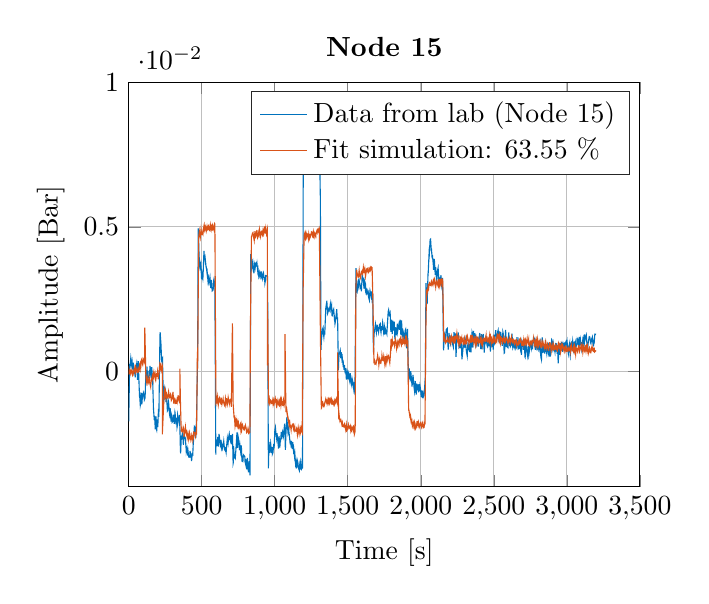
\begin{tikzpicture}

\begin{axis}[%
width=2.5556in,
height=2.02135in,
at={(1.011in,0.642in)},
scale only axis,
xmin=0,
xmax=3500,
xlabel={Time [s]},
xmajorgrids,
ymin=-0.004,
ymax=0.01,
ylabel={Amplitude [Bar]},
ymajorgrids,
axis background/.style={fill=white},
title style={font=\bfseries},
title={Node 15},
legend style={legend cell align=left,align=left,draw=white!15!black}
]
\addplot [color=mycolor1,solid]
  table[row sep=crcr]{%
0.05	-0.00173498670576727\\
6.3	0.000152892082111139\\
7.45	0.000136362267839293\\
14.25	0.00045912864125125\\
14.95	0.000426069012708127\\
17.9	0.00023728113391952\\
22.7	0.000355599804496093\\
25.85	5.54531769304395e-05\\
31.25	0.000294700488758348\\
36.05	1.36936461380827e-05\\
36.95	9.63427174976855e-05\\
44.3	-0.000182924144672469\\
44.55	-0.0002125038123168\\
51.7	0.00016246197458579\\
54.9	0.000265990811339559\\
59.05	-1.1536070382151e-05\\
60.45	-0.000298632844576471\\
65.25	0.000352989833822023\\
66.45	0.00017551182795722\\
73.2	-0.000771037536656027\\
73.95	-0.00075972766373375\\
79.25	-0.00118080293255253\\
81.3	-0.00112947350928891\\
85.3	-0.000737977908116597\\
90.25	-0.00114165337243186\\
94.35	-0.000771037536660302\\
96.3	-0.000863256500495166\\
100.5	-0.000738847898342235\\
103.7	-0.000791047311829718\\
107.25	-0.000988535092868392\\
112.15	-0.000925025806452595\\
117.65	-2.02359726333839e-05\\
120.35	-0.00032908250244823\\
124.85	0.000142452199407117\\
125.45	0.000141582209183616\\
129.8	-0.000312552688171042\\
138.55	-0.00013333470186154\\
139.4	2.3263538607321e-05\\
141.55	-0.000179444183775954\\
146.15	0.000187691691099806\\
147.6	0.000106782600188648\\
153.75	-0.000250783382209352\\
157.35	0.000141582209191429\\
162.3	-0.000178574193553868\\
162.9	-0.000108104985342902\\
169.65	-0.00130521153470688\\
175.15	-0.00169496715542827\\
177.05	-0.00154706881720762\\
182.05	-0.00201425356794935\\
186.9	-0.00156272864125633\\
191.8	-0.00204296324536166\\
191.85	-0.00204383323558623\\
196.5	-0.00166625747800672\\
199.15	-0.001937694428155\\
203.8	-0.00130521153470546\\
206.55	-0.00158273841642503\\
213.85	0.0011994903225773\\
215.1	0.00135173861192364\\
221.25	0.000911523558160002\\
225.05	0.00037038963831755\\
231.45	0.000449558748783482\\
236	-0.000704048289351167\\
237.9	-0.00109902385142994\\
242.9	-0.00065184887586546\\
245.95	-0.000724058064521305\\
248.35	-0.000583119648093697\\
250.8	-0.000639669012708663\\
255.15	-0.00107031417399561\\
259.3	-0.000870216422287129\\
265	-0.00137133079178575\\
266.2	-0.0013600209188656\\
272.3	-0.00104769442815672\\
272.9	-0.00106596422287701\\
279.25	-0.00146528973607508\\
283.9	-0.00127824183774017\\
287.65	-0.00160274819160583\\
291.15	-0.00174629657869652\\
292.95	-0.00151313919844077\\
295.35	-0.00156185865103317\\
297.9	-0.00176195640274236\\
304	-0.0017175869012771\\
306.4	-0.00150356930596834\\
311.6	-0.00182198572825136\\
316.65	-0.00141918025415926\\
317.6	-0.00144180000000879\\
323.45	-0.00184025552296524\\
327.1	-0.00161144809383522\\
331	-0.00193682443793897\\
332.1	-0.00190637478006117\\
335.05	-0.00151313919841946\\
339.3	-0.00162884789834655\\
343.65	-0.00175238651025289\\
348.55	-0.00151052922774646\\
353.9	-0.0027137257086931\\
355.5	-0.00284683421309317\\
360.3	-0.00223349110458705\\
361.35	-0.00237181955033314\\
366.5	-0.00217781173021159\\
369.75	-0.00213083225805626\\
374.25	-0.00254494760508343\\
376.1	-0.00242314897360352\\
381	-0.00223784105571916\\
388.95	-0.0023309300097889\\
390.7	-0.00254146764418656\\
390.95	-0.00251188797654116\\
394.25	-0.00279463479961456\\
399.3	-0.0026667462365605\\
402.5	-0.00281290459433414\\
405.6	-0.00273112551319166\\
410.6	-0.0029686328445802\\
417.7	-0.00297646275660063\\
420.15	-0.0027580952101669\\
420.45	-0.0027807149560143\\
427.7	-0.00295645298142908\\
430.6	-0.00310696129034049\\
435	-0.00286075405671617\\
438.7	-0.00288250381232977\\
442.45	-0.00244141876833161\\
442.85	-0.00247012844574462\\
449.6	-0.00190289481915293\\
451.4	-0.00191159472140576\\
456.9	-0.00219869149560842\\
459.2	-0.00231527018574233\\
464.6	-0.00160796813292556\\
471.95	0.000469568523958588\\
476.05	0.00494392825023376\\
481.65	0.0040321784946233\\
486.65	0.00360240332355383\\
487.8	0.00356934369501866\\
493.9	0.00373464183774425\\
494.15	0.00371202209190109\\
499.15	0.00317871808406985\\
501.45	0.00339534565005871\\
507.7	0.0032100377321644\\
508.8	0.00327789696970804\\
515.4	0.00417137693058756\\
516.25	0.00406001818180962\\
523.5	0.00382773079178556\\
524.45	0.00387471026393094\\
530.65	0.00357369364613086\\
531.15	0.00362241309872112\\
537.3	0.00335619608993235\\
538.3	0.00339273567937433\\
543.05	0.00311520879764836\\
546.2	0.0032256975561996\\
549.8	0.0030690993157439\\
556.3	0.00325701720430126\\
560.45	0.00297166041056905\\
561.25	0.00288205141741181\\
565.95	0.00316218826979089\\
568.1	0.00306648934506662\\
571.45	0.00278374252199605\\
578.2	0.0028202821114352\\
582.15	0.00315783831867585\\
583.95	0.00319785786901897\\
589.85	0.00291511104594129\\
589.95	0.00291685102639186\\
596.45	-0.00288337380254368\\
597.3	-0.00262933665688897\\
601.75	-0.00238051945260302\\
605.45	-0.00258235718476064\\
609.3	-0.00227612062560886\\
613.55	-0.00261106686216799\\
618.5	-0.00216824183774626\\
620.15	-0.00223436109483081\\
626.75	-0.00253624770284766\\
629.4	-0.00247795835777644\\
633.95	-0.00263977653961653\\
636.75	-0.00250318807430538\\
641.55	-0.00267109618767555\\
648.85	-0.00250318807428974\\
650.75	-0.00242227898338249\\
656.3	-0.00271633567938173\\
660.4	-0.00274765532750045\\
661	-0.00262411671556712\\
667.05	-0.00281203460409464\\
671.05	-0.00255625747797232\\
675.4	-0.00231440019548862\\
680.45	-0.00249361818182585\\
685.75	-0.00223784105572911\\
688.5	-0.00216650185729854\\
692.8	-0.00235093978494483\\
696.75	-0.00241705904207201\\
698.5	-0.00221348132946098\\
704.45	-0.00252667781038091\\
707.25	-0.00230831026393723\\
710.45	-0.00217346177908659\\
715	-0.00319570029321418\\
715.45	-0.00318526041051363\\
718.2	-0.00259714701856062\\
723.15	-0.00302605219941759\\
725.5	-0.00292513333333594\\
730	-0.00299386256107929\\
737.1	-0.00248404828933069\\
741.15	-0.0021203923753898\\
744.65	-0.00262324672533047\\
745.35	-0.00265456637344065\\
749.15	-0.00226133079177764\\
753.05	-0.00237268954059679\\
758.9	-0.00273199550342262\\
762.15	-0.00257974721405496\\
766.4	-0.00278158494622679\\
771.3	-0.00256930733137999\\
774.25	-0.0029851626588492\\
774.8	-0.00293644320625042\\
775.9	-0.00311218123166092\\
781.8	-0.00312871104593276\\
785.3	-0.00289120371456413\\
794.7	-0.0029477530791933\\
796.25	-0.00312523108506291\\
800.1	-0.00321049012708094\\
801.25	-0.00303562209190424\\
803.8	-0.00314350087978532\\
808.65	-0.00339753802542297\\
812.7	-0.00300430244380542\\
817.75	-0.00338274819157042\\
820.05	-0.00350280684259124\\
825.25	-0.00311653118279302\\
830.35	-0.00360546568913483\\
833.25	0.000269470772223113\\
836	0.00405914819157155\\
841.5	0.00384252062560685\\
844.85	0.00359283343110413\\
850.1	0.00377553137827427\\
855.15	0.00352149423264514\\
857.15	0.00338925571847036\\
862.25	0.00369027233623349\\
865.9	0.00358326353858907\\
869.75	0.00374508172043769\\
874.95	0.00377031143692541\\
876.45	0.00362328308894355\\
878.6	0.00371724203324\\
883.6	0.00346059491691797\\
885.7	0.00353193411534854\\
891.6	0.00323526744866919\\
892.7	0.00324483734113593\\
897.85	0.00345276500485917\\
900.4	0.00341883538609587\\
905.7	0.00323178748777089\\
907.65	0.00325005728248762\\
909.7	0.00345624496578019\\
915.4	0.00321264770283457\\
920.35	0.00334836617786785\\
922.85	0.00339621564024704\\
928.35	0.00316740821111133\\
929.55	0.00326919706742963\\
932.6	0.00304995953077487\\
936.5	0.00316305826001617\\
938.5	0.0033144365591415\\
950	0.00329268680349806\\
951.2	0.0030221198435573\\
956.4	-0.00336273841642587\\
960.9	-0.00244663870970604\\
965.15	-0.00280942463343585\\
966.65	-0.00280681466276853\\
972.15	-0.00249796813298921\\
973.35	-0.00255103753670873\\
977.15	-0.00283465434997189\\
981.95	-0.0026284666666708\\
983.95	-0.00286684398825621\\
988.15	-0.00280942463344153\\
992.55	-0.0025258078201329\\
995.6	-0.00266587624633238\\
1000.6	-0.00204731319646605\\
1004.6	-0.00194204437933755\\
1010.15	-0.00228221055721853\\
1012.45	-0.002147362072348\\
1013.9	-0.00234919980451984\\
1017.8	-0.00225698084069385\\
1024.95	-0.00261976676441797\\
1025.35	-0.00267457614858806\\
1029.7	-0.00224480097755979\\
1034.7	-0.00263977653961653\\
1038.7	-0.00237007956991242\\
1039.85	-0.00243271886609014\\
1044.75	-0.00210125259043642\\
1047.05	-0.00234919980450563\\
1053.75	-0.00210734252199919\\
1058.75	-0.00224828093842966\\
1061.7	-0.00206210303029017\\
1062.25	-0.00210038260019124\\
1067.7	-0.00181589579670564\\
1069.35	-0.00200381368528717\\
1072.75	-0.00272590557185132\\
1076.55	-0.0021725917888812\\
1083.05	-0.00158795835776679\\
1083.95	-0.00168017732160131\\
1090.8	-0.00212561231672445\\
1095.8	-0.00197945395896504\\
1098.55	-0.00221870127078709\\
1099	-0.00217607174977097\\
1106	-0.0025284177908258\\
1108.3	-0.00240487917889247\\
1113.3	-0.00264238651027249\\
1114.45	-0.00240922913001319\\
1120.45	-0.00269545591396642\\
1123.45	-0.00245272864124607\\
1128.05	-0.00272329560118401\\
1129.7	-0.00267544613879912\\
1135.55	-0.00295384301077312\\
1137.85	-0.00286510400782553\\
1142.9	-0.00322875992179483\\
1147.55	-0.00313915092863049\\
1148.8	-0.00333924868035744\\
1150.35	-0.00333141876834125\\
1153.55	-0.0030643317692931\\
1158.6	-0.00315568074290233\\
1162.2	-0.00334794858257048\\
1168.4	-0.00343842756599422\\
1172.4	-0.00314698084066371\\
1174.35	-0.00310783128056862\\
1178.85	-0.00339318807428235\\
1182.7	-0.0034071079179096\\
1185.6	-0.00320962013685282\\
1190.05	-0.00336708836753523\\
1194.55	0.00587481779080186\\
1195.95	0.00846303870966558\\
1204.65	0.00764611788856265\\
1208.55	0.00794017458456331\\
1209.5	0.00789841505375827\\
1216.25	0.00770092727268157\\
1216.65	0.007763566568865\\
1221.45	0.00804805337239892\\
1226.95	0.00767569755616826\\
1230.95	0.0078114160312584\\
1232.2	0.00773659687192102\\
1236.05	0.00798976402736465\\
1239.05	0.00796627429130191\\
1244.1	0.00759739843596385\\
1246.7	0.00791407487780199\\
1251.55	0.00765220782011689\\
1254.95	0.00770788719450088\\
1258.4	0.00785056559138192\\
1262.6	0.00771919706739831\\
1264.6	0.00786187546426796\\
1269.55	0.00766525767348476\\
1275	0.00788188523947504\\
1276.3	0.00774703675464146\\
1281.3	0.0081367923753323\\
1283.35	0.0080297835776964\\
1286.45	0.00779488621701213\\
1293.85	0.00780010615833825\\
1297.75	0.00798976402735613\\
1300.15	0.00787318533722506\\
1305.1	0.00806284320624578\\
1305.5	0.00807154310849861\\
1312.5	0.00592701720427904\\
1316.45	0.00074535542523968\\
1319.95	0.00110466138809109\\
1327	0.00145613743890359\\
1331.35	0.00151442678395775\\
1334.05	0.00128300938411208\\
1336.4	0.00118383049854352\\
1340.2	0.0014048080156801\\
1342.4	0.00126560957966895\\
1349.35	0.00217648934509107\\
1356.7	0.00242791651996477\\
1356.75	0.00242791651995909\\
1361.5	0.00199379139783283\\
1364.1	0.0020277210165677\\
1366.3	0.00216604946234789\\
1372.6	0.00209906021502385\\
1378.8	0.00225478846530401\\
1380.7	0.00232438768325843\\
1383.8	0.00213994975564624\\
1389.3	0.00228523812316049\\
1392.4	0.00192419217985568\\
1394.25	0.00192071221896023\\
1397	0.00205904066474041\\
1403.55	0.00214777966767379\\
1408.35	0.00184154310851065\\
1409	0.00185111300097739\\
1412.45	0.00164492531769334\\
1416.05	0.00175019413486731\\
1423.1	0.00207035053760657\\
1424.1	0.0021529996089516\\
1428.55	0.00179195366565815\\
1430.45	0.00186851280543757\\
1435.65	3.54434017442173e-05\\
1439	0.000468698533764578\\
1441.75	0.000603547018626582\\
1448.35	0.000726215640300509\\
1452.6	0.000446948778155237\\
1455.35	0.000656616422346101\\
1459.95	0.000423459042015753\\
1462.25	0.00048696832843298\\
1467.25	0.000243371065558412\\
1469.65	0.000286000586534746\\
1474.7	5.19732160473296e-05\\
1477.35	0.000210311436935132\\
1482.1	-6.8085434996229e-05\\
1484.05	0.000110262561061711\\
1489.05	-0.00015334447700574\\
1490.5	-0.000289932942341045\\
1495.65	1.19536657354757e-05\\
1498.4	-4.37257086428333e-05\\
1501.25	-0.000282973020504673\\
1506.4	-9.59251221825386e-05\\
1511.45	-0.000302982795663445\\
1513.85	-0.000358662170092922\\
1516.4	-6.63454546138698e-05\\
1518.95	-0.000168134310858284\\
1526.1	-0.000463060997098447\\
1527.1	-0.0004865507331413\\
1530.6	-0.000272533137852443\\
1535.3	-0.000381281915961651\\
1540.9	-0.000616179276606121\\
1542.95	-0.000530050244325855\\
1547.95	-0.000717968132998334\\
1549.15	-0.000687518475136165\\
1555.8	0.00352062424243123\\
1556	0.00357021368523824\\
1562.6	0.00275590283474295\\
1564.05	0.00274285298135234\\
1570.5	0.00303429970672547\\
1572.6	0.00296296050829206\\
1576.65	0.00321525767349905\\
1578.3	0.00313608856304946\\
1583.55	0.00293512082105458\\
1585.3	0.00297949032260654\\
1592.5	0.00281419217980848\\
1593.25	0.00276982267833042\\
1598.65	0.00332226647113494\\
1602.55	0.003238747409576\\
1606.95	0.00309867898336798\\
1607.4	0.00310998885626823\\
1611.15	0.00286030166172574\\
1614.9	0.00307779921794982\\
1619.75	0.00287074154443481\\
1622.15	0.00295165063534633\\
1625.95	0.00265324398819936\\
1631.1	0.00286552160313427\\
1632.9	0.00269152355812885\\
1639.85	0.00275938279566112\\
1641.8	0.00257929481911284\\
1647.85	0.00246358611926958\\
1651.55	0.00277069266857843\\
1652.1	0.00279331241441874\\
1659.05	0.00262018435972387\\
1661.25	0.00276199276631993\\
1665.9	0.00250012570867462\\
1670.9	0.0026706437927448\\
1673.8	0.00127430948186494\\
1676.15	0.000655746431995757\\
1680.6	0.00139871808410313\\
1681.3	0.00132041896386177\\
1687.9	0.00157358611921446\\
1689.6	0.00163187546429705\\
1695.5	0.00136043851416795\\
1696	0.00134129872923446\\
1701.25	0.00161447565978001\\
1704.85	0.00139001818178208\\
1705.75	0.00152921661779325\\
1711.1	0.0013569585532327\\
1716.95	0.00161099569890162\\
1723	0.00164927526880271\\
1724.15	0.00146309736070585\\
1727.8	0.00133955874873842\\
1732.25	0.00156227624629146\\
1733.9	0.00142655777120987\\
1738.95	0.00169277478003274\\
1740.5	0.00163796539582856\\
1745.65	0.00135086862168983\\
1751.3	0.00152399667641881\\
1753.4	0.00128909931568338\\
1756.3	0.00129170928633648\\
1758.65	0.00144830752687604\\
1767.65	0.00128996930590866\\
1769.65	0.00149441700874782\\
1769.85	0.00147875718469273\\
1776.8	0.00206861055720715\\
1779.85	0.00212776989246387\\
1784.3	0.00196247174973402\\
1790.2	0.00203555092864641\\
1791.75	0.00181979335288994\\
1795.2	0.0013613085043705\\
1800	0.00179108367546697\\
1804.2	0.00128474936460243\\
1807.85	0.0017510641251608\\
1812.85	0.00141263792768492\\
1818.15	0.0017188744867685\\
1821.25	0.00124820977516329\\
1823	0.00111684125119105\\
1828.05	0.00150137693061261\\
1828.9	0.00149963695014499\\
1834.55	0.00124559980452724\\
1839.7	0.00165014525905072\\
1841.5	0.00138044828934945\\
1845.15	0.00148658709677144\\
1850.3	0.00163013548381237\\
1854.95	0.00143438768322604\\
1858.1	0.00174149423263154\\
1858.45	0.00178412375365333\\
1863.5	0.00126125962849706\\
1868.15	0.00175802404686075\\
1872.75	0.00132824887585521\\
1873.45	0.00122037008799972\\
1879	0.00138305826003099\\
1881	0.0013360787878714\\
1885.55	0.00109161153470333\\
1889.05	0.00115251085045039\\
1892.95	0.00141089794718888\\
1896.45	0.00145526744866693\\
1902.35	0.00112641114369759\\
1903.95	0.000796684848497264\\
1908.8	0.00147092727269929\\
1909.7	0.00132476891493134\\
1916.2	-0.000374321994085491\\
1921.25	9.89526881784997e-05\\
1923.9	-0.00016465435001968\\
1928.2	-0.000256003323532275\\
1931.45	5.86373419260433e-06\\
1931.85	-2.28459432076167e-05\\
1939.2	-0.000448271163228847\\
1940.2	-0.000532660215035813\\
1946.3	-0.000152474486746351\\
1946.85	-0.000127244770213142\\
1953.95	-0.000558759921851143\\
1957.35	-0.000687518475113433\\
1961.25	-0.00041956148581157\\
1962.5	-0.000338652394888672\\
1968.4	-0.000807577126145625\\
1969	-0.000781477419375773\\
1973.05	-0.000429131378261255\\
1977.75	-0.000657938807396966\\
1979.85	-0.000454361094783085\\
1984.55	-0.000726668035222741\\
1989.45	-0.000446531182755547\\
1994.3	-0.000694478396847484\\
1995.5	-0.000537010166173593\\
1998.2	-0.000617049266888256\\
2003.05	-0.000885876246369932\\
2005.55	-0.000665768719492726\\
2010.1	-0.000923285826108247\\
2014.05	-0.000674468621700078\\
2016.8	-0.000899796089946031\\
2022.85	-0.000836286803500383\\
2027.7	-0.000456101075273441\\
2030.55	-0.000520480351881847\\
2035.05	0.00269848348001639\\
2035.85	0.00305256950151325\\
2041.85	0.00233830752686295\\
2043.85	0.00234961739975753\\
2049.5	0.00338055581619479\\
2049.9	0.00330921661773864\\
2057.15	0.00410960762466353\\
2058.55	0.00406436813293745\\
2064	0.00456374252201677\\
2067.05	0.00457766236561562\\
2071.9	0.00418094682305714\\
2072.85	0.00425489599217209\\
2077.8	0.00391385982404309\\
2079.6	0.00403043851424237\\
2086.7	0.00362676304989301\\
2087.45	0.00351540430106817\\
2092.35	0.00389124007818574\\
2094.05	0.00378075131964871\\
2098.85	0.0033396662755667\\
2102	0.0036006633431061\\
2108.65	0.00310041896375034\\
2109.1	0.00307605923745946\\
2114.55	0.0034945245356159\\
2118.75	0.00358413352882572\\
2123.55	0.00310737888563217\\
2123.85	0.00307344926685182\\
2125.55	0.00324222737043733\\
2133.75	0.00315522834796021\\
2138.3	0.00332313646134318\\
2141.75	0.00298732023457725\\
2149.15	0.00323526744865782\\
2153.05	0.00181109345064279\\
2156.05	0.000724475659815843\\
2160.65	0.00117252062558074\\
2162.95	0.00127343949166808\\
2169.3	0.00112380117300469\\
2174.1	0.0014413476050283\\
2181	0.00148484711626971\\
2182.45	0.00119514037142672\\
2182.7	0.00120645024433835\\
2187.95	0.000747965395875738\\
2189.95	0.000877593939340574\\
2192.75	0.00132563890510547\\
2199.15	0.00109596148575584\\
2203	0.000977642815270852\\
2204.65	0.00107334174001786\\
2206.8	0.00122124007816247\\
2213.05	0.00121167018572983\\
2215.5	0.000999392570851756\\
2222.7	0.00084366432065118\\
2226.75	0.0013004091886689\\
2227.85	0.00135260860212903\\
2230.15	0.00100635249259717\\
2236.8	0.00131345904192309\\
2241.2	0.000497408211125011\\
2241.6	0.000523507917877808\\
2247.3	0.00125429970671753\\
2251.15	0.00103245219935566\\
2256.1	0.0013491286412279\\
2256.25	0.0013265088953876\\
2262.65	0.000815824633425069\\
2264	0.000821914565030474\\
2270.2	0.00105420195506163\\
2272.75	0.000797554838694134\\
2277.6	0.00102288230694009\\
2278.4	0.000934143304018073\\
2281.7	0.000410409188664931\\
2287.75	0.000707945845592306\\
2292.9	0.00102810224829747\\
2294.4	0.000822784555284173\\
2296.65	0.00104289208215569\\
2301.55	0.000905433626572361\\
2306.55	0.00106551182795621\\
2307.85	0.000921093450661561\\
2312.65	0.000678366177978174\\
2318.1	0.000527857869015602\\
2322.55	0.000966332942342163\\
2323.05	0.000975902834814593\\
2326.5	0.000721865689196841\\
2330.65	0.000955023069481697\\
2335.65	0.000667926295229299\\
2342.1	0.0010289722385739\\
2343.7	0.000651396480994396\\
2344.75	0.000784504985411522\\
2350.95	0.00133955874879527\\
2352.9	0.00129344926688368\\
2356.3	0.000818434604123661\\
2361.3	0.00139610811341023\\
2365.3	0.00098025278589553\\
2370.25	0.00131606901263304\\
2374.15	0.000969812903209188\\
2374.8	0.000946323167143603\\
2378.2	0.00113076109481831\\
2383.1	0.000953283088934498\\
2388.5	0.00118470048879722\\
2389	0.00113424105574787\\
2393.9	0.000854104203348888\\
2397.4	0.00109509149559878\\
2403.7	0.00132302893448646\\
2410.2	0.000763625219919462\\
2415.05	0.00128213939393228\\
2418.45	0.000862804105613083\\
2419.8	0.00075927526884989\\
2424.6	0.00125516969687461\\
2427.95	0.00126473958939251\\
2432.95	0.000797554838665712\\
2434.4	0.000647916520030739\\
2439.5	0.00105420195501048\\
2440.6	0.000942843206248156\\
2445.35	0.00116034076242677\\
2447.95	0.00111771124142201\\
2454.1	0.000887163831881213\\
2457.55	0.000848884261917607\\
2462.7	0.00101853235577956\\
2463.9	0.00109335151510273\\
2468.4	0.000861064125099995\\
2472.7	0.00110292140762064\\
2476.45	0.000685326099712225\\
2477.7	0.000753185337221754\\
2481.5	0.00115860078204442\\
2488.65	0.000836704398871652\\
2492	0.00109857145653401\\
2496.25	0.000747965395921216\\
2499.6	0.00115338084064157\\
2504.65	0.00102897223847727\\
2506.7	0.00126995953076126\\
2507.95	0.00112119120232315\\
2513	0.00142655777124397\\
2515.05	0.00131171906156347\\
2520.3	0.00116556070380121\\
2524.35	0.00118731045943897\\
2526.7	0.00137783831865086\\
2529.8	0.00142829775164906\\
2535.55	0.0010054825024458\\
2536.45	0.00107421173020335\\
2540.55	0.00138218826982844\\
2545.6	0.0010994414466456\\
2546.8	0.00135695855320997\\
2551.45	0.00118905043986112\\
2557.65	0.000880203910061897\\
2558.55	0.00104376207232981\\
2562.1	0.00136130850433638\\
2565.95	0.00126734956006268\\
2571	0.000625296774179065\\
2573.5	0.00063660664711912\\
2580.6	0.0014178578690025\\
2580.8	0.00143351769305761\\
2585.75	0.000835834408629318\\
2589.4	0.00112206119255981\\
2593.25	0.0008401843596932\\
2597.05	0.000816694623695824\\
2602.3	0.00134129872919467\\
2602.95	0.0012812694036672\\
2609.15	0.000868894037133222\\
2610.15	0.00102027233626992\\
2613.55	0.000850624242476172\\
2619.5	0.000907173607022929\\
2624.65	0.00130562913006038\\
2624.95	0.0012751794722039\\
2630.3	0.000800164809449555\\
2634.15	0.000850624242464806\\
2639.2	0.00107334173997807\\
2641.95	0.000896733724353643\\
2646.85	0.00107856168134113\\
2647.05	0.00105072199414913\\
2650.85	0.000782765004921165\\
2654.6	0.000820174584574229\\
2658.65	0.00118122052782788\\
2661.8	0.000990692668621673\\
2666.85	0.00077232512218367\\
2670.9	0.000792334897348118\\
2672	0.0010133124144506\\
2681.05	0.000785374975551534\\
2682.2	0.000955023069373701\\
2684.3	0.0010202723362415\\
2689.1	0.000567877419401341\\
2691.35	0.000775805083084793\\
2694.15	0.00103506216999172\\
2699.95	0.00095154310859194\\
2704.1	0.000742745454660465\\
2709.1	0.00107334174002922\\
2713.15	0.00049914819174042\\
2714.8	0.000480878396958317\\
2718	0.000814084653031344\\
2721.8	0.000926313391973466\\
2728.15	0.000612246920936255\\
2731.7	0.00051741798639747\\
2735.45	0.00080190478991149\\
2736.5	0.000884553861296322\\
2740.4	0.000588757184813826\\
2743.85	0.000712295796803986\\
2749.65	0.00105246197463381\\
2750.3	0.000983732746864877\\
2757.05	0.000787984946147804\\
2762.75	0.00106029188672388\\
2764.6	0.000759275268866946\\
2765.2	0.00080364477032796\\
2772.2	0.00117165063533271\\
2778.05	0.0011429409580746\\
2779.75	0.000877593939573637\\
2781.25	0.000968072922866631\\
2783.85	0.000746225415561602\\
2788.85	0.00102810224834862\\
2794	0.000821914564950899\\
2798.7	0.000942843206350477\\
2800.25	0.000776675073429448\\
2803.8	0.0007375255130814\\
2808.05	0.000932403323692557\\
2813.5	0.000781895014758408\\
2815.25	0.000962852981514939\\
2817.25	0.0010072224829191\\
2822.2	0.000490448289305695\\
2826.4	0.000399969305989956\\
2831.35	0.00109857145647717\\
2832.1	0.00117078064507901\\
2837.25	0.000660966373438404\\
2839.75	0.000666186314744632\\
2844.8	0.000892383773272706\\
2849.05	0.000612246920936255\\
2853.5	0.000854974193625332\\
2855.25	0.000946323167240248\\
2860.85	0.000674886217145246\\
2862.75	0.000608766960023752\\
2867.4	0.000859324144700579\\
2873.35	0.000663576344165417\\
2875.5	0.000833224437964838\\
2876.9	0.000995042619753764\\
2882.05	0.000524377908279305\\
2886.65	0.000524377908165619\\
2888.3	0.00079929481918449\\
2890.35	0.00062007683283305\\
2896.5	0.0011046613880371\\
2897.85	0.00109683147601523\\
2901.8	0.000810604692084743\\
2906.95	0.000975032844589316\\
2912.45	0.0007601452592116\\
2914.6	0.000803644770305215\\
2919	0.000666186314721887\\
2923.75	0.000983732746842145\\
2926.6	0.000680976148671075\\
2930.2	0.000961982991306704\\
2934	0.000602677028350138\\
2936.8	0.000896733724336587\\
2940.85	0.000270340762473967\\
2943.15	0.000497408211233008\\
2946.15	0.00086367409584405\\
2952.4	0.000568747409558423\\
2956.7	0.000972422873873668\\
2960.1	0.000754925317564326\\
2963.15	0.00100200254137413\\
2966.15	0.000998522580677633\\
2971.1	0.00067227624647509\\
2971.45	0.000699245943430432\\
2975.25	0.000941973216062666\\
2982.95	0.000788854936412883\\
2984.7	0.000995912609939253\\
2989.4	0.00072534565012071\\
2993.3	0.00103158220921565\\
2998.85	0.00106638181814739\\
3000.65	0.000956763049886789\\
3002.1	0.00101679237542562\\
3007.75	0.000700115933615922\\
3010.55	0.00060963695018651\\
3015.7	0.000899343694915802\\
3019.5	0.000987212707686425\\
3023	0.000543517693087747\\
3023.15	0.000538297751724676\\
3028	0.000953283089042509\\
3031.1	0.00098808269806519\\
3035.05	0.000827134506450389\\
3039.9	0.00104202209195314\\
3044.85	0.000754055327560732\\
3046.6	0.000712295796781254\\
3051.7	0.00103158220913607\\
3054.15	0.000780155034160054\\
3059.2	0.00100983245369157\\
3060.25	0.00102897223860232\\
3061.85	0.000834094428241283\\
3069.9	0.000949803128039051\\
3071.7	0.00113076109473874\\
3074.9	0.00109857145643169\\
3079.75	0.000886293841655936\\
3084.65	0.00119253040086456\\
3088.95	0.000943713196581444\\
3093.15	0.00108465161280442\\
3095.65	0.000915873509258702\\
3096.8	0.0010150523948159\\
3102.3	0.000753185337375228\\
3104.2	0.000815824633493278\\
3110.75	0.00116382072332222\\
3112.1	0.00118209051803611\\
3117.9	0.000857584164261391\\
3120.05	0.000995912610041574\\
3122.85	0.00127430948185925\\
3126.55	0.00111597126089187\\
3133.55	0.00123689990234831\\
3133.7	0.00121689012718385\\
3139.65	0.000811474682361188\\
3142.6	0.000785374975636799\\
3148.3	0.00107073176929084\\
3148.4	0.00105507194524712\\
3153.7	0.00119862033218575\\
3157.5	0.0011847004886949\\
3162.9	0.000985472727338177\\
3164.95	0.000959373020613802\\
3169.9	0.00111684125116832\\
3175.2	0.00118818044976657\\
3177.9	0.00100374252198386\\
3182.75	0.000859324144643736\\
3183.8	0.00109422150531097\\
3186.65	0.000941103225831699\\
3191.9	0.00128735933536923\\
3200	0.00127952942323369\\
};
\addlegendentry{Data from lab (Node 15)};

\addplot [color=mycolor2,solid]
  table[row sep=crcr]{%
0.05	1.94720339494414e-05\\
0.1	-0.000117832170262541\\
1.1	8.44317864917298e-05\\
10.7	-8.36735461168511e-05\\
13.75	4.17764286027361e-05\\
15.85	6.18322428193571e-05\\
21.45	-7.40676008365354e-05\\
24.65	-0.000117534577328753\\
25.7	-1.98934246637055e-05\\
30.7	-9.68007645580985e-05\\
35.8	4.57535169708135e-05\\
38.05	-5.0076110474441e-09\\
42.05	0.000124378020385546\\
46	2.62298204143708e-06\\
48.2	0.000153672106391572\\
51.7	9.1201775099476e-05\\
56.7	-2.95488483945772e-05\\
59.75	-4.00002491688651e-05\\
63.55	9.09840478207643e-05\\
67.85	1.60793493128588e-05\\
72.95	0.000172442404921685\\
74.45	0.000112878276815256\\
79.3	0.000244489212548565\\
82	0.000114998285358298\\
87.5	0.000397896856352938\\
90.8	0.00043329065495288\\
95.75	0.000229612171218556\\
96.15	0.000223292562968807\\
102.25	0.000404266937092886\\
109.95	0.000288515729587103\\
110.15	0.00151171520367997\\
110.7	0.00141661137535524\\
117.7	-0.000260681304450714\\
118.25	-0.000210920496111716\\
121.3	-0.000364547249331632\\
126.15	-0.000217684916363417\\
131.9	-0.000435447209170464\\
133.15	-0.000420239600403702\\
139.95	-0.000193173028143035\\
140.5	-0.000208899539269846\\
143.9	-0.000400507020629376\\
150.35	-0.00054401037843101\\
154.55	-0.000281261192984764\\
154.9	-0.000331258776562288\\
161.25	-0.000166599771668133\\
166	-0.000294085321214549\\
167.6	-0.000141779231930391\\
171.05	-4.80430744172365e-05\\
172.75	-0.000175787155471756\\
179.85	-6.16678105960493e-05\\
182.05	-0.000274879127641866\\
184.85	-0.000317846044258887\\
191.45	-6.28727079639709e-05\\
192.6	-0.000192495707276921\\
197.6	-3.73079738625074e-06\\
202.6	-0.000281260576546612\\
206.05	-6.63067033180263e-05\\
206.8	-0.000122422008110081\\
213.75	0.000286422750828908\\
213.95	0.00028535227544628\\
218.2	9.51029633972894e-05\\
221.8	0.00018588750290461\\
225.8	3.38974894431236e-05\\
230.05	0.000139072667353009\\
230.15	-0.0021834461774553\\
241.35	-0.000934794462309441\\
243.35	-0.000707308029974105\\
244.25	-0.000663872905581446\\
247.65	-0.000836029708472944\\
251.05	-0.00070406822825994\\
256.05	-0.000928084198575777\\
259.25	-0.000790386706345184\\
264	-0.000913152204167815\\
267.75	-0.000933801602272113\\
272.75	-0.000711180452341481\\
273.1	-0.000699281868551218\\
279.7	-0.000921941362534299\\
280.8	-0.000920239355606969\\
286.9	-0.00079687194070597\\
287.7	-0.000810665748962323\\
291.9	-0.00100763960802124\\
295.9	-0.00096429031043299\\
302.35	-0.000751401695126599\\
302.85	-0.000714531151699898\\
308.8	-0.00110582452932577\\
310.6	-0.0011089144747397\\
316.2	-0.000954321876614625\\
317.8	-0.00097490319225679\\
322.1	-0.00111665214062387\\
326	-0.00111105252480103\\
330.1	-0.000990055169283773\\
332.4	-0.00105810733558456\\
338.5	-0.000850367544685275\\
340.55	-0.000854894045482893\\
345.5	-0.00104894383315922\\
349.95	-0.00109019875983864\\
350.15	8.683324488378e-05\\
354	-0.0010115153905544\\
359.55	-0.00209350607684992\\
361.4	-0.00197021854374234\\
366.4	-0.00209898888250246\\
371.1	-0.00205738548335772\\
373.45	-0.00193489961940441\\
376.1	-0.00197651380297221\\
379	-0.00227165063369173\\
388.3	-0.00193277516982193\\
390.6	-0.00208747477012733\\
394.45	-0.0021639887435611\\
396.2	-0.00202269662064745\\
398.3	-0.00211032441903011\\
400.95	-0.00228311881267183\\
405.9	-0.00217779652181009\\
408.55	-0.00236027118999587\\
416.1	-0.00214631585239101\\
418.6	-0.00228143608871852\\
420.55	-0.00223492588754031\\
425.95	-0.00239648164253078\\
428.7	-0.00235055492891643\\
432.2	-0.00219935430682018\\
435.9	-0.00227128917304892\\
439.05	-0.00240339487393396\\
442.5	-0.00231086988780321\\
445.65	-0.00210592212043391\\
454.1	-0.00213265803340478\\
456.95	-0.00226902089152081\\
458.2	-0.00224747563006768\\
461.5	-0.00210202102352606\\
464.65	-0.00219328561492738\\
470.15	0.000682233414829416\\
471.95	7.64456713413025e-05\\
479.15	0.00465001366543687\\
479.35	0.00464419417898383\\
483.75	0.00485117451688362\\
490.15	0.00463922907005593\\
493.25	0.00480685537896395\\
495.2	0.00491416432029641\\
499.8	0.00473532279464376\\
503.75	0.00473078268106415\\
508.8	0.00486999635237309\\
510	0.0048172836093624\\
515.7	0.0050482112746998\\
516.8	0.00507215844618966\\
520.25	0.00489713046824667\\
525.5	0.00500201940186646\\
530.55	0.00485329315638875\\
534.8	0.00497647469877154\\
536.1	0.00488248466333358\\
539.45	0.0049060297972651\\
545.5	0.00505861019204143\\
547.05	0.00506045641846707\\
550.35	0.00488966063363132\\
555.55	0.0048676164718265\\
559.45	0.00506901504673061\\
564.45	0.00493066415793489\\
566.5	0.00504922450868491\\
570.2	0.00506969806677907\\
573.7	0.00489704637891053\\
575.95	0.00490875379369624\\
577.1	0.00503076256600853\\
583.55	0.00490233620203208\\
588.6	0.00510955369502303\\
590.1	0.00509463638524673\\
597.3	-0.00102374104794122\\
600.85	-0.000935890470113443\\
603.7	-0.00106768909412421\\
605	-0.0010203151622994\\
608.75	-0.000875371561523037\\
613.75	-0.00115547898237482\\
619.4	-0.000959456495332305\\
622.1	-0.00092245318737764\\
626.3	-0.00107917779741245\\
629.35	-0.00110556889044058\\
633.5	-0.000914324122202487\\
634.45	-0.000970274428535933\\
638.5	-0.00113608497425692\\
646.2	-0.00095791266687949\\
648	-0.00110135758760889\\
648.9	-0.00103706718879647\\
655.4	-0.00117983437676899\\
657.05	-0.00119421909868971\\
662.1	-0.000958263074518531\\
665.55	-0.00113295537924261\\
670.6	-0.000929656986262321\\
671.05	-0.000963870072960546\\
675.55	-0.00114017852067001\\
678.4	-0.00106445701791694\\
681.3	-0.000904741282309383\\
688.9	-0.00111327542761225\\
690.8	-0.00100322495342507\\
696.6	-0.00097388396144418\\
700.3	-0.00112565410660414\\
700.8	-0.00105603569709326\\
703.05	-0.00123494529687588\\
710.15	0.00165433244258165\\
715.25	-0.00115264214489509\\
715.3	-0.00114114697819429\\
721.8	-0.00162062179563915\\
723.25	-0.00153191355714438\\
728.2	-0.00189599130638484\\
733.6	-0.00169823862603275\\
736.95	-0.00191431240331993\\
740.35	-0.0017684028090708\\
743.35	-0.00187829671923865\\
747.6	-0.00174534063478261\\
750.8	-0.00187696783671951\\
752.5	-0.00182362739795205\\
756.6	-0.00196506346186618\\
764.45	-0.00183527021680044\\
766.9	-0.00198016735287228\\
768.05	-0.00204552055762542\\
773.1	-0.0018793141136183\\
774.7	-0.00200735854162946\\
779.4	-0.00186099995069999\\
781.8	-0.00189957335549666\\
788.5	-0.00202891054167145\\
791.95	-0.00203401055556378\\
796.05	-0.00187284875296424\\
797.45	-0.00198798751835396\\
799.8	-0.00188229550321187\\
804.1	-0.00196642823103222\\
807.35	-0.00212801186988974\\
812.65	-0.00209921166252432\\
817.35	-0.00197302319734414\\
818.75	-0.002008331861911\\
821.5	-0.00215277042331644\\
830	-0.00211738486162756\\
833.25	0.00143467959583587\\
840.55	0.00467219313701355\\
840.7	0.00464751962227226\\
847.5	0.00477706672261407\\
850.95	0.00480187896994167\\
855.2	0.00464564081588161\\
859.5	0.00452759470275659\\
862.75	0.00473637300492252\\
864.35	0.00485077076998278\\
869.2	0.00464128062764923\\
870.6	0.00465129568310876\\
877.25	0.0048685116781852\\
878.35	0.0048654194566639\\
883.15	0.00462368545417486\\
885	0.00465020868410317\\
890.3	0.00481361642804325\\
892.65	0.00475292813024431\\
895.4	0.00491298184773717\\
902.95	0.0046716798131879\\
906.5	0.00481807264975715\\
910.8	0.00484576619141733\\
913.7	0.00473496912650588\\
916.65	0.00470182727299294\\
920.3	0.00488971375119624\\
924.95	0.00476489509469039\\
929.1	0.00488883936926631\\
931	0.00501845167385284\\
935.95	0.00477186604079961\\
938.85	0.00493790298924317\\
943.35	0.00476011103602928\\
949.15	0.0049040455459023\\
950.15	0.000203121279266734\\
951.2	0.00208261766236604\\
957.25	-0.00104683296805988\\
962.25	-0.00093984126476773\\
965.9	-0.00113343253053324\\
966.2	-0.0011292826228173\\
971.25	-0.000994774514670882\\
973.9	-0.00100357139698181\\
978.1	-0.00111646560746511\\
981.4	-0.00111559205363262\\
986.35	-0.000992308186367117\\
989.1	-0.00113953676612282\\
993.6	-0.00101436672847152\\
996.35	-0.00111416888604076\\
1002.3	-0.000994058639589319\\
1003.95	-0.000945891671853438\\
1008.9	-0.00109858739158057\\
1010.5	-0.00095867505155104\\
1015.5	-0.00117757909090501\\
1021.25	-0.00101765592409162\\
1024.65	-0.00113990686217597\\
1028.1	-0.00117060267029262\\
1031.05	-0.00104792947807958\\
1034.2	-0.00113478935822789\\
1039.05	-0.000988116722224105\\
1042.35	-0.00116888315439063\\
1046.25	-0.000989774459870053\\
1047.45	-0.00103131709041346\\
1051.7	-0.00117245552537012\\
1054.75	-0.00118116159204627\\
1059.6	-0.000992902831139696\\
1064.55	-0.00117030927859311\\
1069.05	-0.00103257972787958\\
1070.15	0.00128665645142971\\
1076.55	-0.00141419477625383\\
1079.3	-0.00128819313141973\\
1083.8	-0.00144483453501805\\
1084.4	-0.00140721382056978\\
1090.6	-0.00164820412045368\\
1091.75	-0.00162961858125469\\
1097.8	-0.00185811590148792\\
1101	-0.00167283171857727\\
1106.05	-0.00194218837282314\\
1106.95	-0.00185651385377201\\
1112	-0.00203157982015986\\
1113.4	-0.00195902977719337\\
1120.8	-0.0018393663666905\\
1123.5	-0.00182697525790502\\
1127.45	-0.00197368799722747\\
1129.75	-0.00189480893443817\\
1135.25	-0.0020289245282475\\
1137.35	-0.00196066436599593\\
1138.85	-0.00207122809451203\\
1144.8	-0.00207592593630235\\
1149.85	-0.00197589493489057\\
1150.65	-0.00198966213907831\\
1155.2	-0.00220376867623515\\
1157.65	-0.00210993280459118\\
1160.8	-0.00195470707058506\\
1167.05	-0.00216990310017157\\
1172.05	-0.0019850051703092\\
1172.45	-0.00197468348246283\\
1176.5	-0.0021100899312117\\
1180.8	-0.00196008767141431\\
1187.05	-0.00210125046445762\\
1188.2	-0.00211889813994079\\
1194.55	0.0028699970691349\\
1201.25	0.00470463637321619\\
1205.85	0.00478527520952002\\
1208.8	0.0045827159322945\\
1210.15	0.00456827128986671\\
1214.45	0.004777389407049\\
1219.15	0.00465657662219561\\
1221.45	0.00476336600769275\\
1226.75	0.00474235980499615\\
1231.1	0.00460474750417266\\
1232.9	0.00475059115068345\\
1237.55	0.00462822292279142\\
1239.55	0.00475448635669859\\
1242	0.00463252698464284\\
1246.6	0.00468942889451091\\
1251.6	0.00483034892392059\\
1254.8	0.00482087325101385\\
1260.2	0.00465138162215957\\
1262.05	0.00463772592751402\\
1264.9	0.00482183327649878\\
1269.9	0.00468943395884088\\
1271.55	0.00478448468027397\\
1280.9	0.00466047142574872\\
1283	0.00482186562884993\\
1283.65	0.00476949270031684\\
1290.15	0.00489769932359391\\
1293.5	0.00491706493504679\\
1295.15	0.00479873807803839\\
1298.5	0.00483537073310779\\
1304.7	0.00495943051978333\\
1305.25	0.00494520485597257\\
1312.5	0.00131276370160495\\
1319.1	-0.0012829649267216\\
1321.1	-0.00126703635176255\\
1326.95	-0.00105285645813287\\
1327.7	-0.00105017676116251\\
1332.75	-0.00120468778606102\\
1335.15	-0.00122185742155318\\
1341.9	-0.00110284841251235\\
1342.15	-0.00112112234980092\\
1348.95	-0.000968233359882995\\
1349.45	-0.000985235040836523\\
1354.85	-0.00108087245525658\\
1357.8	-0.00101932814210705\\
1359.55	-0.00112142447446057\\
1366.9	-0.000985915544460252\\
1368.1	-0.00108718694562426\\
1373.1	-0.000995866082480771\\
1375.6	-0.00109432468958738\\
1380.65	-0.00097262097458383\\
1385.35	-0.00107503701000171\\
1388.05	-0.000987671376890915\\
1392.4	-0.00113811178169234\\
1396.35	-0.00114086906563129\\
1397.4	-0.00104881101768748\\
1403.75	-0.00114928839504513\\
1406.9	-0.0010513935585174\\
1409.15	-0.00113443780184846\\
1414.15	-0.00101517039381484\\
1418.15	-0.00108711187766794\\
1423.1	-0.000956759919895268\\
1430.1	-0.00111339658490571\\
1430.15	0.000655474977925405\\
1430.55	0.000313204281399737\\
1437.7	-0.00150845854661569\\
1439.8	-0.00145353391646886\\
1444.5	-0.00168616171134493\\
1445.55	-0.00161227351849149\\
1447	-0.0017393637755405\\
1453.1	-0.00168515396720929\\
1459.95	-0.0018585893427306\\
1463.1	-0.00179727830082685\\
1464.35	-0.00190886294274447\\
1473.2	-0.00192796609175209\\
1474.65	-0.00183626200392848\\
1476.95	-0.00181660888313375\\
1482.1	-0.0019389915364678\\
1485.9	-0.00203197937191805\\
1489.25	-0.00189117977816558\\
1490.2	-0.00185126424562055\\
1494.25	-0.00205072492828537\\
1497.8	-0.00201928414421922\\
1504.2	-0.00184532239472734\\
1509.2	-0.00196924984980774\\
1516.9	-0.00188252483524181\\
1518.65	-0.00199116121526381\\
1520.9	-0.00206671530796796\\
1524.85	-0.00196638794716368\\
1527.15	-0.00203719054115949\\
1532.4	-0.00195194996833925\\
1536.15	-0.00192062887005487\\
1537.8	-0.00202780200799799\\
1541.35	-0.00195774276187305\\
1545.1	-0.00218642463418655\\
1550.7	-0.00207868816392957\\
1555.8	0.00291384364009965\\
1560.4	0.00351641445966836\\
1563.2	0.00341970090422808\\
1570.15	0.00326367805791827\\
1573.25	0.0032594231632443\\
1577.45	0.00347360999692841\\
1578.05	0.00349642949393476\\
1581.7	0.00331331588254479\\
1587.9	0.0032272545939316\\
1592.3	0.00343561415647023\\
1599.1	0.00348671569859922\\
1600.05	0.00337876736792918\\
1601.75	0.00336361528957888\\
1606.8	0.00359885236129606\\
1611.9	0.00340281719304623\\
1613.3	0.00352251854756831\\
1616.4	0.00357317702246874\\
1621.4	0.00328097178800237\\
1622.55	0.00331303720496051\\
1628.75	0.00355179082288304\\
1630.1	0.00342749308800211\\
1631.45	0.0035536515652426\\
1638.55	0.00357388971839461\\
1640.75	0.00341922217229084\\
1647.5	0.00347837610815407\\
1651.55	0.00359148724400693\\
1653.95	0.00360209826588415\\
1655.1	0.00348497924957407\\
1659.05	0.00352116163039392\\
1660.1	0.003619361769289\\
1666.8	0.00358861113031765\\
1673.8	0.00201085555736819\\
1679.25	0.000270418239992847\\
1681.15	0.00043153707825952\\
1686.1	0.000240464827305927\\
1693.45	0.000254055996326977\\
1695.85	0.00039471234809761\\
1696.75	0.000328407137937608\\
1702.9	0.00047336200390707\\
1704.65	0.000549912626711534\\
1710.6	0.000365714419128316\\
1713	0.000220190511230737\\
1717.5	0.000401332971827831\\
1718.7	0.000431463782209664\\
1723.55	0.000287768113972444\\
1726.25	0.00027539835178748\\
1732.7	0.000454514161341121\\
1734.2	0.000556878954258306\\
1739.7	0.000373214218840442\\
1742.6	0.000368205615419782\\
1746.5	0.000520892739788429\\
1747.6	0.000482855047003854\\
1754.3	0.000219296154130955\\
1754.9	0.000239681702366318\\
1758.75	0.000524898325644435\\
1763	0.000296175946746927\\
1768.25	0.000498418546815853\\
1770.9	0.000395198308729376\\
1775.4	0.000510811105052204\\
1779.3	0.000540953331486351\\
1784.05	0.000377024151007777\\
1787.6	0.000288290387006738\\
1791.75	0.000538208379664685\\
1796.65	0.00111918541201058\\
1800.25	0.000893254238018503\\
1804.75	0.00107015667268434\\
1807.05	0.000923453572247175\\
1813.65	0.00101534177144197\\
1815	0.00101515133685214\\
1820.05	0.000888978049915883\\
1821.4	0.000955216256561594\\
1825.5	0.00111693211096624\\
1828.65	0.00106384849439541\\
1834.45	0.000777673198400595\\
1836	0.00082602683366602\\
1839.95	0.000990338293945148\\
1843.75	0.000883211873581506\\
1850.7	0.00107835212627772\\
1854.85	0.00110627292091277\\
1856.35	0.000989414643733202\\
1860.45	0.0011229065881252\\
1864.9	0.000973561658524046\\
1867.45	0.000920388712088576\\
1871.8	0.00112589522257978\\
1872.9	0.00109659485079542\\
1876.8	0.000950516349759842\\
1881.6	0.000975550372771986\\
1882.65	0.00109944997368453\\
1891.25	0.000934492055959062\\
1894.6	0.00113259562684543\\
1896.25	0.00117012249496162\\
1900.85	0.000988477112466699\\
1903.9	0.00113439566581727\\
1908.8	0.000984642940260602\\
1910.55	0.00107076799178093\\
1916.9	-0.00136337715059014\\
1917.5	-0.00130061929162084\\
1924.25	-0.00153488403810981\\
1925.75	-0.0015015194755667\\
1931.2	-0.00167044372370387\\
1932.1	-0.00161577090367531\\
1937.15	-0.00176236298182567\\
1939.2	-0.00172644617099312\\
1942.6	-0.0019009606888881\\
1948.95	-0.00178260572806338\\
1952.05	-0.00190113310780645\\
1956.15	-0.0017996617430467\\
1957.45	-0.00193694790108557\\
1961.85	-0.00185401085767043\\
1965.25	-0.0019874585824195\\
1969	-0.00194203845863885\\
1974.25	-0.00174659557461428\\
1977.05	-0.00174218517360948\\
1980.6	-0.0018621221406825\\
1984.55	-0.00176593758119489\\
1989.6	-0.00194067664439222\\
1992.35	-0.00190150857848712\\
1997.65	-0.0017885399065232\\
1999.45	-0.00177499243254375\\
2005.25	-0.0019419174008776\\
2005.65	-0.00194734220010589\\
2011.25	-0.00178805583529969\\
2013.1	-0.00176910837138196\\
2018.15	-0.00195742738775156\\
2022.2	-0.00195013057379781\\
2027.3	-0.00175363494049381\\
2028.6	-0.00184315365308125\\
2035.05	0.00149479256111564\\
2039.6	0.00283597725093099\\
2042.7	0.00267390916994183\\
2049.8	0.00293331485248091\\
2053.45	0.00286229364853519\\
2056.55	0.00302249304064236\\
2059.6	0.00305694180850981\\
2064.3	0.00297631409911315\\
2067.6	0.00296773826481772\\
2070.6	0.00307415760196339\\
2072.6	0.00310906918739226\\
2077.55	0.00297937415102935\\
2080.35	0.00301925016835415\\
2085.2	0.00314153791469067\\
2089.55	0.00302233256976294\\
2093.95	0.00318864559402654\\
2094.1	0.00318601069933909\\
2101.4	0.00296523657807599\\
2102.35	0.00291392536340867\\
2108.35	0.0031139329852241\\
2109.1	0.00312419925087333\\
2114.95	0.00300418828575705\\
2117.25	0.00296829967511003\\
2119.9	0.00309540041497411\\
2123.7	0.00296807745613368\\
2128.05	0.00318661133402158\\
2131.65	0.00298494401294611\\
2136.3	0.00311890311815274\\
2139.8	0.00302571502666386\\
2142.85	0.00319582408483186\\
2149.85	0.00318014286902615\\
2153.05	0.00234204113653044\\
2157.95	0.0010153712504715\\
2163.05	0.00120384632505672\\
2167.8	0.00105199579350459\\
2168.75	0.00110538749591981\\
2170.8	0.000985090431822537\\
2178.85	0.00103476121800244\\
2182.1	0.0011801597024504\\
2183.65	0.00118357739456377\\
2185.8	0.00103784759769022\\
2194.15	0.000992046715572211\\
2196.7	0.00113597402804442\\
2198.8	0.00117763952707064\\
2203.8	0.00100483706317105\\
2205.7	0.000959928592404283\\
2210	0.00120395287261413\\
2215.5	0.00107618504565156\\
2218.4	0.00118017040040679\\
2220.5	0.00118866811207645\\
2226.55	0.000968272461337317\\
2228.05	0.000976073623388817\\
2232.25	0.00123007579448656\\
2236.1	0.00105626274668217\\
2241.5	0.00118068937779449\\
2241.7	0.00111301892973485\\
2247.15	0.00132659092960467\\
2248.95	0.0012418646374705\\
2252.2	0.00106433576990667\\
2256.45	0.00115337057501953\\
2261.65	0.000881443212646163\\
2264.65	0.000949509524538384\\
2268.4	0.00119518876963486\\
2271.7	0.00117108528042083\\
2273.95	0.00100533765821548\\
2279.55	0.00114180923109448\\
2280.45	0.00102531318550369\\
2287.9	0.00111460237250909\\
2291.15	0.000937617602863025\\
2295	0.000959892643799126\\
2299.15	0.00113780658569601\\
2301.05	0.00107724702137229\\
2304.15	0.00093794047915742\\
2308.65	0.000961325040001919\\
2312.8	0.00114760161813682\\
2315.7	0.00103993102459078\\
2319.55	0.00119995151501724\\
2322.65	0.00112791538424256\\
2330	0.000990246094902396\\
2330.25	0.000957949481665303\\
2337.25	0.00113246214290869\\
2339.05	0.00116875052249307\\
2343.05	0.000986939569082029\\
2346.5	0.00124940803076145\\
2351.5	0.00102024494222918\\
2353.75	0.00102657610902735\\
2356.45	0.00117639926670224\\
2360.4	0.00110389183190721\\
2364.05	0.000949224278455054\\
2366.9	0.00101872691403295\\
2371.4	0.00121920143848431\\
2376.2	0.000924186312983495\\
2381	0.00110295438471535\\
2382.4	0.0010069053826821\\
2387.2	0.00115656361282809\\
2390.95	0.00110855566006343\\
2392.95	0.000997950265709011\\
2398	0.00111416273452737\\
2399.7	0.000986540590751485\\
2406.95	0.000997740045138386\\
2409.25	0.0010998511409936\\
2412.85	0.000985292155042954\\
2417.85	0.00113851032972221\\
2420.85	0.000929201185811458\\
2425.35	0.00108795539889228\\
2426.15	0.00100952679300197\\
2431.3	0.00114648019297502\\
2434.55	0.00114792803709804\\
2439.5	0.00102622512307664\\
2441.25	0.00102812250914704\\
2447.3	0.00124469487603842\\
2448.4	0.00117142386203208\\
2453.65	0.00103400326179481\\
2455.55	0.00102549188507186\\
2459.35	0.00114055428716259\\
2465.95	0.00102920230709661\\
2469.75	0.00119383246194228\\
2470.95	0.00123256360799935\\
2472.65	0.00108095304157282\\
2477.65	0.00119903934604767\\
2482.6	0.000971056141421473\\
2485.85	0.00110944880463469\\
2490.9	0.000988807029565661\\
2492.8	0.00100451757625004\\
2496.75	0.00121777440432833\\
2499.6	0.00120174410338426\\
2501.45	0.00103822551878631\\
2507	0.00112945022933097\\
2511.85	0.00098673949941624\\
2515.8	0.00102884522072821\\
2520.4	0.00116898534197311\\
2522.05	0.00108885263951866\\
2527.75	0.00128484768979709\\
2530.1	0.00127052687630732\\
2535.8	0.00107211506260688\\
2538.6	0.00121692671804225\\
2543.6	0.00100427545722431\\
2545.75	0.000958970096134614\\
2549.2	0.00118565090726361\\
2551.25	0.00116792965386728\\
2558	0.0010221367222239\\
2560.15	0.00114561579054106\\
2562.05	0.00103850137187148\\
2567.45	0.00116857734530967\\
2572.45	0.00100914778100065\\
2573.7	0.000999038421418795\\
2577.55	0.00110326538925105\\
2581.15	0.00104380539428102\\
2586.25	0.00117260995249971\\
2588.75	0.0011565782932261\\
2595.4	0.00100041253958224\\
2597.15	0.000955732795277538\\
2602.8	0.00108267762200513\\
2603.1	0.000999003355816918\\
2608.1	0.00114577454394114\\
2611.15	0.00111239433580492\\
2613	0.000988097613785944\\
2621.05	0.00118625778391387\\
2624.05	0.00103992003109227\\
2626.85	0.00100227563465393\\
2632.1	0.00110467997275933\\
2632.5	0.0011069513973762\\
2637.75	0.000983679649801256\\
2640.75	0.00094852051895727\\
2644.8	0.00107804828260247\\
2647.4	0.00107460163228807\\
2653.8	0.000917428338379833\\
2655.55	0.00111829695721291\\
2660	0.000913418647733774\\
2667.2	0.000906556109692125\\
2669.05	0.00102632389175446\\
2673.7	0.0010719603667253\\
2675.75	0.000967863937089314\\
2676.95	0.000978794464614709\\
2682.35	0.00112060036151343\\
2683.9	0.00109924846465866\\
2690.5	0.000939346611027587\\
2693.55	0.00100030243545485\\
2697.15	0.000898377839489305\\
2699.2	0.000900070924283977\\
2704.4	0.00108172607205094\\
2706.6	0.000940055576063244\\
2710.2	0.00104935311404525\\
2713.75	0.000964608009768404\\
2716.85	0.00108027426977337\\
2722.55	0.000942531035467466\\
2727.95	0.00111630593025238\\
2728.15	0.00109804990309741\\
2733.7	0.000980761866998264\\
2738.7	0.00110793995912617\\
2740.45	0.000909506108346137\\
2746.55	0.000866224040212586\\
2750.25	0.00101159516173531\\
2754.15	0.00104593778514849\\
2757.35	0.000953333507439773\\
2760.75	0.000915608954244243\\
2765	0.00107725442431676\\
2765.35	0.00101999483668857\\
2772.15	0.00112857116801598\\
2772.8	0.00115360370421505\\
2779.15	0.000875466641497442\\
2779.95	0.000866018550408578\\
2784.25	0.00103504370113556\\
2789.3	0.000911458298037487\\
2791.95	0.00106202987215697\\
2796.95	0.000901552174600636\\
2800.2	0.00109610774021995\\
2801.95	0.00102916324759953\\
2805.95	0.000891950699185769\\
2811.3	0.00103436913087896\\
2816.3	0.000915802709825995\\
2818.25	0.000991560634482651\\
2823.25	0.000848227274118707\\
2825.9	0.000875212455173355\\
2828.9	0.000989826187392827\\
2831.55	0.000889343170698592\\
2836.45	0.00101372767055967\\
2839	0.000953982826544229\\
2846	0.000805699479983394\\
2848.9	0.000898594724610932\\
2850.4	0.000765376775575957\\
2856.05	0.000994305918412109\\
2860.7	0.00079629556115542\\
2861.3	0.000783264541969656\\
2867.4	0.000938230710874535\\
2868.8	0.000907804827194098\\
2874.65	0.0007349489790177\\
2876.2	0.000728102745764655\\
2882.6	0.000989943613595193\\
2885.7	0.000984812047582133\\
2890.3	0.000799370964147706\\
2892.85	0.000700545460025442\\
2897.45	0.00090089916746882\\
2899.25	0.000938978734639914\\
2904.85	0.000740427290852909\\
2907.7	0.000734323001651261\\
2910.1	0.000914155323479497\\
2912.95	0.000850548654034383\\
2914.55	0.00075193098115303\\
2920.45	0.000760886912237122\\
2924.25	0.000918025259025325\\
2929.7	0.000874176167251467\\
2931.55	0.000727890802121814\\
2935.05	0.000702167780269104\\
2940.85	0.000937556857675031\\
2942.55	0.000970066560355229\\
2946.05	0.000842864793522193\\
2949.65	0.000910700923979892\\
2956.05	0.000682753953196995\\
2956.75	0.00073571802429805\\
2961.05	0.000920139091126762\\
2965.85	0.000767764847063733\\
2970.35	0.000934320479287085\\
2972.7	0.000920230408432546\\
2978.4	0.000753244407776059\\
2981.7	0.000688465705167569\\
2985.05	0.000832155811413223\\
2989.6	0.000861704811601782\\
2992.25	0.000730348368753989\\
2995.75	0.000802347835353738\\
2998.8	0.000687593752151924\\
3002.2	0.000687849685690595\\
3006.75	0.00080951054620418\\
3008.95	0.000830121735451164\\
3014.25	0.000708369269816747\\
3016.5	0.000729919814531128\\
3022	0.000826621568862373\\
3026.15	0.000669023962260317\\
3030.3	0.000884121283351063\\
3031.2	0.000911294865670714\\
3036.15	0.000746270947243982\\
3043.5	0.000690438080391295\\
3045.15	0.00082378411709503\\
3048.5	0.000893378523859057\\
3051.65	0.000726668467625572\\
3054.35	0.00082175027770244\\
3059.75	0.000618421944912439\\
3060.45	0.000588497020274336\\
3064.15	0.000807049763888176\\
3072.75	0.00068658553866213\\
3073.7	0.000806095719848244\\
3075.95	0.000721482593206632\\
3080.55	0.000883583334727636\\
3084.05	0.000880426835179759\\
3087.3	0.000692145413678888\\
3089.7	0.000731973234857338\\
3096.5	0.000853387084374581\\
3097.05	0.000886241908639945\\
3102	0.000764918471230649\\
3104.75	0.000884168517003726\\
3109.75	0.000646879865542091\\
3112.3	0.000734483161725579\\
3114.6	0.000851494452616599\\
3121.45	0.000713729562063114\\
3125.45	0.000825060240213953\\
3129.85	0.000714738532976398\\
3132.15	0.000878100277438034\\
3134.85	0.000898738378286767\\
3138.4	0.000761598047570337\\
3141.1	0.000864798643340539\\
3147.15	0.000608478206755946\\
3150.2	0.000670910221985329\\
3155.4	0.000832158980919863\\
3155.9	0.000828413313980714\\
3160.9	0.000639362142238766\\
3164.6	0.000640697828070139\\
3169.7	0.00081247885322927\\
3172.7	0.000864828393146871\\
3177.65	0.000718864077686574\\
3180.15	0.000702363857015529\\
3184.9	0.000805000987516748\\
3188	0.000800118535634656\\
3189.85	0.000669352494448663\\
3200	0.000720919390483813\\
};
\addlegendentry{Fit simulation: 63.55 \%};

\end{axis}
\end{tikzpicture}%
    \caption{Estimation comparison for node 15.}
\end{figure}

\begin{figure}[H]
   \centering
    % This file was created by matlab2tikz.
%
%The latest updates can be retrieved from
%  http://www.mathworks.com/matlabcentral/fileexchange/22022-matlab2tikz-matlab2tikz
%where you can also make suggestions and rate matlab2tikz.
%
\definecolor{mycolor1}{rgb}{0.00000,0.44700,0.74100}%
\definecolor{mycolor2}{rgb}{0.85000,0.32500,0.09800}%
%
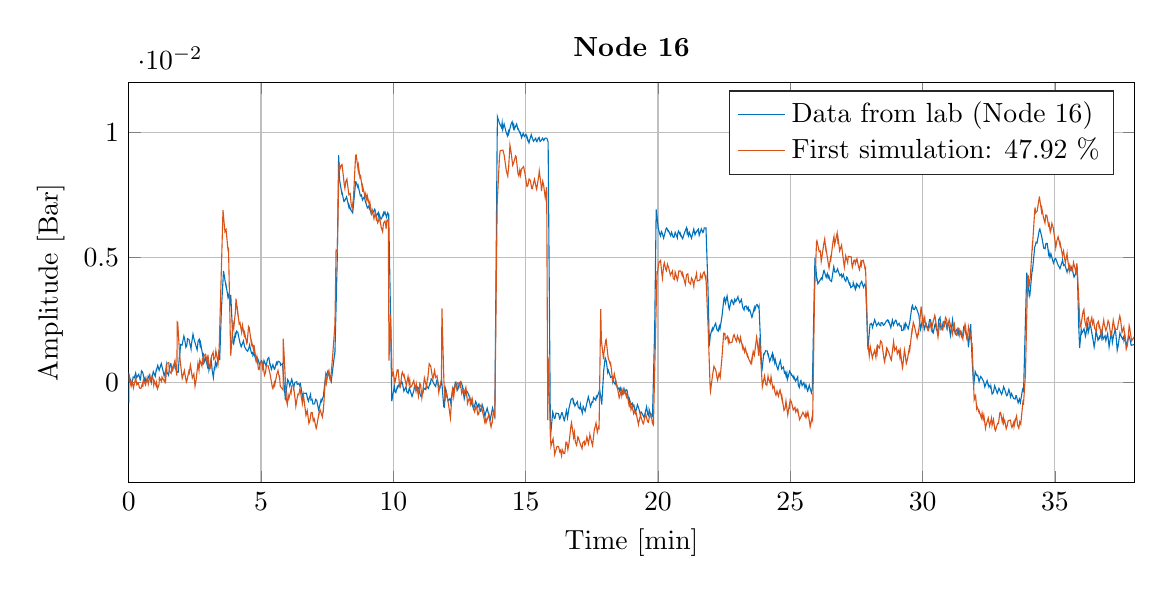
\begin{tikzpicture}

\begin{axis}[%
width=5.028in,
height=2in,
at={(1.011in,0.642in)},
scale only axis,
xmin=0,
xmax=38,
xlabel={Time [min]},
xmajorgrids,
ymin=-0.004,
ymax=0.012,
ylabel={Amplitude [Bar]},
ymajorgrids,
axis background/.style={fill=white},
title style={font=\bfseries},
title={Node 16},
legend style={legend cell align=left,align=left,draw=white!15!black}
]
\addplot [color=mycolor1,solid]
  table[row sep=crcr]{%
0.000833333333333333	-0.000818830449657984\\
0.01	0.000293887047898234\\
0.1175	-9.23886119253287e-05\\
0.169166666666667	0.000219937878788601\\
0.210833333333333	0.000186878250245617\\
0.2625	0.000377406109482642\\
0.264166666666667	0.000367836217009684\\
0.299166666666667	0.000196448142718311\\
0.3775	0.000322596725318952\\
0.438333333333333	9.4659286412252e-05\\
0.439166666666667	9.55292766370991e-05\\
0.483333333333333	0.000466145112413094\\
0.526666666666667	0.000411335728248516\\
0.6	8.59593841614631e-05\\
0.620833333333333	0.000161648533720929\\
0.650833333333333	7.00342130108278e-07\\
0.701666666666667	9.46592864151802e-05\\
0.776666666666667	0.000296497018571928\\
0.85	-6.25957966753077e-06\\
0.876666666666667	0.000227767790811531\\
0.883333333333333	0.000213847947213922\\
0.929166666666667	0.000433955474096637\\
1.0025	0.000246037585530212\\
1.04083333333333	0.000508774633428327\\
1.05166666666667	0.00049659477028112\\
1.09666666666667	0.000683642668622086\\
1.15083333333333	0.00049137482893262\\
1.22416666666667	0.000736712072337692\\
1.23083333333333	0.000758461827959814\\
1.315	0.000383496041056516\\
1.3375	0.000265177370478445\\
1.4025	0.00050007473118438\\
1.42166666666667	0.000679292717497448\\
1.44583333333333	0.000410465738022517\\
1.50416666666667	0.00029388704789679\\
1.56916666666667	0.000735842082110638\\
1.58833333333333	0.000749761925708414\\
1.64416666666667	0.000494854789829843\\
1.73	0.000783691544478812\\
1.7525	0.0005748938905175\\
1.76833333333333	0.000582723802542554\\
1.81333333333333	0.000423515591397861\\
1.86916666666667	0.00040698577712317\\
1.9275	0.00121868665688969\\
1.93583333333333	0.00117431715542442\\
1.95833333333333	0.0015223132453578\\
2.015	0.00149273357771525\\
2.08416666666667	0.00185986945259277\\
2.1125	0.00174242077223963\\
2.16166666666667	0.00140573455522568\\
2.19583333333333	0.00148316368523678\\
2.2225	0.00175460063538292\\
2.2775	0.00171806104594094\\
2.35583333333333	0.001337875317687\\
2.365	0.00148664364613293\\
2.42916666666667	0.0019312086510244\\
2.455	0.00178853025415546\\
2.54	0.00146837385141052\\
2.58583333333333	0.00130307570869914\\
2.62333333333333	0.00166151168132597\\
2.66666666666667	0.00172676094818454\\
2.69916666666667	0.00148577365591192\\
2.71583333333333	0.00158234257086928\\
2.7975	0.00107513826979937\\
2.81833333333333	0.00112211774193623\\
2.8475	0.000806311290324796\\
2.90416666666667	0.000979439345066571\\
2.97666666666667	0.000645363098723498\\
3.0025	0.000882870430102087\\
3.03083333333333	0.000490504838704844\\
3.11416666666667	0.000935069843604142\\
3.15333333333333	0.000495724780057966\\
3.2	0.000198188123164703\\
3.24	0.00064362311828145\\
3.2525	0.000492244819158966\\
3.27583333333333	0.000827191055720933\\
3.32833333333333	0.000640143157386711\\
3.40083333333333	0.00117605713587818\\
3.43833333333333	0.000898530254160729\\
3.50333333333333	0.00295170718474833\\
3.58333333333333	0.00446114022481266\\
3.59083333333333	0.00440372086997454\\
3.67416666666667	0.00386084696968721\\
3.68083333333333	0.00388607668620619\\
3.7525	0.00340062214076409\\
3.78	0.00350763093841419\\
3.835	0.00321009428153159\\
3.85666666666667	0.00350067101661904\\
3.94166666666667	0.00158234257086644\\
3.96666666666667	0.00153797306939833\\
4.02083333333333	0.00193468861192482\\
4.0375	0.00186334941348573\\
4.08	0.00205474726294778\\
4.12583333333333	0.00199384794721565\\
4.20416666666667	0.0015849525415423\\
4.2525	0.00142835430107521\\
4.335	0.00166586163244954\\
4.37916666666667	0.00142835430105888\\
4.44666666666667	0.0012995957477774\\
4.49416666666667	0.00124826632450988\\
4.54916666666667	0.00140747453566274\\
4.56583333333333	0.00149708352882283\\
4.64166666666667	0.00116735723360546\\
4.68166666666667	0.00120389682304745\\
4.6925	0.00108731813291496\\
4.72916666666667	0.0011708371944938\\
4.81666666666667	0.000865470625572975\\
4.82166666666667	0.000854160752647146\\
4.86583333333333	0.000979439345028199\\
4.90583333333333	0.00086982057670508\\
4.935	0.000726272189605873\\
5.0175	0.00086547062557725\\
5.07916666666667	0.000666242864091199\\
5.11166666666667	0.000879390469178926\\
5.19416666666667	0.000660152932531272\\
5.245	0.000934199853337647\\
5.295	0.000997709139761979\\
5.335	0.000725402199396222\\
5.34333333333333	0.000740192033223189\\
5.39	0.000522694476999111\\
5.44833333333333	0.000712352346008457\\
5.50166666666667	0.000526174437908769\\
5.51833333333333	0.000536614320612153\\
5.58166666666667	0.000794131427158049\\
5.60666666666667	0.000721052248262702\\
5.64666666666667	0.000850680791750283\\
5.71833333333333	0.00080892126096796\\
5.7375	0.000686252639269871\\
5.81083333333333	0.000755851857261236\\
5.8675	-8.86955034747061e-06\\
5.92166666666667	-0.000715301612902008\\
5.96333333333333	-0.000247246871955611\\
6.005	0.000114669061558853\\
6.04416666666667	4.50698435660729e-05\\
6.08583333333333	-0.000145458015660044\\
6.16166666666667	0.000132068866061666\\
6.2175	-0.000125448240488477\\
6.2275	-0.000227237096791164\\
6.28083333333333	-1.03963834408027e-06\\
6.35083333333333	3.28899804277333e-05\\
6.36416666666667	-7.32488269914039e-05\\
6.43083333333333	-4.80191104581945e-05\\
6.46166666666667	-0.00012805821114302\\
6.48916666666667	-6.10689638360223e-05\\
6.56833333333333	-0.000572623216029508\\
6.5725	-0.000622212658843643\\
6.605	-0.000434294770290541\\
6.72	-0.000429074828935991\\
6.74333333333333	-0.00058045312805706\\
6.74583333333333	-0.000570883235583214\\
6.78916666666667	-0.000747491251216162\\
6.8725	-0.00046822438905951\\
6.88833333333333	-0.000698771798631578\\
6.9275	-0.000669192130986179\\
6.96083333333333	-0.000862329960892402\\
7.02416666666667	-0.000852760068411437\\
7.0625	-0.00067615205278275\\
7.10583333333333	-0.000717911583587805\\
7.175	-0.00109809731181616\\
7.19	-0.00106329770282475\\
7.26833333333333	-0.000690941886611146\\
7.29083333333333	-0.00075358118279599\\
7.35583333333333	-0.000554353421315629\\
7.4425	0.00026952732157963\\
7.44583333333333	0.000235597702809232\\
7.52	0.000442655376314285\\
7.53166666666667	0.000393065933507269\\
7.61833333333333	0.000119019012683852\\
7.6525	2.85400293027482e-05\\
7.70583333333333	0.000496594770271877\\
7.79	0.00122303660799372\\
7.79333333333333	0.00121346671551988\\
7.88166666666667	0.00499183426196237\\
7.9325	0.0090920981915819\\
7.96916666666667	0.00809856935482327\\
8.05166666666667	0.00757570522971247\\
8.06166666666667	0.00759745498533317\\
8.13083333333333	0.00724597893451499\\
8.15666666666667	0.00725728880743515\\
8.23166666666667	0.00742432693060135\\
8.2325	0.00742606691105049\\
8.31916666666667	0.0070171715054077\\
8.3275	0.00709547062564053\\
8.3875	0.00691712262953144\\
8.46333333333333	0.00678488411536944\\
8.49416666666667	0.00710939046921948\\
8.57583333333333	0.00802636016616599\\
8.58333333333333	0.00803332008796827\\
8.65583333333333	0.00781843250243708\\
8.66916666666667	0.00787672184749692\\
8.75416666666667	0.0074652164711726\\
8.79583333333333	0.00749914608993589\\
8.8325	0.00729556837732059\\
8.9075	0.00743389682304819\\
8.93166666666667	0.00728077854345241\\
9.01916666666667	0.00698585185727763\\
9.07416666666667	0.00706415097747919\\
9.09166666666667	0.0069545322091447\\
9.10666666666667	0.0069780219452046\\
9.16333333333333	0.00675617443789389\\
9.19666666666667	0.0069014628054536\\
9.2175	0.00677966417397653\\
9.29083333333333	0.00692147258061238\\
9.35416666666667	0.00664742565979037\\
9.43	0.00679967394912108\\
9.45666666666667	0.0065708665199939\\
9.46833333333333	0.00671789486798713\\
9.5225	0.00655433670576468\\
9.55166666666667	0.00654302683282464\\
9.62666666666667	0.00677618421306687\\
9.635	0.00670919496577409\\
9.68166666666667	0.00682316368521226\\
9.7425	0.00661523602149469\\
9.7875	0.00678836407622367\\
9.825	0.0067161548875735\\
9.895	0.00262720083088408\\
9.94	-0.000746621260995145\\
10.0383333333333	-0.000151547947174493\\
10.065	-0.000379485386107659\\
10.0916666666667	-0.000408195063541991\\
10.15	-0.000171557722381574\\
10.1625	-0.000212447262944296\\
10.2166666666667	-7.41188172038998e-05\\
10.2516666666667	-0.000187217546445198\\
10.31	3.46299609195189e-05\\
10.3391666666667	-5.38958941508072e-06\\
10.3975	-0.000348165738031578\\
10.4775	-0.000174167693031843\\
10.5075	-0.000370785483840619\\
10.5608333333333	-0.000428204838689397\\
10.5941666666667	-0.000255946774185709\\
10.605	-0.000219407184738035\\
10.6833333333333	-0.00048040425219216\\
10.7066666666667	-0.000557833382211076\\
10.7708333333333	-0.000337725855322504\\
10.7941666666667	-0.000181997605050874\\
10.8775	-0.000305536217012611\\
10.9141666666667	-0.000186347556168753\\
10.9466666666667	-0.000216797214042289\\
11.0316666666667	-0.000538693597277581\\
11.0616666666667	-0.000576103176924955\\
11.0891666666667	-0.000369045503392895\\
11.1208333333333	-0.00040558509284909\\
11.145	-0.000222017155416726\\
11.2083333333333	-0.000281176490707538\\
11.2525	-0.000141108064471096\\
11.3233333333333	-0.000238546969645939\\
11.3833333333333	-3.49692570064813e-05\\
11.3983333333333	-4.80191103885697e-05\\
11.43	0.000148598680405995\\
11.4733333333333	8.59593842197359e-05\\
11.5566666666667	-0.000100218523916909\\
11.5983333333333	-0.000158507868990965\\
11.6391666666667	7.11695503558124e-05\\
11.6658333333333	0.000130328885652314\\
11.7208333333333	-0.00020983729226845\\
11.7475	-0.00026986661779875\\
11.8216666666667	6.94295699194686e-05\\
11.8258333333333	8.85693548700051e-05\\
11.905	-0.000969338758559563\\
11.9258333333333	-0.000985868572828563\\
11.97	-0.000239416959925229\\
11.9966666666667	-0.000329025953075365\\
12.065	-0.000723131524952292\\
12.1333333333333	-0.000652662316698693\\
12.1675	-0.000818830449648145\\
12.1716666666667	-0.000784030840659575\\
12.2483333333333	-0.000214187243428962\\
12.2891666666667	-0.000343815786916543\\
12.345	1.28802053130234e-05\\
12.3633333333333	2.15801075686972e-05\\
12.4108333333333	-0.000324676001943261\\
12.4383333333333	-0.000276826539603856\\
12.4941666666667	-2.01794232647795e-05\\
12.5533333333333	3.63699413558766e-05\\
12.6091666666667	-0.000131538172029932\\
12.6791666666667	-0.000650052346028537\\
12.7091666666667	-0.000504763978485867\\
12.7325	-0.000295096334306383\\
12.7983333333333	-0.000374265444767333\\
12.8716666666667	-0.000565663294227248\\
12.9575	-0.000841450195516874\\
12.9658333333333	-0.000804910606074891\\
13.0275	-0.00106155772241112\\
13.0508333333333	-0.00100500835778194\\
13.1116666666667	-0.00075793113392951\\
13.1416666666667	-0.000842320185773418\\
13.1908333333333	-0.000992828494716089\\
13.23	-0.000871029863204906\\
13.295	-0.00115116671557547\\
13.3141666666667	-0.00113724687197095\\
13.355	-0.000883209726316239\\
13.4025	-0.00103893797657366\\
13.46	-0.00135474442816662\\
13.485	-0.00123207580646426\\
13.5458333333333	-0.00102849809386174\\
13.5791666666667	-0.00118422634410212\\
13.6591666666667	-0.00144783338224345\\
13.665	-0.00146871314764173\\
13.7475	-0.00101805821116403\\
13.8308333333333	-0.00137475420337939\\
13.835	-0.0013434345552891\\
13.9225	0.00968456153468407\\
13.9333333333333	0.0106302409090891\\
14.0133333333333	0.0103579339686892\\
14.0875	0.0101978557673281\\
14.1116666666667	0.0103875136363147\\
14.1325	0.010121296627526\\
14.185	0.0103431441348623\\
14.2683333333333	0.00998731813292619\\
14.315	0.00986377952098717\\
14.3475	0.0100290776637199\\
14.36	0.00995860845552311\\
14.445	0.0103196543988137\\
14.4883333333333	0.0104240532257823\\
14.5325	0.0101935058162102\\
14.5516666666667	0.0102996446236436\\
14.5733333333333	0.0101369564516038\\
14.6591666666667	0.010337924193502\\
14.7041666666667	0.0101421763929299\\
14.7125	0.0101587062072103\\
14.7983333333333	0.00994729858259444\\
14.8041666666667	0.00996469838710294\\
14.845	0.00979244032260208\\
14.9058333333333	0.00996817834798987\\
14.9508333333333	0.00984115977518098\\
15.0091666666667	0.00992467883673424\\
15.0575	0.00975590073314589\\
15.0608333333333	0.00979766026393673\\
15.1258333333333	0.00958364266866493\\
15.1491666666667	0.00968282155426477\\
15.2116666666667	0.00991249897361723\\
15.2358333333333	0.00982636994135401\\
15.2958333333333	0.00964889193548157\\
15.38	0.00977330053763734\\
15.4075	0.0096497619257097\\
15.4241666666667	0.00963236212120688\\
15.4916666666667	0.00979418030302992\\
15.5075	0.00980723015639211\\
15.545	0.00964019203321169\\
15.5875	0.00967934159335794\\
15.6383333333333	0.00977330053765155\\
15.685	0.00968282155425908\\
15.7358333333333	0.00977765048873533\\
15.8016666666667	0.00976895058649671\\
15.8491666666667	0.00962366221895973\\
15.9366666666667	-0.00215513543500907\\
15.9383333333333	-0.00216731529816304\\
16.0233333333333	-0.00117117649076266\\
16.0241666666667	-0.00117378646143851\\
16.0816666666667	-0.00143739349955711\\
16.1116666666667	-0.00142434364617219\\
16.1458333333333	-0.00122424589445945\\
16.245	-0.00125034560121225\\
16.2833333333333	-0.00145392331379771\\
16.2891666666667	-0.00146349320626445\\
16.3641666666667	-0.00120858607040435\\
16.3791666666667	-0.00120945606064669\\
16.4608333333333	-0.00153396241450099\\
16.4616666666667	-0.00153309242427571\\
16.5416666666667	-0.00111984706744823\\
16.5816666666667	-0.00141042380255345\\
16.6366666666667	-0.00103284804497394\\
16.7175	-0.000671802101683341\\
16.7775	-0.000630912561083677\\
16.8	-0.000794470723368648\\
16.8125	-0.000753581182803095\\
16.8608333333333	-0.000937149120246825\\
16.9533333333333	-0.000765761045968413\\
16.9866666666667	-0.000986738563048165\\
17.0433333333333	-0.00105111783969636\\
17.0683333333333	-0.000896259579692638\\
17.075	-0.00096324882699679\\
17.1416666666667	-0.00121902595309638\\
17.1733333333333	-0.000959768866112709\\
17.2466666666667	-0.00114942673508796\\
17.2508333333333	-0.00112680698924482\\
17.3283333333333	-0.000755321163247974\\
17.3683333333333	-0.000571753225781499\\
17.425	-0.0008327502932612\\
17.4508333333333	-0.000961508846549067\\
17.5108333333333	-0.000774460948192821\\
17.5366666666667	-0.000789250781988535\\
17.5666666666667	-0.000602202883635133\\
17.6491666666667	-0.000710081671590104\\
17.6708333333333	-0.000552613440876426\\
17.695	-0.000600462903255619\\
17.775	-0.000364695552263636\\
17.795	-0.000281176490673427\\
17.8616666666667	-0.000753581182757618\\
17.875	-0.000878859775144347\\
17.95	0.000483544916901169\\
18.005	0.000980309335350107\\
18.0491666666667	0.000842850879812257\\
18.1008333333333	0.000403505816214927\\
18.125	0.000487024877842093\\
18.2116666666667	0.000206018035178029\\
18.2691666666667	0.000247777565980239\\
18.2916666666667	2.76700391087237e-05\\
18.3033333333333	8.76993645850394e-05\\
18.3825	-7.41188172607432e-05\\
18.405	6.8559579634489e-05\\
18.4758333333333	-0.000260296725329165\\
18.5175	-0.000221147165225546\\
18.55	-0.000331635923756887\\
18.5758333333333	-0.000219407184780668\\
18.6375	-0.000443864662767232\\
18.6608333333333	-0.000472574340127666\\
18.7191666666667	-0.000259426735103888\\
18.7433333333333	-0.000396015200365293\\
18.7975	-0.000288136412566642\\
18.8258333333333	-0.000295096334380282\\
18.9083333333333	-0.000776200928597912\\
18.9216666666667	-0.000663102199379359\\
18.985	-0.000886689687061057\\
19.0375	-0.00083101031269979\\
19.0541666666667	-0.000966728787787072\\
19.09	-0.000908439442681749\\
19.1458333333333	-0.00119031627554836\\
19.1758333333333	-0.00109983729215304\\
19.2241666666667	-0.000888429667522991\\
19.27	-0.00101718822083074\\
19.3241666666667	-0.00125295557173462\\
19.3733333333333	-0.00118944628533445\\
19.4383333333333	-0.00132081480937489\\
19.4758333333333	-0.00140259389053443\\
19.5258333333333	-0.00116421656884672\\
19.57	-0.000975428689994437\\
19.6116666666667	-0.00127731529798569\\
19.6525	-0.00133995459418333\\
19.6658333333333	-0.00108417746808658\\
19.7025	-0.00121206603120316\\
19.7483333333333	-0.00141651373401959\\
19.7933333333333	-0.00133821461376686\\
19.8766666666667	0.00219742565996381\\
19.9325	0.00691973260020728\\
20.0116666666667	0.00617241099696213\\
20.0516666666667	0.00599232302047067\\
20.0941666666667	0.00586704442818342\\
20.1308333333333	0.00604278245348593\\
20.1458333333333	0.0060192927174374\\
20.2141666666667	0.00577395547411226\\
20.2291666666667	0.00584007473113712\\
20.305	0.0061471812804403\\
20.33	0.00618111089921496\\
20.385	0.00604539242420725\\
20.4016666666667	0.00606888216028989\\
20.4791666666667	0.00587313435973766\\
20.515	0.006008852834734\\
20.5691666666667	0.00582180493644598\\
20.6025	0.00580440513196305\\
20.6508333333333	0.00600363289345052\\
20.7341666666667	0.00578178538616254\\
20.75	0.00598275312803236\\
20.7775	0.00605409232643735\\
20.8391666666667	0.00590967394912564\\
20.8458333333333	0.00596361334306476\\
20.9166666666667	0.00577656544481084\\
20.9316666666667	0.00575046573802962\\
21.015	0.00602886260995529\\
21.0775	0.00618807082100585\\
21.1	0.00598710307917014\\
21.1175	0.00606975215053791\\
21.1558333333333	0.00586965439885927\\
21.1908333333333	0.00599754296184511\\
21.2675	0.00576960552300858\\
21.2775	0.0058096250733318\\
21.3525	0.00613761138804177\\
21.3991666666667	0.00590880395892879\\
21.4491666666667	0.00603843250240499\\
21.4591666666667	0.0060271226295161\\
21.5233333333333	0.00613500141736591\\
21.5575	0.00588879418379275\\
21.6266666666667	0.00611151168126053\\
21.6366666666667	0.00614631129023775\\
21.6975	0.00599841295207039\\
21.7183333333333	0.00602451265881183\\
21.7483333333333	0.00618546085036979\\
21.8141666666667	0.00618111089928317\\
21.89	0.00378080786897823\\
21.94	0.00145967394912856\\
21.9775	0.0018937990712264\\
22.055	0.00216436603118705\\
22.0733333333333	0.00208954687186957\\
22.1525	0.00230878440851012\\
22.18	0.00236794374380093\\
22.2316666666667	0.00210520669593035\\
22.2741666666667	0.00205561725307786\\
22.3175	0.00225397502423204\\
22.3425	0.0021426162754072\\
22.4158333333333	0.00262807082108663\\
22.495	0.00336843250254656\\
22.5166666666667	0.00339975215070222\\
22.55	0.00317877463362816\\
22.6116666666667	0.00345804149577345\\
22.6783333333333	0.00299172673518097\\
22.695	0.00293082741942254\\
22.7658333333333	0.00327708352900555\\
22.7891666666667	0.00331101314775747\\
22.8475	0.00313788509300576\\
22.8608333333333	0.00312309525916458\\
22.9008333333333	0.0033258029816555\\
22.9408333333333	0.0032405439396062\\
23.0208333333333	0.00342759183788854\\
23.0283333333333	0.00337104247325652\\
23.0916666666667	0.0031926944770849\\
23.1533333333333	0.00331797306957111\\
23.2016666666667	0.00300999652995738\\
23.2533333333333	0.00290211774202231\\
23.2808333333333	0.00304392614873206\\
23.3375	0.00305871598255049\\
23.3658333333333	0.00293778734124754\\
23.4091666666667	0.00301086652017131\\
23.4216666666667	0.00286383817212123\\
23.4658333333333	0.00291168763450042\\
23.5508333333333	0.00260197111433381\\
23.5533333333333	0.00260545107523495\\
23.6416666666667	0.00300303660813239\\
23.6608333333333	0.00290472771268679\\
23.7175	0.00309699555242883\\
23.7441666666667	0.00311874530807228\\
23.8083333333333	0.00296910698935204\\
23.8191666666667	0.0030239163735335\\
23.9041666666667	0.000893310312878662\\
23.9283333333333	0.00046005518094358\\
23.9891666666667	0.00108122820152841\\
23.9916666666667	0.00107426827974319\\
24.0691666666667	0.00126827609978232\\
24.1266666666667	0.00126044618777751\\
24.1566666666667	0.00110993787888315\\
24.1675	0.00112559770294962\\
24.2225	0.000845460850556326\\
24.3233333333333	0.00116039731185293\\
24.3416666666667	0.000945509726338792\\
24.3641666666667	0.00104729858267416\\
24.4116666666667	0.000783691544572598\\
24.4333333333333	0.000908970136979229\\
24.4808333333333	0.000680162707763943\\
24.5341666666667	0.000513994574746282\\
24.57	0.000692342570878107\\
24.6233333333333	0.000869820576818767\\
24.675	0.000540964271821001\\
24.7408333333333	0.000619263392016872\\
24.7791666666667	0.000385236021483992\\
24.8058333333333	0.000423515591362333\\
24.84	0.000258217448581316\\
24.8691666666667	0.000385236021438515\\
24.89	0.000119889002875032\\
24.9741666666667	0.000453965249247235\\
25.0408333333333	0.000307806891467921\\
25.0466666666667	0.00032346671552301\\
25.13	0.000161648533722705\\
25.1391666666667	0.000236467693051565\\
25.2025	5.55097262609355e-05\\
25.28	0.000227767790776004\\
25.3033333333333	-0.000106308455499568\\
25.34	-0.000197657429171327\\
25.3875	6.07296675785296e-05\\
25.4025	8.07394427429775e-05\\
25.4458333333333	-0.000123708260045027\\
25.5108333333333	-4.51959924947787e-06\\
25.555	-0.000218537194566756\\
25.5908333333333	-8.28187194567287e-05\\
25.6533333333333	-0.000351645698898603\\
25.6591666666667	-0.000346425757569643\\
25.7166666666667	-0.000109788416440493\\
25.7425	-0.000214187243377809\\
25.7991666666667	-0.000408195063519259\\
25.8308333333333	-0.000242896920868985\\
25.9175	0.00427148235582746\\
25.9325	0.0049796543988553\\
26.005	0.00411401412514789\\
26.0158333333333	0.00412706397849871\\
26.0416666666667	0.0039469760019902\\
26.0983333333333	0.00404354491691135\\
26.1725	0.00418274335291113\\
26.2025	0.00412793396874674\\
26.2608333333333	0.00446462018569815\\
26.2758333333333	0.00448201999020949\\
26.3558333333333	0.00420971304991764\\
26.4	0.00435239144673898\\
26.4291666666667	0.00418361334311368\\
26.4575	0.00426800239487517\\
26.5025	0.00408965439883997\\
26.5591666666667	0.00404093494624687\\
26.6166666666667	0.00445331031281494\\
26.6425	0.00463078831867034\\
26.685	0.00441590073309368\\
26.7325	0.00441764071355562\\
26.7883333333333	0.00454117932550031\\
26.7933333333333	0.00450724970671997\\
26.8758333333333	0.00427235234605843\\
26.9266666666667	0.0043367316226043\\
26.9533333333333	0.00420101314752838\\
27.005	0.00432281177902251\\
27.0516666666667	0.00411749408602628\\
27.0975	0.00404963484856791\\
27.1325	0.00421580298142073\\
27.1533333333333	0.0041949232159912\\
27.2308333333333	0.00393392614861096\\
27.25	0.00396872575759954\\
27.285	0.00379646769312426\\
27.3633333333333	0.00385910698927074\\
27.3783333333333	0.003998305425208\\
27.4575	0.00372773846536671\\
27.4925	0.00392522624639224\\
27.5116666666667	0.00384518714578559\\
27.5325	0.00392783621711924\\
27.6141666666667	0.00380516759532025\\
27.6441666666667	0.00394436603131436\\
27.7	0.00404354491689997\\
27.7566666666667	0.00383648724345886\\
27.765	0.00380603758559102\\
27.8125	0.00392957619744476\\
27.8483333333333	0.00388868665684509\\
27.9316666666667	0.00135440513192617\\
27.9341666666667	0.00134831520034918\\
28.0125	0.00232792419338108\\
28.0666666666667	0.00236098382194183\\
28.1066666666667	0.00221656544461309\\
28.1075	0.0022104755130361\\
28.19	0.00251410210155752\\
28.1941666666667	0.00250192223840355\\
28.26	0.00227398479950448\\
28.3383333333333	0.00239752341143214\\
28.365	0.00231139437915755\\
28.4175	0.00226876485810731\\
28.43	0.00239056348959008\\
28.4833333333333	0.00238621353846366\\
28.5166666666667	0.00228616466260161\\
28.545	0.00230878440845896\\
28.6283333333333	0.00245755273694823\\
28.6825	0.00250627218952996\\
28.7016666666667	0.00242449310837611\\
28.7191666666667	0.00245233279558517\\
28.7983333333333	0.00219307570858729\\
28.8066666666667	0.00223918519051022\\
28.8575	0.00249496231661266\\
28.8975	0.00230008450619476\\
28.9725	0.00249061236550897\\
28.9916666666667	0.00249148235574563\\
29.055	0.00228355469199397\\
29.11	0.002366203763339\\
29.1575	0.00224962507316247\\
29.1875	0.00226354491673288\\
29.2083333333333	0.00208171695977381\\
29.2775	0.00210433670571075\\
29.3025	0.00230965439876382\\
29.3325	0.00218089584545038\\
29.3608333333333	0.00236533377310234\\
29.455	0.00214348626571205\\
29.5066666666667	0.00238969349938753\\
29.5108333333333	0.00238534354827248\\
29.595	0.00303087629536418\\
29.6191666666667	0.00308394569910643\\
29.6508333333333	0.00292908743901744\\
29.6925	0.00291777756599783\\
29.7333333333333	0.00303522624641102\\
29.775	0.00294996720440151\\
29.8575	0.00269332008795442\\
29.925	0.00213304638315645\\
29.945	0.00222787531769524\\
30.0091666666667	0.00261676094815226\\
30.0325	0.00239056348966966\\
30.0608333333333	0.00211390659816613\\
30.13	0.00236533377314782\\
30.1925	0.00213826632439447\\
30.2133333333333	0.0021808958454788\\
30.2633333333333	0.00251845205274077\\
30.3008333333333	0.0025062721895186\\
30.375	0.00201820767338501\\
30.4025	0.00198079809377742\\
30.4683333333333	0.00232792419348339\\
30.4866666666667	0.00235315390997112\\
30.5233333333333	0.00211303660795222\\
30.575	0.00204169740955291\\
30.61	0.00251323211145728\\
30.6591666666667	0.0026028411045932\\
30.6925	0.00214000630495871\\
30.7516666666667	0.00223135527853384\\
30.775	0.00242188313775711\\
30.8641666666667	0.00243319301064031\\
30.9083333333333	0.0022504950634389\\
30.9175	0.00217480591385634\\
30.98	0.00238273357766484\\
30.9958333333333	0.00228964462364485\\
31.0508333333333	0.00188335918856848\\
31.1325	0.00250627218956408\\
31.165	0.00218002585519668\\
31.1741666666667	0.00223657521982869\\
31.2258333333333	0.00199471793738194\\
31.3075	0.00214348626578027\\
31.3266666666667	0.00198340806442485\\
31.3491666666667	0.00209389682297893\\
31.3716666666667	0.00189553905172243\\
31.4558333333333	0.00202255762460236\\
31.4816666666667	0.00183985967731001\\
31.5216666666667	0.00194947844563882\\
31.5533333333333	0.00220960552285629\\
31.6091666666667	0.00209389682298462\\
31.67	0.00178940024432318\\
31.7008333333333	0.0018868391494696\\
31.7325	0.00140225459432809\\
31.8166666666667	0.00233488411526292\\
31.8716666666667	0.000888960361678362\\
31.9291666666667	-0.000135888123153502\\
31.9866666666667	0.000437435435012332\\
32.0458333333333	0.000274747262884428\\
32.0825	0.000293017057626743\\
32.1333333333333	3.63699413331309e-05\\
32.1341666666667	3.9849902234268e-05\\
32.195	0.000240817644155247\\
32.2258333333333	0.000203408064479452\\
32.3091666666667	2.59300584990046e-05\\
32.3508333333333	-0.000176777663844122\\
32.4375	7.55195014253834e-05\\
32.4816666666667	-0.000115008357803564\\
32.4858333333333	-7.41188172152657e-05\\
32.5716666666667	-0.000220277174977523\\
32.58	-0.000151547947225647\\
32.6258333333333	-0.000464744428100114\\
32.6741666666667	-0.000400365151497398\\
32.7225	-0.000132408162309222\\
32.7491666666667	-0.000212447262978407\\
32.8208333333333	-0.000436034750705569\\
32.8375	-0.000394275219960202\\
32.8841666666667	-0.000233327028356767\\
32.925	-0.00032641598238814\\
32.9841666666667	-0.00047518431078078\\
33.0183333333333	-0.000380355376264727\\
33.0616666666667	-0.00016981774193385\\
33.11	-0.000307276197500136\\
33.1725	-0.00052651373405542\\
33.2041666666667	-0.000504763978434714\\
33.2591666666667	-0.000279436510302447\\
33.2891666666667	-0.000378615395916479\\
33.3208333333333	-0.000576103176896534\\
33.3608333333333	-0.000446474633420332\\
33.4425	-0.000645702394856645\\
33.4983333333333	-0.000659622238410013\\
33.5266666666667	-0.000529993694967909\\
33.5391666666667	-0.000529993694967909\\
33.6116666666667	-0.000811870527754929\\
33.6575	-0.000661362218889003\\
33.695	-0.000804040615750123\\
33.7116666666667	-0.000693551857230149\\
33.7783333333333	-0.000270736608060984\\
33.8158333333333	-0.000340335826026772\\
33.885	0.00242449310852959\\
33.9358333333333	0.00439676094827388\\
34.0316666666667	0.00347196133933249\\
34.055	0.00359375997076979\\
34.06	0.00357114022495221\\
34.1433333333333	0.00455161920815254\\
34.1558333333333	0.00452290953071252\\
34.2358333333333	0.00540507961884241\\
34.2908333333333	0.00561213729232332\\
34.3233333333333	0.00558342761494583\\
34.4108333333333	0.00609933181814068\\
34.4308333333333	0.00614022135866077\\
34.4983333333333	0.0058505146139201\\
34.5791666666667	0.0053720199902703\\
34.6283333333333	0.0053502702346496\\
34.66	0.00556341783982117\\
34.7108333333333	0.00555645791804164\\
34.7608333333333	0.0051371226295235\\
34.775	0.00520498186710694\\
34.8133333333333	0.00500053416424504\\
34.8483333333333	0.00514669252209256\\
34.9358333333333	0.00480739633428907\\
34.9425	0.00477694667641555\\
35.0058333333333	0.0049552946725758\\
35.0266666666667	0.00496399457478315\\
35.1108333333333	0.00471778734106221\\
35.1916666666667	0.0045542291787886\\
35.1983333333333	0.00458293885622293\\
35.2858333333333	0.0048769955522435\\
35.29	0.0049074452101284\\
35.3258333333333	0.00468124775166853\\
35.3733333333333	0.00471865733140117\\
35.4575	0.00441764071347603\\
35.4616666666667	0.00444287043000924\\
35.525	0.00460642859232831\\
35.56	0.00445766026380494\\
35.6366666666667	0.00460816857272203\\
35.6383333333333	0.00461512849452429\\
35.7216666666667	0.00421493299113292\\
35.7358333333333	0.00423146280537919\\
35.8116666666667	0.00444983035182855\\
35.8441666666667	0.00453943934497016\\
35.8991666666667	0.00225832497555171\\
35.9341666666667	0.0013805048387074\\
35.9933333333333	0.00211999652984542\\
36.0125	0.00196078831877212\\
36.0991666666667	0.00214870620734228\\
36.1533333333333	0.00185116955031828\\
36.1616666666667	0.00189118910066992\\
36.2375	0.00234097404706728\\
36.2566666666667	0.0019955879276925\\
36.3366666666667	0.0023479339688468\\
36.3383333333333	0.0023522839199789\\
36.4183333333333	0.00181984990229904\\
36.4241666666667	0.00183202976540753\\
36.4825	0.00141878440854026\\
36.5166666666667	0.00164498186702286\\
36.5533333333333	0.00208171695997846\\
36.6266666666667	0.00169370131961596\\
36.6841666666667	0.00183202976545301\\
36.6975	0.00178157033232974\\
36.775	0.00207475703823302\\
36.7791666666667	0.002093896823212\\
36.815	0.00172937091890372\\
36.8941666666667	0.0018703093353086\\
36.9258333333333	0.00167543152486797\\
36.9925	0.00195904833832157\\
37.0375	0.00151883328445347\\
37.0466666666667	0.00142139437927864\\
37.125	0.00199210796674588\\
37.1308333333333	0.00207475703811934\\
37.1708333333333	0.0016032223363457\\
37.2133333333333	0.0018572594820601\\
37.2783333333333	0.0021130366081\\
37.3025	0.00195991832845022\\
37.3541666666667	0.00129437580642144\\
37.3875	0.00146228391988398\\
37.4558333333333	0.00197905811349738\\
37.475	0.00190771891499009\\
37.5558333333333	0.0017415507819781\\
37.6008333333333	0.00183637971648277\\
37.6108333333333	0.00166238167152852\\
37.6516666666667	0.00178853025415475\\
37.7075	0.00147011383183764\\
37.7375	0.00159539242431248\\
37.7933333333333	0.00189292908115458\\
37.8366666666667	0.00173198088955115\\
37.8808333333333	0.00148577365590409\\
38	0.0015205732648131\\
};
\addlegendentry{Data from lab (Node 16)};

\addplot [color=mycolor2,solid]
  table[row sep=crcr]{%
0.000833333333333333	3.07781400041399e-05\\
0.0175	0.000256691584528162\\
0.0891666666666667	-0.000146507257931168\\
0.125833333333333	4.70316487393499e-05\\
0.175	-0.000181690363611822\\
0.178333333333333	-0.000213440904247347\\
0.264166666666667	0.000181697443749201\\
0.306666666666667	-9.27308319101511e-05\\
0.3625	-2.45085221941198e-05\\
0.410833333333333	-0.00022662208337257\\
0.463333333333333	-0.000232680286295418\\
0.523333333333333	-2.26148841104195e-05\\
0.533333333333333	-0.000176339892696044\\
0.558333333333333	0.000103156416843841\\
0.634166666666667	-9.61706439201929e-05\\
0.695833333333333	0.000187540008962417\\
0.701666666666667	0.000149138780799371\\
0.74	-6.5249001321585e-05\\
0.8025	0.000270908756620918\\
0.8325	8.78585528871316e-05\\
0.908333333333333	0.000202424384118884\\
0.945	-0.000103131594096308\\
0.965833333333333	6.58755854355378e-05\\
1.03833333333333	-0.00013226346410377\\
1.05333333333333	-1.48820197005601e-05\\
1.0875	-0.000249717587323112\\
1.14583333333333	-7.14927011819157e-05\\
1.1575	0.000197022356854688\\
1.23833333333333	4.29431995164657e-05\\
1.25666666666667	0.000215524124281703\\
1.36416666666667	1.61238725347286e-05\\
1.3875	0.000283306943108313\\
1.4025	0.00016017346057594\\
1.44666666666667	0.000765652745711191\\
1.51333333333333	0.000792212717534111\\
1.535	0.000454083520427996\\
1.60166666666667	0.000364101481589142\\
1.63333333333333	0.000636593780835671\\
1.66666666666667	0.000504700709050712\\
1.74833333333333	0.000878310506742091\\
1.81833333333333	0.000274322380117102\\
1.83583333333333	0.00241617680606232\\
1.8525	0.00239059116187559\\
1.9275	0.00105253899149711\\
2.0125	0.000231301722405356\\
2.02166666666667	0.000163850286226788\\
2.10166666666667	0.000475110275641116\\
2.1025	0.000465715913306407\\
2.1775	1.45422507850097e-05\\
2.19833333333333	6.52438829772425e-05\\
2.2725	0.00044719766811767\\
2.28833333333333	0.000390613155436441\\
2.33083333333333	0.000699807624635542\\
2.36583333333333	0.000475314043251667\\
2.40416666666667	0.000180655314397622\\
2.46166666666667	0.000338662381617341\\
2.50583333333333	-0.000149384185718703\\
2.54416666666667	8.18307875700276e-05\\
2.61583333333333	0.000764858918668778\\
2.65583333333333	0.000482922771540744\\
2.68666666666667	0.000897637040171275\\
2.76666666666667	0.000656880954612473\\
2.7925	0.00100600949015722\\
2.82166666666667	0.000718396002540811\\
2.85	0.00108955256140665\\
2.90416666666667	0.00112906774127911\\
2.96916666666667	0.000822178326058739\\
2.995	0.00111159653291741\\
3.03416666666667	0.000651499216195795\\
3.07916666666667	0.000577809044731559\\
3.12666666666667	0.00104948050439517\\
3.19	0.0012100603361985\\
3.20916666666667	0.000924799256171951\\
3.2625	0.000986315201632886\\
3.29333333333333	0.00127547819463815\\
3.37666666666667	0.000764855724536145\\
3.415	0.00131289831185782\\
3.41666666666667	0.00129738328276606\\
3.50333333333333	0.00460048561885768\\
3.5625	0.00689720209481069\\
3.60166666666667	0.00642923584521238\\
3.63666666666667	0.00603074195020459\\
3.67916666666667	0.00611606508194301\\
3.76	0.00521440559271807\\
3.77083333333333	0.00539147307071246\\
3.85333333333333	0.00111081818103303\\
3.85666666666667	0.00107907383872924\\
3.94	0.0023662738565656\\
3.97083333333333	0.00218551104088638\\
4.02916666666667	0.00281527968970162\\
4.055	0.0033489680940842\\
4.11416666666667	0.00281467514711486\\
4.11833333333333	0.0028545305006788\\
4.17416666666667	0.00234423008666477\\
4.20416666666667	0.00239691580979391\\
4.2675	0.00200665341908673\\
4.29916666666667	0.00228634069456465\\
4.36333333333333	0.00188737892313173\\
4.37916666666667	0.00199355801943405\\
4.4625	0.00155931498184001\\
4.47666666666667	0.00159878458780849\\
4.52833333333333	0.00223839385243582\\
4.55416666666667	0.0021938350221306\\
4.63333333333333	0.00157828341281538\\
4.64166666666667	0.00164536168054911\\
4.72166666666667	0.001293172233634\\
4.73333333333333	0.0015003976065612\\
4.81666666666667	0.000858014287102757\\
4.84416666666667	0.00102424351350068\\
4.90166666666667	0.000530974341368513\\
4.92666666666667	0.000512873530874854\\
4.97166666666667	0.000769760437405194\\
5.03916666666667	0.000829001700143473\\
5.055	0.000563506118858844\\
5.08083333333333	0.000683657527656734\\
5.13083333333333	0.000291492533930679\\
5.17083333333333	0.00039503403648593\\
5.19666666666667	0.000659326517119956\\
5.26916666666667	0.000667099879853056\\
5.3425	0.000334727578231478\\
5.43	-0.000206252350373117\\
5.4475	-0.000248746871096431\\
5.50166666666667	-1.16320855508083e-05\\
5.5175	-0.000109518146382904\\
5.59916666666667	0.000341572653553459\\
5.64166666666667	0.000477461748690368\\
5.6925	0.000194242816414536\\
5.6975	0.000284767977808143\\
5.7275	-0.000149722048119607\\
5.83333333333333	-0.000296390871291197\\
5.83583333333333	0.00175272296183345\\
5.8675	0.00121515552146315\\
5.955	-0.000689182234647684\\
5.99166666666667	-0.000879360771394085\\
6.02333333333333	-0.000499612722017293\\
6.05166666666667	-0.000642627374241826\\
6.12916666666667	-0.000306570296795731\\
6.14083333333333	-0.000368297034623457\\
6.15666666666667	-0.000138290960094817\\
6.22416666666667	-0.000112703888240571\\
6.305	-0.000810206364497569\\
6.31583333333333	-0.00094488422282269\\
6.3925	-0.000465655337445907\\
6.42833333333333	-0.000487116669403394\\
6.47166666666667	-0.000236115462841123\\
6.48083333333333	-0.000309002040694889\\
6.5625	-0.000849082917442003\\
6.6025	-0.000501379437946079\\
6.65583333333333	-0.000962152540105566\\
6.65666666666667	-0.000961129966464487\\
6.69833333333333	-0.00131528321547872\\
6.74666666666667	-0.00111835645240561\\
6.80916666666667	-0.00163276356143139\\
6.85166666666667	-0.00150474960273228\\
6.8925	-0.00119791451193142\\
6.93416666666667	-0.00120289712548952\\
6.9725	-0.00153163105920822\\
7.00666666666667	-0.00144926913678806\\
7.085	-0.00184285059216315\\
7.095	-0.00181265552738151\\
7.18	-0.00127965378321874\\
7.1825	-0.00131153619072339\\
7.22916666666667	-0.0010828502169249\\
7.3175	-0.00137909662257568\\
7.355	-0.00105260789672195\\
7.35916666666667	-0.00106946565705702\\
7.4425	0.000309724315663927\\
7.47416666666667	-9.19360723747437e-06\\
7.53083333333333	0.000369828076602408\\
7.565	0.000479037924940818\\
7.61583333333333	9.19599864886886e-05\\
7.63083333333333	9.11447749932351e-05\\
7.70583333333333	0.00105199658139314\\
7.79333333333333	0.00232809944760671\\
7.83583333333333	0.00529420271231424\\
7.88166666666667	0.00524100745511059\\
7.95166666666667	0.00882046622153414\\
7.9775	0.00852420084053243\\
8.035	0.00870180857788167\\
8.0625	0.00871895807611993\\
8.14416666666667	0.00792405025106521\\
8.16916666666667	0.00776731582304753\\
8.20333333333333	0.00803693476551111\\
8.245	0.00813898588247667\\
8.31916666666667	0.00751307041444584\\
8.36833333333333	0.00756211806279914\\
8.40666666666667	0.00713406475739565\\
8.445	0.00696958294986611\\
8.49333333333333	0.00739854996328551\\
8.49416666666667	0.00739798008591418\\
8.57333333333333	0.00908614154882355\\
8.595	0.00910194334975208\\
8.66916666666667	0.00850583857380564\\
8.6825	0.00866709288370981\\
8.74666666666667	0.00812561188902565\\
8.7575	0.00830835030026308\\
8.8425	0.00763061686360937\\
8.8475	0.00781531781501712\\
8.93083333333333	0.00743153145045295\\
8.95666666666667	0.00755343997901503\\
8.99916666666667	0.00729049189929849\\
9.01916666666667	0.00745501093507163\\
9.095	0.00709031194681666\\
9.115	0.00720480923393702\\
9.17166666666667	0.00675094419990029\\
9.21	0.00686585400768193\\
9.26833333333333	0.00655355528167781\\
9.32333333333333	0.00682383180438666\\
9.355	0.00654433188576409\\
9.3725	0.00660368193476665\\
9.4075	0.00639045005432825\\
9.48416666666667	0.00658146700780529\\
9.54416666666667	0.00619418534870829\\
9.595	0.00602792449071312\\
9.62666666666667	0.00637216202099085\\
9.68333333333333	0.00645745496882096\\
9.72	0.00622980414429094\\
9.72583333333333	0.00614713712645422\\
9.75666666666667	0.00649353655484238\\
9.80916666666667	0.00651177562984108\\
9.83583333333333	0.000870984303739517\\
9.895	0.0027134246802651\\
9.955	0.000260015229213286\\
10	0.000392406930041023\\
10.0575	-5.18456070193116e-06\\
10.0833333333333	0.000108769516987571\\
10.1458333333333	0.000506436658540157\\
10.1808333333333	0.000508094476301371\\
10.2291666666667	-7.13257278582907e-05\\
10.2633333333333	-0.000145317636642048\\
10.3233333333333	0.000348496317598225\\
10.34	0.000413342674908458\\
10.4183333333333	0.000190612084030134\\
10.4208333333333	0.000223932850162047\\
10.4891666666667	-0.000122426137139651\\
10.5558333333333	0.000242455320293071\\
10.5916666666667	-3.42599676940603e-05\\
10.6191666666667	0.000101493575658723\\
10.6408333333333	-0.000192653871576025\\
10.6841666666667	-0.000159937980445169\\
10.77	6.93008863873789e-05\\
10.7708333333333	5.67222120371304e-05\\
10.8516666666667	-0.000334279689040668\\
10.8691666666667	-6.84374933974689e-05\\
10.9416666666667	-0.000497067100341645\\
10.9491666666667	-0.000548378772566426\\
11.0016666666667	-3.15631896336786e-05\\
11.0333333333333	-8.94634959276255e-05\\
11.0766666666667	-0.000615461539568615\\
11.1208333333333	-0.00028909726133161\\
11.1725	0.000185513988876918\\
11.2558333333333	-0.000185660463888711\\
11.29	0.00019701701205724\\
11.2958333333333	8.95514986874396e-05\\
11.355	0.000748127997994173\\
11.4125	0.000652005278033072\\
11.4691666666667	0.000267303459640103\\
11.4975	0.000148483715743488\\
11.5583333333333	0.000477409511531121\\
11.5966666666667	0.000205496134086203\\
11.6508333333333	0.000268037775285635\\
11.7175	-0.000402358194231829\\
11.7358333333333	-0.000271549620215424\\
11.8183333333333	0.000138573358862159\\
11.8358333333333	0.00296446996102659\\
11.9091666666667	9.42110430079839e-05\\
11.9533333333333	-0.000692787469186632\\
12.0033333333333	-0.00042601679192179\\
12.0841666666667	-0.000858882764239025\\
12.1558333333333	-0.00142207721279306\\
12.1716666666667	-0.00118065551372189\\
12.2391666666667	-0.000201643157578543\\
12.2816666666667	-0.000571096642048986\\
12.3375	-7.60262686411104e-05\\
12.4016666666667	-0.000234486202456053\\
12.4158333333333	-1.62645572182872e-05\\
12.4875	-2.13524963667745e-05\\
12.5133333333333	-0.000151574413729774\\
12.5383333333333	-4.25004527616405e-05\\
12.585	-0.000446008022130808\\
12.6483333333333	-0.000276311836618983\\
12.6791666666667	-0.000437757475381257\\
12.74	-0.000194431181913848\\
12.7825	-0.000612508932550642\\
12.785	-0.000564504706991599\\
12.8	-0.000848591358728418\\
12.885	-0.00057289489093144\\
12.9108333333333	-0.000879199002539848\\
12.9766666666667	-0.000628641029662373\\
13.0458333333333	-0.00110088835459516\\
13.0716666666667	-0.00117540049299106\\
13.1225	-0.000944854609943584\\
13.1516666666667	-0.00103209085970698\\
13.1958333333333	-0.00129306291171874\\
13.2316666666667	-0.00125758382389614\\
13.2633333333333	-0.00088902340781977\\
13.33	-0.000969925757872312\\
13.3975	-0.00129667217724205\\
13.3991666666667	-0.00127092331481592\\
13.455	-0.00158528729240154\\
13.4916666666667	-0.00144586787922239\\
13.5058333333333	-0.00160131624427815\\
13.6091666666667	-0.00128327713794172\\
13.6416666666667	-0.00150865000703075\\
13.6916666666667	-0.00178086133260054\\
13.7466666666667	-0.00148509215024823\\
13.7475	-0.00148934883188948\\
13.7766666666667	-0.00116925070338975\\
13.835	-0.00134917130753207\\
13.9225	0.00708092378637431\\
14.0091666666667	0.00901228440095978\\
14.01	0.00900438597342053\\
14.035	0.00926772664475469\\
14.1408333333333	0.0092975343821677\\
14.185	0.00911250714826882\\
14.2716666666667	0.00845250460701235\\
14.3241666666667	0.00825466119685034\\
14.3591666666667	0.00867605410031104\\
14.3616666666667	0.00866898733084096\\
14.4058333333333	0.0094926491695949\\
14.4516666666667	0.00919384379214874\\
14.51	0.00868544626579973\\
14.5358333333333	0.00874718407130634\\
14.62	0.00906355505935468\\
14.6391666666667	0.00903437532735335\\
14.7108333333333	0.0083569068363979\\
14.7425	0.00825877912251349\\
14.7775	0.00848638686619603\\
14.8083333333333	0.00829418869833748\\
14.8383333333333	0.00852925958691547\\
14.9208333333333	0.00863683085683786\\
14.9733333333333	0.00836219228400731\\
15.0483333333333	0.00784444513809142\\
15.0825	0.00786880848245663\\
15.1275	0.00814034798262838\\
15.1783333333333	0.00807927154223584\\
15.2283333333333	0.00776455994692076\\
15.25	0.00775157178996696\\
15.3216666666667	0.00808705017694808\\
15.3325	0.00813043111022294\\
15.4091666666667	0.00774509804326257\\
15.4158333333333	0.00772290906752583\\
15.4983333333333	0.00829327252374175\\
15.5141666666667	0.00846198522767571\\
15.585	0.0078650640740021\\
15.5966666666667	0.00765343739386391\\
15.6441666666667	0.0080463494290381\\
15.6791666666667	0.00789907536026988\\
15.7391666666667	0.00738906176225464\\
15.7941666666667	0.00781520459358754\\
15.8358333333333	-0.00150801477757861\\
15.8491666666667	0.00101901284190445\\
15.9366666666667	-0.00205363941870929\\
15.9541666666667	-0.00255011875846825\\
16.0375	-0.00225072160060063\\
16.0983333333333	-0.00287955187244038\\
16.1191666666667	-0.00279471062188811\\
16.1875	-0.00255172211536545\\
16.245	-0.00257083737655553\\
16.2866666666667	-0.00277152756030668\\
16.3125	-0.00271365370903683\\
16.3566666666667	-0.00292844494426921\\
16.3808333333333	-0.00268293973181823\\
16.4433333333333	-0.00284082625972396\\
16.4766666666667	-0.00283785928589563\\
16.525	-0.00238235888622638\\
16.5583333333333	-0.00239800548315942\\
16.5958333333333	-0.00267806291934552\\
16.6366666666667	-0.00243916477194429\\
16.715	-0.00170077497025966\\
16.7325	-0.00160620955483616\\
16.8116666666667	-0.00219376923930991\\
16.8416666666667	-0.00199377510615787\\
16.8791666666667	-0.00239185366396359\\
16.925	-0.00250837815770379\\
16.9725	-0.00217375400345394\\
16.9891666666667	-0.00219788115697188\\
17.0741666666667	-0.00249506208225937\\
17.13	-0.00264299113007328\\
17.1533333333333	-0.00242811833286345\\
17.2125	-0.00234961637341756\\
17.2366666666667	-0.00250335068308393\\
17.2658333333333	-0.00245081630777841\\
17.3133333333333	-0.00217810865204914\\
17.3725	-0.00245022843121957\\
17.425	-0.00210984501621289\\
17.4266666666667	-0.0020829861994634\\
17.5108333333333	-0.00246428669138885\\
17.5283333333333	-0.0025261559945217\\
17.595	-0.00187867914030499\\
17.6	-0.00188883768437907\\
17.6591666666667	-0.00161662476436227\\
17.7083333333333	-0.00198870547228046\\
17.755	-0.00177210538962378\\
17.775	-0.00181431124614433\\
17.8358333333333	0.00293662437618758\\
17.8625	0.00167226409147947\\
17.9425	0.000930630257237913\\
17.95	0.00112140527481746\\
18.0266666666667	0.00169999161377105\\
18.04	0.00172338138986306\\
18.1225	0.000936544711747924\\
18.125	0.00097210019911214\\
18.2091666666667	0.000683322668073287\\
18.2166666666667	0.000725309745405124\\
18.2966666666667	6.03057680320144e-06\\
18.3	7.34220794990065e-05\\
18.35	0.000344703068756716\\
18.3883333333333	0.000139514196917462\\
18.4758333333333	-0.000272635999770559\\
18.4775	-0.000264776314080333\\
18.5333333333333	-0.000609970815409012\\
18.6233333333333	-0.000288175143012965\\
18.6325	-0.000518798182629956\\
18.6858333333333	-0.000280246190537751\\
18.705	-0.000442974993590173\\
18.7491666666667	-0.000348979476637806\\
18.8066666666667	-0.000568622776712674\\
18.8283333333333	-0.000437680041297372\\
18.9133333333333	-0.000952153338403201\\
18.9558333333333	-0.00083688480554342\\
18.98	-0.00108866869201575\\
19.0241666666667	-0.000949985750414344\\
19.08	-0.00124370013745476\\
19.1091666666667	-0.00115060910831416\\
19.1741666666667	-0.00129752090904803\\
19.1766666666667	-0.00122863281797349\\
19.2616666666667	-0.00167446995780562\\
19.2633333333333	-0.00165589056806312\\
19.3458333333333	-0.00126625622741872\\
19.3533333333333	-0.0013633129458826\\
19.4291666666667	-0.0016242424808404\\
19.4508333333333	-0.00165230608732178\\
19.5241666666667	-0.00130375329634115\\
19.5341666666667	-0.00125791728555463\\
19.6075	-0.00156906183146629\\
19.6383333333333	-0.00159441252033988\\
19.6791666666667	-0.00134405185441268\\
19.7458333333333	-0.00127115607303175\\
19.7891666666667	-0.00163041216865323\\
19.8283333333333	-0.00169940354317683\\
19.8766666666667	0.000477991704170647\\
19.9633333333333	0.00445444823039186\\
19.9716666666667	0.0043583960072493\\
20.04	0.00480919614871579\\
20.0975	0.0048836675558877\\
20.1383333333333	0.00442938015750078\\
20.1691666666667	0.00417543106566027\\
20.2133333333333	0.0046698683460048\\
20.2408333333333	0.00478840700356282\\
20.2916666666667	0.00452804776635813\\
20.3191666666667	0.00447129794385154\\
20.3575	0.0047332186387602\\
20.4033333333333	0.00459153642689237\\
20.4708333333333	0.00429474185471702\\
20.5475	0.00446337974662286\\
20.5758333333333	0.00416619802506862\\
20.6241666666667	0.00411890226577931\\
20.6483333333333	0.00441876194096634\\
20.6708333333333	0.00434347978832504\\
20.7316666666667	0.0040881498883212\\
20.7541666666667	0.00418352691561045\\
20.79	0.00446214106572875\\
20.86	0.00445741405674905\\
20.915	0.00428136998612274\\
20.9325	0.00437165628784665\\
21.0033333333333	0.0040434959147528\\
21.0341666666667	0.00392160917234842\\
21.0783333333333	0.00430687877224914\\
21.1283333333333	0.00434725567212427\\
21.165	0.00401357592604177\\
21.2291666666667	0.00393916694893774\\
21.27	0.00417686669171403\\
21.3116666666667	0.00408564515762363\\
21.3541666666667	0.00383951279652952\\
21.3666666666667	0.00399242777578163\\
21.4475	0.00430547922022931\\
21.4566666666667	0.00435332592982019\\
21.4841666666667	0.00406364939594521\\
21.585	0.00409698102852411\\
21.6075	0.00431827975560386\\
21.6616666666667	0.00416995567761793\\
21.7125	0.00438012280837455\\
21.745	0.00442591198732557\\
21.7975	0.00416435096850937\\
21.81	0.0043136466725682\\
21.89	0.0023405894092308\\
21.9733333333333	-0.000253797790558116\\
21.985	-0.000353926557500913\\
22.065	0.000311584040440011\\
22.1158333333333	0.0006509312241083\\
22.185	0.000493965676228078\\
22.24	0.000142988774057822\\
22.2525	8.93366930308141e-05\\
22.31	0.000373686310561559\\
22.3516666666667	0.000209499130969277\\
22.4158333333333	0.000973686602466072\\
22.4825	0.00197181861532768\\
22.5316666666667	0.00194842536851166\\
22.5433333333333	0.00172999820007413\\
22.6275	0.0018504159711005\\
22.6591666666667	0.00160497687400415\\
22.6825	0.00173038416652799\\
22.7125	0.00158253646763483\\
22.8008333333333	0.00161447067341006\\
22.8483333333333	0.00184851915602227\\
22.8758333333333	0.00191373781244966\\
22.9391666666667	0.00170107661439323\\
22.965	0.00164966548002499\\
23.0025	0.00186735948569422\\
23.085	0.00160892406817252\\
23.1158333333333	0.00180985586603633\\
23.2	0.00138014244034272\\
23.2116666666667	0.00145609026676292\\
23.2716666666667	0.00122226682969288\\
23.2991666666667	0.00137272585986468\\
23.37	0.00107937987513889\\
23.3783333333333	0.00112041456620796\\
23.4391666666667	0.000915639402481326\\
23.5125	0.000752175479011385\\
23.5525	0.000984744374834858\\
23.5575	0.000914891561218426\\
23.5975	0.00123964069500617\\
23.6425	0.00109070962955504\\
23.7275	0.00181946230595003\\
23.7341666666667	0.00177927295633073\\
23.8108333333333	0.00107105039384956\\
23.8358333333333	0.00179427779037397\\
23.9041666666667	0.000573893379315295\\
23.9441666666667	-0.00017117587004642\\
24.0275	0.000267575079861368\\
24.075	-7.38616263927584e-05\\
24.1158333333333	-0.000112860413324236\\
24.1583333333333	0.00025583783801979\\
24.1708333333333	0.00017272925253513\\
24.2425	-3.66987543194106e-05\\
24.2725	0.000231660833710307\\
24.3408333333333	-0.000232254910187214\\
24.385	-0.000151288503460035\\
24.42	-0.000400824822338853\\
24.4575	-0.00050944727922993\\
24.4966666666667	-0.000342606721671105\\
24.5525	-0.000546352873372268\\
24.6025	-0.000322573908938447\\
24.6133333333333	-0.000295473993682129\\
24.6858333333333	-0.000683244442398419\\
24.6916666666667	-0.000615266501311524\\
24.7616666666667	-0.00111478307472441\\
24.8025	-0.00104140144930794\\
24.8366666666667	-0.000743556090887167\\
24.9041666666667	-0.00129725798306747\\
24.955	-0.000959687059351845\\
24.9625	-0.00105594457889024\\
24.9975	-0.000689682570811853\\
25.0466666666667	-0.000790516375192777\\
25.1116666666667	-0.00109845677731699\\
25.1775	-0.000993834527758547\\
25.2058333333333	-0.00117760671877726\\
25.2575	-0.00106582807620028\\
25.3041666666667	-0.00126310283818733\\
25.3058333333333	-0.00122215472546702\\
25.3483333333333	-0.00148179274269005\\
25.3958333333333	-0.0013821868842576\\
25.48	-0.00119691778155416\\
25.4808333333333	-0.00119295372914256\\
25.5641666666667	-0.00138164795834145\\
25.5925	-0.00121840541650907\\
25.6233333333333	-0.00137129220310769\\
25.665	-0.00118330316007971\\
25.7341666666667	-0.00163478136916834\\
25.7508333333333	-0.00177368479041285\\
25.8216666666667	-0.00140192667934742\\
25.845	-0.00150696676657102\\
25.9175	0.00363052832444561\\
25.9925	0.00563326727202302\\
26.0066666666667	0.00567211208924253\\
26.0916666666667	0.0052339174062748\\
26.1366666666667	0.00525650225172679\\
26.1683333333333	0.00483947866795099\\
26.1858333333333	0.00494643014312212\\
26.2683333333333	0.00556661491082454\\
26.3008333333333	0.00574103024610651\\
26.35	0.00523840276252094\\
26.3566666666667	0.00531749135474775\\
26.44	0.00472602331839744\\
26.4641666666667	0.0045810976077623\\
26.5208333333333	0.00498620214432545\\
26.5333333333333	0.00493175726941607\\
26.6166666666667	0.00565544683116753\\
26.6516666666667	0.00584422761497469\\
26.6783333333333	0.00551733534268999\\
26.7708333333333	0.00598236683566019\\
26.7933333333333	0.00568999135312563\\
26.8058333333333	0.00576928862899514\\
26.865	0.00526546667386804\\
26.9391666666667	0.00549803231873232\\
26.9683333333333	0.00521944747394659\\
27.0425	0.00460769806756766\\
27.0575	0.00472528967984786\\
27.0941666666667	0.0050671655447293\\
27.1683333333333	0.00479146616179175\\
27.1908333333333	0.0050475648317232\\
27.3041666666667	0.0050194089297602\\
27.3183333333333	0.00478369304066031\\
27.345	0.00460800753803833\\
27.4041666666667	0.00489125350802011\\
27.4375	0.0049020997489164\\
27.4583333333333	0.00474594866567605\\
27.5183333333333	0.0049523407887066\\
27.5808333333333	0.00462727214988158\\
27.6133333333333	0.00451354747802844\\
27.6641666666667	0.00481653179013995\\
27.6841666666667	0.00469263638160195\\
27.7116666666667	0.00487689793855491\\
27.76	0.00489140955202931\\
27.8441666666667	0.00444914941523464\\
27.8475	0.00446949538756683\\
27.9316666666667	0.00159474965368844\\
27.9833333333333	0.00106758385048417\\
28.0191666666667	0.00145006363650848\\
28.1008333333333	0.000983779469686847\\
28.1066666666667	0.00102083081986185\\
28.1883333333333	0.00128445296235976\\
28.235	0.0010096054732011\\
28.2641666666667	0.00133393321503367\\
28.2841666666667	0.00121293299655892\\
28.3016666666667	0.00148322304680626\\
28.3733333333333	0.00137808075819015\\
28.4108333333333	0.00166041737786231\\
28.4566666666667	0.00160693473273602\\
28.5433333333333	0.000921691276183592\\
28.565	0.000826868532292012\\
28.625	0.0012606532078452\\
28.635	0.00119103315869279\\
28.6525	0.00137101708233745\\
28.7191666666667	0.00120658997249771\\
28.8016666666667	0.000924372579630643\\
28.8191666666667	0.000889580213858073\\
28.8908333333333	0.00153215157772444\\
28.9033333333333	0.0016393646646944\\
28.9433333333333	0.00128999141654026\\
29.0091666666667	0.00140960446134931\\
29.0433333333333	0.00114935745949282\\
29.1041666666667	0.00130090647366768\\
29.1416666666667	0.00101137014386367\\
29.1625	0.0012412322939502\\
29.2383333333333	0.000569648567574964\\
29.2458333333333	0.000595215912831982\\
29.3125	0.00130291274994602\\
29.3375	0.0011606121849663\\
29.3833333333333	0.000758735699791478\\
29.4208333333333	0.000905210665078769\\
29.4991666666667	0.00138674965746427\\
29.5141666666667	0.00129344773616024\\
29.5941666666667	0.00205533904409619\\
29.6016666666667	0.00202565033082732\\
29.6483333333333	0.00240203562564852\\
29.6875	0.00226906138852459\\
29.745	0.00199556898198079\\
29.7933333333333	0.00177809868371607\\
29.8533333333333	0.00211767830604635\\
29.8575	0.00207809403773135\\
29.9441666666667	0.00304131873298909\\
29.945	0.00301589590750481\\
30.015	0.0022976960246799\\
30.0791666666667	0.00260334261380519\\
30.1175	0.00221137089688534\\
30.1225	0.00234110261840886\\
30.2066666666667	0.00206574785402722\\
30.2133333333333	0.00206641030934126\\
30.29	0.00235146072678363\\
30.3333333333333	0.00210525579156566\\
30.3833333333333	0.00236307005452437\\
30.3841666666667	0.00235541970919918\\
30.46	0.00268689440097346\\
30.4708333333333	0.00264691664183438\\
30.5583333333333	0.00197752797388891\\
30.5816666666667	0.00181332793192997\\
30.6458333333333	0.00237182378677579\\
30.6833333333333	0.00237737910062965\\
30.7291666666667	0.00211122936266707\\
30.7608333333333	0.00209575734711752\\
30.8033333333333	0.00237532532500086\\
30.825	0.00229019198770458\\
30.8633333333333	0.00260320564200241\\
30.9091666666667	0.00251924170342102\\
30.9391666666667	0.00217785084237982\\
31.0058333333333	0.00250677099299344\\
31.0816666666667	0.00214550875788524\\
31.1233333333333	0.00193572318455532\\
31.165	0.0022803099511644\\
31.1958333333333	0.00235929518434778\\
31.2366666666667	0.00193181389647745\\
31.28	0.00189384556823942\\
31.3208333333333	0.00213123789163859\\
31.3766666666667	0.00215624309228766\\
31.4066666666667	0.00188694128994614\\
31.4358333333333	0.00203313125578381\\
31.52	0.00173927555546037\\
31.5216666666667	0.00177345832011491\\
31.6041666666667	0.00233565499263409\\
31.6175	0.0022716007459536\\
31.68	0.00173169122383817\\
31.7041666666667	0.00178091760714241\\
31.7316666666667	0.00223754053164156\\
31.7875	0.00198789535706006\\
31.8716666666667	0.00143112255205705\\
31.8733333333333	0.00143804255393176\\
31.9483333333333	-0.000692299821854537\\
32.0025	-0.000528221145310597\\
32.04	-0.000994746475521637\\
32.0483333333333	-0.000936747708060483\\
32.1275	-0.00118108135014372\\
32.1358333333333	-0.00113477178458297\\
32.2216666666667	-0.00142202806951804\\
32.2483333333333	-0.00122431549010357\\
32.285	-0.00146585475704606\\
32.3133333333333	-0.00130147373284903\\
32.3766666666667	-0.00183162885601951\\
32.3991666666667	-0.00169995245048033\\
32.48	-0.00142023333118851\\
32.4916666666667	-0.00150278356605979\\
32.5308333333333	-0.00173910135617586\\
32.6025	-0.00142053700106256\\
32.6241666666667	-0.00171663640705098\\
32.6783333333333	-0.00148182944549066\\
32.7308333333333	-0.00187333814011515\\
32.7533333333333	-0.00192250101198848\\
32.835	-0.00163398376379321\\
32.8658333333333	-0.00164450788860876\\
32.9191666666667	-0.00121131065267904\\
32.9483333333333	-0.00119559767205409\\
33.0091666666667	-0.00157666279884069\\
33.0466666666667	-0.00138638219000171\\
33.0608333333333	-0.00162499384539229\\
33.1	-0.00150966968437023\\
33.1591666666667	-0.0018518827600518\\
33.1925	-0.00174010595229325\\
33.2333333333333	-0.00152781380921817\\
33.3241666666667	-0.00150016374171021\\
33.3458333333333	-0.00170321504894835\\
33.3766666666667	-0.00180242439450966\\
33.4466666666667	-0.00158199112225626\\
33.455	-0.00176099979734478\\
33.5166666666667	-0.0014584534281367\\
33.55	-0.00133984904751182\\
33.5891666666667	-0.00170604533338596\\
33.635	-0.00182742820467548\\
33.6725	-0.00156911729779167\\
33.71	-0.0016644141015432\\
33.7958333333333	-0.000712625680174083\\
33.81	-0.000890433433107708\\
33.885	0.000303397917311385\\
33.9683333333333	0.00416492767752197\\
33.9933333333333	0.00422459226444829\\
34.0175	0.00379638241790674\\
34.0675	0.00419164169955592\\
34.1466666666667	0.00549613956820472\\
34.1516666666667	0.00546658550530754\\
34.235	0.00684243016332841\\
34.2508333333333	0.00700095063355304\\
34.2666666666667	0.00678107946303269\\
34.3291666666667	0.00685679091357523\\
34.4108333333333	0.00742055483687059\\
34.4116666666667	0.00744284360040021\\
34.4941666666667	0.00684359041730281\\
34.5075	0.00695550934301845\\
34.5666666666667	0.00660649549360911\\
34.6233333333333	0.00638154919508014\\
34.6558333333333	0.00670077995046301\\
34.6958333333333	0.00667640253445462\\
34.7583333333333	0.0062833113490096\\
34.7816666666667	0.00634627896335032\\
34.8241666666667	0.00601519227189481\\
34.8483333333333	0.00610234477387236\\
34.8858333333333	0.00636663448317967\\
34.9358333333333	0.00618509558875675\\
35.0216666666667	0.00553702405671694\\
35.0325	0.00539547658172524\\
35.075	0.0056705180090956\\
35.1208333333333	0.0058293731457656\\
35.1875	0.00550488250023281\\
35.1983333333333	0.00557571507358316\\
35.2858333333333	0.00508212356278017\\
35.3275	0.00526121185037123\\
35.3733333333333	0.00491274034167835\\
35.395	0.00479300253050634\\
35.4575	0.00516285907320377\\
35.4616666666667	0.00510101016998304\\
35.54	0.00447410283981455\\
35.5641666666667	0.0046880303364163\\
35.6175	0.00446996277557694\\
35.6633333333333	0.00446697229334824\\
35.7016666666667	0.00479969514599918\\
35.7358333333333	0.00465478800750897\\
35.7958333333333	0.00441271235984493\\
35.83	0.0047693524709989\\
35.8991666666667	0.00337071614877072\\
35.9491666666667	0.00221830641642209\\
35.9866666666667	0.00231450395100696\\
36.0616666666667	0.00283008460485203\\
36.0958333333333	0.00292549092225488\\
36.1316666666667	0.00245366339887922\\
36.1783333333333	0.00222485548794294\\
36.2141666666667	0.00255008032251551\\
36.2583333333333	0.00260569180931021\\
36.3116666666667	0.00225899368224823\\
36.3941666666667	0.00259516941470037\\
36.4241666666667	0.0023485881986452\\
36.4625	0.00248227987382013\\
36.5	0.00216293705777152\\
36.5691666666667	0.00206286056171901\\
36.5833333333333	0.0023349772812153\\
36.6466666666667	0.00244598179605033\\
36.6675	0.00221018335697121\\
36.6908333333333	0.00225665719982351\\
36.76	0.00182244854615176\\
36.775	0.00203132169274841\\
36.8441666666667	0.00249429779520152\\
36.8633333333333	0.00233590294871731\\
36.9241666666667	0.00207766531032189\\
36.9616666666667	0.00219944425224676\\
37.0083333333333	0.00247205144296961\\
37.0441666666667	0.00238270531894907\\
37.1091666666667	0.00188539203217018\\
37.1341666666667	0.00186393713493582\\
37.2041666666667	0.00248486899752741\\
37.2125	0.00243174635208524\\
37.2683333333333	0.00210741758207309\\
37.3616666666667	0.00213272889568451\\
37.3875	0.00232548487306147\\
37.4516666666667	0.002662948851224\\
37.4783333333333	0.00253468438550999\\
37.535	0.00201027921280371\\
37.6041666666667	0.00222016844181408\\
37.6391666666667	0.00180782351865984\\
37.65	0.00185649647762258\\
37.6933333333333	0.00133357287255197\\
37.7425	0.00150026186818332\\
37.805	0.00227614337187307\\
37.8266666666667	0.00217232544611831\\
37.8975	0.00166565372859233\\
38	0.00183080123787167\\
};
\addlegendentry{First simulation: 47.92 \%};

\end{axis}
\end{tikzpicture}%
    \caption{Estimation comparison for node 16.}
\end{figure}


\begin{figure}[H]
   \centering
    % This file was created by matlab2tikz.
%
%The latest updates can be retrieved from
%  http://www.mathworks.com/matlabcentral/fileexchange/22022-matlab2tikz-matlab2tikz
%where you can also make suggestions and rate matlab2tikz.
%
\definecolor{mycolor1}{rgb}{0.00000,0.44700,0.74100}%
\definecolor{mycolor2}{rgb}{0.85000,0.32500,0.09800}%
%
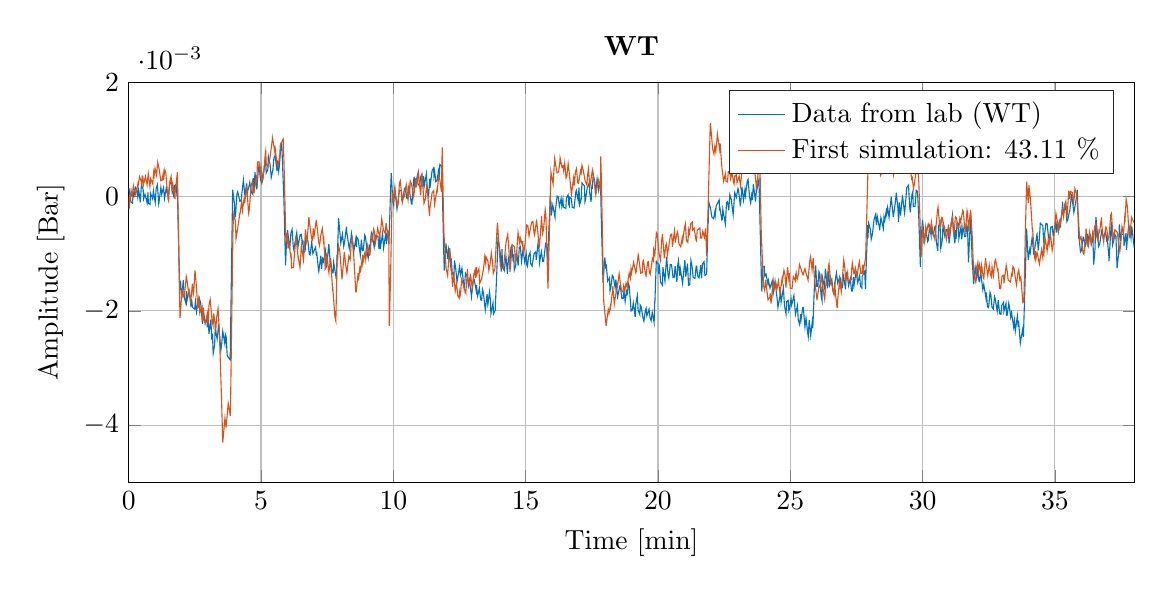
\begin{tikzpicture}

\begin{axis}[%
width=5.028in,
height=2in,
at={(1.011in,0.642in)},
scale only axis,
xmin=0,
xmax=38,
xlabel={Time [min]},
xmajorgrids,
ymin=-0.005,
ymax=0.002,
ylabel={Amplitude [Bar]},
ymajorgrids,
axis background/.style={fill=white},
title style={font=\bfseries},
title={WT},
legend style={legend cell align=left,align=left,draw=white!15!black}
]
\addplot [color=mycolor1,solid]
  table[row sep=crcr]{%
0.000833333333333333	8.51633431084853e-05\\
0.00833333333333333	0.000150412609970729\\
0.0816666666666667	-9.40546432063316e-05\\
0.143333333333333	-0.000117544379276413\\
0.168333333333333	8.34233626593184e-05\\
0.201666666666667	1.64341153476022e-05\\
0.26	0.000158242521994922\\
0.305833333333333	0.000127792864124399\\
0.343333333333333	-8.79560117406086e-06\\
0.375833333333333	0.000123442913000565\\
0.438333333333333	-0.0001027545454578\\
0.439166666666667	-7.83948191625805e-05\\
0.480833333333333	0.000205221994133087\\
0.546666666666667	0.000118222971652066\\
0.565	-4.01152492675305e-05\\
0.614166666666667	3.99238514169342e-05\\
0.696666666666667	-0.000111454447700943\\
0.731666666666667	7.47234604110136e-05\\
0.739166666666667	-0.000114934408601358\\
0.805833333333333	-0.000136684164220829\\
0.823333333333333	5.7323655914765e-05\\
0.904166666666667	-4.09852394930021e-05\\
0.931666666666667	0.00010430312805304\\
1.00083333333333	-0.000103624535678554\\
1.0375	0.000141712707722258\\
1.08416666666667	0.000207831964807531\\
1.135	-0.0001245043010768\\
1.14416666666667	-0.000100144574782024\\
1.21666666666667	0.000161722482890619\\
1.24666666666667	4.07938416402409e-05\\
1.315	0.000156502541546394\\
1.35333333333333	-3.14153470163114e-05\\
1.41916666666667	0.00015128260019398\\
1.46333333333333	3.64438905181008e-05\\
1.50833333333333	5.73236559149315e-05\\
1.54666666666667	0.000220881818184276\\
1.6075	0.000252201466277413\\
1.64166666666667	0.000102563147603707\\
1.695	1.64341153447711e-05\\
1.73416666666667	0.000192172140762392\\
1.79	0.000215661876830087\\
1.81833333333333	5.03637341123242e-05\\
1.84	7.82034213075156e-05\\
1.9275	-0.00163654731182694\\
1.9575	-0.00147037917888707\\
1.9975	-0.00179053558162812\\
2.06333333333333	-0.00146341925709653\\
2.10083333333333	-0.00176530586510201\\
2.15833333333333	-0.00186622473117726\\
2.18083333333333	-0.00165655708699564\\
2.19833333333333	-0.00182968514173953\\
2.27333333333333	-0.00164437722385946\\
2.2975	-0.00168439677419974\\
2.35333333333333	-0.00192712404692505\\
2.375	-0.00179488553275239\\
2.41166666666667	-0.00194191388075415\\
2.4925	-0.00196888357771588\\
2.5225	-0.00183490508308981\\
2.56166666666667	-0.00201847302053143\\
2.62083333333333	-0.00183142512218515\\
2.63	-0.00192886402736636\\
2.66	-0.00176269589442474\\
2.71916666666667	-0.00186361476051136\\
2.78666666666667	-0.00222814066472016\\
2.8175	-0.00197758347996801\\
2.88833333333333	-0.00222379071359588\\
2.96	-0.00210547204301781\\
2.9675	-0.00228816999022985\\
3	-0.00208807223851926\\
3.0325	-0.00240387869013778\\
3.10666666666667	-0.00215071153470978\\
3.135	-0.00250305757575964\\
3.16166666666667	-0.00239865874877754\\
3.19333333333333	-0.00274752482893481\\
3.245	-0.00260310645162026\\
3.26833333333333	-0.00231252971652074\\
3.3425	-0.00249261769305978\\
3.39916666666667	-0.00223597057673988\\
3.41916666666667	-0.00234558934506657\\
3.4825	-0.00269097546432623\\
3.51333333333333	-0.00257874672532088\\
3.55416666666667	-0.00235602922776357\\
3.63416666666667	-0.00258048670577216\\
3.6525	-0.0024125785923842\\
3.6825	-0.00245433812317292\\
3.7225	-0.00278493440860492\\
3.835	-0.00285888357772554\\
3.85333333333333	-0.00225598035191643\\
3.9275	0.000120832942317961\\
3.99333333333333	-0.000111454447713905\\
4.005	-0.000314162170098248\\
4.035	-0.000338521896390526\\
4.0875	3.81838709636872e-05\\
4.11833333333333	8.16833822107899e-05\\
4.20083333333333	-8.36147605013104e-05\\
4.25	-6.6214956008448e-05\\
4.28916666666667	0.000109523069397821\\
4.33416666666667	0.000289611045938998\\
4.37916666666667	5.81936461444832e-05\\
4.39	1.99140762576211e-05\\
4.45833333333333	0.000230451710646756\\
4.47416666666667	5.73236559149315e-05\\
4.55416666666667	0.000196522091886309\\
4.57333333333333	0.000247851515158104\\
4.64	7.55934506345146e-05\\
4.68916666666667	3.99238514320333e-05\\
4.72333333333333	0.000320930694040655\\
4.74416666666667	8.60333333378982e-05\\
4.76916666666667	0.000425329521002132\\
4.84083333333333	0.000125182893434439\\
4.89666666666667	0.000450559237515441\\
4.92416666666667	0.000543648191569546\\
4.98	0.000296570967729892\\
5.02666666666667	0.000239151612916641\\
5.07166666666667	0.000394009872933157\\
5.08416666666667	0.000374000097758759\\
5.16666666666667	0.000654136950139259\\
5.17	0.000702856402726687\\
5.19333333333333	0.000410539687187947\\
5.255	0.00046360909090179\\
5.27583333333333	0.000707206353861622\\
5.3425	0.000562787976548504\\
5.38666666666667	0.000333110557173305\\
5.45	0.00047056901268841\\
5.4875	0.000681106647100291\\
5.5325	0.000721126197459038\\
5.6025	0.000446209286401808\\
5.62333333333333	0.000632387194510031\\
5.6675	0.00043837937437427\\
5.69583333333333	0.000547128152484894\\
5.755	0.000932533822079154\\
5.78416666666667	0.000925573900283999\\
5.8675	-0.000103624535668589\\
5.92666666666667	-0.00120416217007308\\
5.96	-0.000818756500483075\\
6.00333333333333	-0.000589079081129179\\
6.08333333333333	-0.000923155327471559\\
6.12916666666667	-0.000636058553266039\\
6.17416666666667	-0.000576899217978072\\
6.21666666666667	-0.00087443587487418\\
6.24	-0.000930985239477766\\
6.305	-0.000751767253159036\\
6.35083333333333	-0.000629968621687627\\
6.3925	-0.000859646041048628\\
6.395	-0.000883135777118488\\
6.47916666666667	-0.000664768230686175\\
6.52	-0.000661288269780763\\
6.5675	-0.000841376246329073\\
6.58083333333333	-0.000756987194520664\\
6.61	-0.000983184652969177\\
6.66583333333333	-0.000954474975557562\\
6.69416666666667	-0.000753507233616696\\
6.77	-0.000770907038128044\\
6.82416666666667	-0.00101015434995436\\
6.85333333333333	-0.00102146422286598\\
6.91333333333333	-0.000798746725300142\\
6.92083333333333	-0.000813536559115757\\
6.9575	-0.000995364516104658\\
7.06083333333333	-0.000888355718450279\\
7.09166666666667	-0.00103538406645631\\
7.1025	-0.000970134799587075\\
7.17416666666667	-0.00129116119256442\\
7.1825	-0.00131117096773739\\
7.26166666666667	-0.00103277409581456\\
7.28666666666667	-0.00126419149560908\\
7.32666666666667	-0.00109367341151756\\
7.35666666666667	-0.00113804291298425\\
7.43916666666667	-0.000943165102634591\\
7.44333333333333	-0.000990144574774282\\
7.47666666666667	-0.00124505171064004\\
7.5625	-0.000829196383175107\\
7.61666666666667	-0.00117023255132542\\
7.625	-0.00108062355816532\\
7.685	-0.00133640068426777\\
7.72416666666667	-0.00133466070381436\\
7.745	-0.00115196275660015\\
7.84666666666667	-0.00145123939393688\\
7.87083333333333	-0.00102146422286598\\
7.88166666666667	-0.00109889335287353\\
7.93083333333333	-0.000375931476040037\\
7.97166666666667	-0.000594299022476624\\
8.01416666666667	-0.000815276539581938\\
8.07666666666667	-0.000655198338216589\\
8.125	-0.000872695894426456\\
8.1575	-0.000798746725315769\\
8.22833333333333	-0.000526439784937244\\
8.2325	-0.000594299022470934\\
8.31333333333333	-0.00085616608015035\\
8.33416666666667	-0.000911845454549975\\
8.4025	-0.000716097653975012\\
8.41833333333333	-0.000646498435997844\\
8.48666666666667	-0.00086312600195404\\
8.505	-0.000964914858249594\\
8.58166666666667	-0.000735237438905662\\
8.605	-0.000885745747785799\\
8.61666666666667	-0.000709137732141485\\
8.66916666666667	-0.000746547311814449\\
8.75083333333333	-0.0010258141739995\\
8.79166666666667	-0.000753507233622386\\
8.83083333333333	-0.000946645063538559\\
8.865	-0.000940555131958731\\
8.91916666666667	-0.000672598142708036\\
8.9475	-0.000700437829905698\\
9.01833333333333	-0.00100667438904897\\
9.04833333333333	-0.00107801358748238\\
9.1025	-0.000841376246324799\\
9.11	-0.000928375268807624\\
9.17083333333333	-0.000625618670556966\\
9.195	-0.000647368426186179\\
9.27583333333333	-0.000887485728244902\\
9.28416666666667	-0.000859646041052903\\
9.31833333333333	-0.000678688074290695\\
9.41916666666667	-0.000696087878802043\\
9.455	-0.000916195405690601\\
9.49166666666667	-0.000658678299137599\\
9.50333333333333	-0.000919675366577527\\
9.59333333333333	-0.000645628445761215\\
9.6325	-0.000897925610953976\\
9.7175	-0.000631708602148146\\
9.74	-0.000827456402751531\\
9.78333333333333	-0.000582119159361016\\
9.83333333333333	-0.000835286314781913\\
9.895	0.000110393059625929\\
9.9225	0.000414889638310101\\
9.97916666666667	-8.6224731208423e-05\\
10.0133333333333	-0.000159303910078179\\
10.0391666666667	3.557390030276e-05\\
10.0966666666667	-3.66352883758303e-05\\
10.1375	-0.000218463245369005\\
10.16	-0.000133204203339593\\
10.2291666666667	0.000103433137829345\\
10.3041666666667	0.000101693157373101\\
10.315	-5.66450635487992e-05\\
10.3408333333333	-9.14446725515938e-05\\
10.42	0.000136492766375895\\
10.4516666666667	0.000155632551334967\\
10.5058333333333	-2.53254154613525e-05\\
10.55	-3.75052786067975e-05\\
10.565	0.000169552394908234\\
10.5958333333333	0.000138232746823619\\
10.6833333333333	-0.000128854252190447\\
10.7025	-0.000133204203322523\\
10.7641666666667	0.000275691202324527\\
10.7866666666667	0.000346160410552548\\
10.8041666666667	0.000162592473125861\\
10.9175	0.000382699999994532\\
10.9291666666667	0.000225231769306444\\
10.9908333333333	0.000179992277605928\\
11.0333333333333	0.000345290420313046\\
11.0775	0.000392269892478328\\
11.1091666666667	0.000176512316738903\\
11.1433333333333	0.000358340273729246\\
11.1666666666667	0.000179122287431804\\
11.2491666666667	0.000398359824063832\\
11.2841666666667	0.000136492766395796\\
11.3325	2.60040078530754e-05\\
11.3775	0.000311360801575331\\
11.385	0.000153022580642065\\
11.4675	0.00046099912023588\\
11.5208333333333	0.000500148680339513\\
11.535	0.000360950244373826\\
11.5616666666667	0.000439249364618019\\
11.6041666666667	0.000258291397852967\\
11.6525	0.00027656119256686\\
11.7058333333333	0.000456649169112311\\
11.7408333333333	0.000377480058671248\\
11.7566666666667	0.00056278797655987\\
11.83	0.000527118377323277\\
11.9091666666667	-0.00106496373410597\\
11.9258333333333	-0.00129638113390901\\
11.9916666666667	-0.000819626490684205\\
11.9975	-0.00086312600193697\\
12.0575	-0.00109367341154032\\
12.0841666666667	-0.000933595210176358\\
12.1683333333333	-0.00122504193548698\\
12.1891666666667	-0.00108410351907073\\
12.225	-0.00133553069404957\\
12.2883333333333	-0.00138860009775205\\
12.3108333333333	-0.00111977311826753\\
12.3525	-0.00124244173999546\\
12.4083333333333	-0.0014903889540675\\
12.4341666666667	-0.0014146998044878\\
12.5025	-0.00122591192572363\\
12.5366666666667	-0.0013703303030268\\
12.5925	-0.00125462160310397\\
12.6091666666667	-0.00133727067446604\\
12.6758333333333	-0.00161392756596956\\
12.6975	-0.00151996862167028\\
12.7266666666667	-0.00134075063537001\\
12.7958333333333	-0.0013972999999935\\
12.8375	-0.00155911818180232\\
12.8733333333333	-0.00146167927663601\\
12.9533333333333	-0.00175225601170997\\
12.96	-0.00171223646135832\\
13.0191666666667	-0.00144862942324825\\
13.0525	-0.00144775943305139\\
13.13	-0.00164263724340674\\
13.1416666666667	-0.00155041827957508\\
13.1866666666667	-0.00173833616812535\\
13.2508333333333	-0.00160174770283267\\
13.2991666666667	-0.00180532541545222\\
13.3341666666667	-0.00181402531770222\\
13.3683333333333	-0.00162436744866729\\
13.4016666666667	-0.00167830684261208\\
13.4733333333333	-0.00198541339196642\\
13.5425	-0.00170440654935353\\
13.5708333333333	-0.00189580439882764\\
13.5725	-0.00189319442815181\\
13.6341666666667	-0.0016678669599286\\
13.6675	-0.00180967536656729\\
13.6866666666667	-0.00205153264906233\\
13.7666666666667	-0.00186361476051208\\
13.7883333333333	-0.00205066265886833\\
13.8491666666667	-0.00198976334312409\\
13.9225	-0.00117284252198135\\
13.9533333333333	-0.000701307820153735\\
14.0425	-0.000997104496579387\\
14.0758333333333	-0.00131552091885387\\
14.1075	-0.000917935386101382\\
14.125	-0.00123635180838721\\
14.1916666666667	-0.00129812111437946\\
14.2558333333333	-0.00104930391007929\\
14.3116666666667	-0.0013538004887379\\
14.3458333333333	-0.00107279364613636\\
14.4025	-0.00117632248290239\\
14.4433333333333	-0.000891835679388359\\
14.4825	-0.000859646041064255\\
14.5266666666667	-0.00113717292276466\\
14.5475	-0.00101363431083987\\
14.5716666666667	-0.00128681124146215\\
14.6233333333333	-0.00120677214076739\\
14.6566666666667	-0.000962304887551002\\
14.7175	-0.00120764213096994\\
14.76	-0.000889225708686936\\
14.8008333333333	-0.00087443587487418\\
14.8433333333333	-0.00113369296188059\\
14.8991666666667	-0.000937075171074664\\
14.965	-0.00114413284458398\\
15.02	-0.00099623450633704\\
15.0375	-0.0011911123166839\\
15.0691666666667	-0.00122330195500231\\
15.1091666666667	-0.00104843391982559\\
15.1683333333333	-0.000977094721417771\\
15.1866666666667	-0.00116849257089474\\
15.2425	-0.00121634203324836\\
15.3183333333333	-0.000999714467266599\\
15.3783333333333	-0.000970134799624045\\
15.4025	-0.00110933323559825\\
15.4141666666667	-0.00106148377323326\\
15.4658333333333	-0.000821366471154661\\
15.5008333333333	-0.000913585434986319\\
15.5241666666667	-0.00116240263927797\\
15.5941666666667	-0.000964044867990205\\
15.6483333333333	-0.0011389129032067\\
15.6758333333333	-0.00113804291297573\\
15.7575	-0.000814406549315444\\
15.7841666666667	-0.000816146529760337\\
15.8408333333333	-0.00113021300094818\\
15.8491666666667	-0.000897055620694587\\
15.925	-3.92452590317616e-05\\
15.955	-8.62247311487208e-05\\
15.9683333333333	-0.000330691984322479\\
16.0241666666667	-0.000149734017583003\\
16.1083333333333	-0.000359401661771036\\
16.1116666666667	-0.000285452492661764\\
16.1908333333333	8.60420332182699e-06\\
16.2341666666667	-4.44565005741637e-06\\
16.275	-0.000170613782969897\\
16.3391666666667	-3.40253176857597e-05\\
16.3666666666667	-0.000168873802542074\\
16.4083333333333	-4.70751710905937e-05\\
16.4258333333333	-0.000184533626631289\\
16.5191666666667	-0.000208023362657073\\
16.54	-2.09754643008264e-05\\
16.605	3.20939394101716e-05\\
16.6283333333333	-0.000140164125102066\\
16.6483333333333	-0.000163653861173341\\
16.6625	-1.22755620622084e-05\\
16.7275	-3.40253176857597e-05\\
16.7608333333333	-0.000188013587469893\\
16.8308333333333	-0.000200193450675012\\
16.8966666666667	8.69033234750793e-05\\
16.9141666666667	0.000108653079129883\\
16.9825	-6.70849462635625e-05\\
17.0158333333333	0.000153892570833231\\
17.0425	-0.000140164125187331\\
17.0991666666667	-4.44652004459867e-05\\
17.1275	0.000238281622617464\\
17.2208333333333	0.000186952199376922\\
17.2416666666667	-9.05746823348375e-05\\
17.2583333333333	-6.09950146695237e-05\\
17.325	0.000146932649070758\\
17.4066666666667	0.000245241544448146\\
17.42	6.51535679225823e-05\\
17.4725	-9.40546432075529e-05\\
17.5033333333333	0.000202612023477489\\
17.5141666666667	0.000133882795714246\\
17.5541666666667	0.000384439980476353\\
17.61	0.000260031378255227\\
17.6425	4.60137829606799e-05\\
17.7	0.000311360801563965\\
17.76	0.000106043108442672\\
17.8258333333333	0.000316580742898614\\
17.8625	-0.000464670479001839\\
17.9233333333333	-0.00150778875857033\\
17.9916666666667	-0.00106583372437105\\
18.0316666666667	-0.00126680146629771\\
18.0458333333333	-0.0011867623656342\\
18.0975	-0.00147994907138971\\
18.1658333333333	-0.00142252971654944\\
18.1891666666667	-0.00165307712611298\\
18.2183333333333	-0.00159478778107019\\
18.2733333333333	-0.00137816021509413\\
18.31	-0.00140686989248298\\
18.3816666666667	-0.00159652776159466\\
18.4083333333333	-0.00145210938425455\\
18.475	-0.00175660596284208\\
18.4808333333333	-0.00174529608991908\\
18.5583333333333	-0.00156172815254924\\
18.5733333333333	-0.0015573782013944\\
18.635	-0.00178444565001135\\
18.6858333333333	-0.00178270566967445\\
18.7183333333333	-0.00163567732165282\\
18.76	-0.00184012502443512\\
18.8233333333333	-0.00162523743894372\\
18.8325	-0.00173485620727254\\
18.8858333333333	-0.00152344858261974\\
18.9141666666667	-0.00156694809384977\\
18.9841666666667	-0.00200368318669736\\
19.0275	-0.00198802336266501\\
19.0675	-0.00186448475072032\\
19.1391666666667	-0.00210460205276763\\
19.1566666666667	-0.00189319442812053\\
19.2216666666667	-0.00173659618768329\\
19.2483333333333	-0.00198454340176388\\
19.315	-0.00206632248297456\\
19.3283333333333	-0.00189841436956317\\
19.3641666666667	-0.00192538406651854\\
19.4358333333333	-0.00212461182797188\\
19.4691666666667	-0.00218290117295783\\
19.5191666666667	-0.00200542316711949\\
19.5525	-0.00195583372432953\\
19.5791666666667	-0.00208894222874667\\
19.6633333333333	-0.00197149354837325\\
19.7008333333333	-0.00212287184745311\\
19.7433333333333	-0.00217333128051383\\
19.7841666666667	-0.00202804291302233\\
19.855	-0.00220552091884363\\
19.8766666666667	-0.00185056490713853\\
19.8833333333333	-0.00185317487780867\\
19.9366666666667	-0.00113282297169509\\
20.0041666666667	-0.00117371251224929\\
20.0158333333333	-0.00135119051814447\\
20.055	-0.00123722179871766\\
20.1033333333333	-0.00149995884659393\\
20.17	-0.00155215826004271\\
20.1866666666667	-0.00123722179865515\\
20.2633333333333	-0.00147907908119282\\
20.3141666666667	-0.00113978289346894\\
20.3258333333333	-0.00105191388076084\\
20.3825	-0.00137729022485178\\
20.4091666666667	-0.00142600967747331\\
20.465	-0.00118850234608478\\
20.5116666666667	-0.00119024232651829\\
20.5683333333333	-0.00141643978498385\\
20.6108333333333	-0.00141730977519205\\
20.6483333333333	-0.00121721202346795\\
20.7133333333333	-0.00149386891495443\\
20.7475	-0.00120155219942991\\
20.7741666666667	-0.0011206431085127\\
20.8208333333333	-0.00138425014664836\\
20.8441666666667	-0.00126419149561049\\
20.9133333333333	-0.00147385913986386\\
20.93	-0.00152170860223738\\
21.015	-0.00111803313784822\\
21.0158333333333	-0.00111194320627125\\
21.0508333333333	-0.00139903998046112\\
21.115	-0.00117284252204106\\
21.155	-0.00155302825025094\\
21.2	-0.00154345835777281\\
21.245	-0.00111890312805646\\
21.2908333333333	-0.00123026187681877\\
21.3283333333333	-0.00141295982403722\\
21.3966666666667	-0.00143296959923012\\
21.445	-0.00121547204304012\\
21.4641666666667	-0.0012172120234509\\
21.4958333333333	-0.00138599012706483\\
21.5508333333333	-0.00142339970674632\\
21.6158333333333	-0.00119981221904755\\
21.6441666666667	-0.00142948963838013\\
21.685	-0.00117806246343821\\
21.7433333333333	-0.00114152287395361\\
21.7733333333333	-0.00137903020526825\\
21.8391666666667	-0.00135554046928793\\
21.8891666666667	-0.00044031075277351\\
21.8958333333333	-0.000477720332449305\\
21.9216666666667	-9.66646139629601e-05\\
21.9841666666667	-0.000202803421390646\\
22.04	-0.000363751612965646\\
22.1016666666667	-0.000386371358794602\\
22.15	-0.000269792668714686\\
22.1633333333333	-0.000327212023515155\\
22.2033333333333	-0.000159303910126501\\
22.3133333333333	-5.92550343042342e-05\\
22.3225	-0.000244562952181476\\
22.3333333333333	-0.00017409374395061\\
22.4125	-0.000408991104691725\\
22.4291666666667	-0.000399421212224998\\
22.45	-0.000225423167208194\\
22.5466666666667	-0.00047772033236404\\
22.5908333333333	-0.000105364516147594\\
22.6258333333333	-8.88347018672131e-05\\
22.6766666666667	-0.000241952981443111\\
22.6783333333333	-0.000216723264921281\\
22.7141666666667	3.38339198124038e-05\\
22.7658333333333	-4.09852395334975e-05\\
22.8408333333333	-0.000316772140800392\\
22.8575	-0.00022020322583946\\
22.9008333333333	6.77635385700204e-05\\
22.96	-1.57555230116679e-05\\
23.0233333333333	0.000139102736980701\\
23.0433333333333	0.000113003030239256\\
23.1083333333333	-0.000146254056696105\\
23.1258333333333	-0.000113194428152386\\
23.1716666666667	0.000172162365541434\\
23.2316666666667	-6.36049853226517e-05\\
23.2841666666667	0.000113873020498645\\
23.3033333333333	1.90440860053376e-05\\
23.3758333333333	0.000276561192603803\\
23.4041666666667	0.000300050928680767\\
23.4583333333333	5.12424236670528e-06\\
23.5041666666667	-0.000112324438006683\\
23.5533333333333	7.90734114930192e-05\\
23.57	-5.75150537911462e-05\\
23.6041666666667	0.000215661876811268\\
23.6875	-8.97046921550237e-05\\
23.7275	0.000221751808365506\\
23.7341666666667	0.000112133040031021\\
23.8166666666667	0.000300920918809414\\
23.9041666666667	-0.00139382003909239\\
23.925	-0.00166438699899618\\
23.9541666666667	-0.00123200185726935\\
24.015	-0.00122069198435204\\
24.0375	-0.00139208005867023\\
24.0841666666667	-0.00135554046919129\\
24.1541666666667	-0.00153040850445041\\
24.1741666666667	-0.0014668992180332\\
24.2341666666667	-0.00160348768322638\\
24.3175	-0.00147559912018938\\
24.3408333333333	-0.00168526676439729\\
24.3466666666667	-0.00171571642225377\\
24.4241666666667	-0.0014790790811019\\
24.4291666666667	-0.00149908885628908\\
24.5075	-0.00180967536659571\\
24.5333333333333	-0.00193930391007191\\
24.6041666666667	-0.00175225601168155\\
24.6208333333333	-0.00161566754638603\\
24.6508333333333	-0.00184969491687345\\
24.74	-0.00159826774194291\\
24.7791666666667	-0.0019062442815623\\
24.8391666666667	-0.00205675259051918\\
24.8625	-0.00183751505384455\\
24.9208333333333	-0.00181750527863461\\
24.9441666666667	-0.00200281319654028\\
24.9641666666667	-0.00197584349953947\\
25.0283333333333	-0.00178531564028209\\
25.0516666666667	-0.00189754437930947\\
25.1158333333333	-0.00177748572827161\\
25.1366666666667	-0.00173224623659099\\
25.195	-0.00206284252199385\\
25.27	-0.00190972424243502\\
25.3008333333333	-0.00215767145653833\\
25.3533333333333	-0.00224119051813138\\
25.3925	-0.00205675259047372\\
25.41	-0.00214549159337299\\
25.4716666666667	-0.00194191388078754\\
25.4925	-0.00194104389059635\\
25.5541666666667	-0.00228208005868558\\
25.595	-0.00212809178889575\\
25.6508333333333	-0.00236385913983372\\
25.6791666666667	-0.00244998817205716\\
25.715	-0.00215854144671812\\
25.7708333333333	-0.00243606832847537\\
25.83	-0.00219595102642803\\
25.8516666666667	-0.00230382981425512\\
25.9175	-0.00147994907136129\\
25.9591666666667	-0.00120416217011712\\
26.0008333333333	-0.00157303802541539\\
26.0391666666667	-0.00157303802536424\\
26.0833333333333	-0.00131378093841183\\
26.0991666666667	-0.00133379071358763\\
26.165	-0.00173920615830231\\
26.1991666666667	-0.00182011524925929\\
26.2158333333333	-0.00141469980453326\\
26.2925	-0.00159043782990967\\
26.3266666666667	-0.00126332150538522\\
26.41	-0.00160522766376223\\
26.4333333333333	-0.00132161085042801\\
26.455	-0.00131639090909905\\
26.4816666666667	-0.00155911818181087\\
26.5691666666667	-0.00144949941355596\\
26.6183333333333	-0.00166351700885617\\
26.6541666666667	-0.00169918660801319\\
26.7016666666667	-0.00146080928637662\\
26.7441666666667	-0.00133727067450015\\
26.7933333333333	-0.00151648866082885\\
26.8608333333333	-0.00141121984365489\\
26.8741666666667	-0.00162262746829062\\
26.8933333333333	-0.00141556979475854\\
26.9416666666667	-0.00160087771255624\\
26.9758333333333	-0.00159043782990398\\
27.0033333333333	-0.00135554046924247\\
27.0866666666667	-0.00162349745848747\\
27.1175	-0.00133118074295158\\
27.1508333333333	-0.00134858054741177\\
27.2033333333333	-0.00155911818185633\\
27.2675	-0.00143470957971478\\
27.3141666666667	-0.00165394711638944\\
27.3416666666667	-0.00165220713592182\\
27.3858333333333	-0.00140686989251709\\
27.4091666666667	-0.00155563822094951\\
27.4925	-0.00130160107533744\\
27.4933333333333	-0.00131552091893061\\
27.5466666666667	-0.00150865874878425\\
27.6208333333333	-0.00138164017600662\\
27.6516666666667	-0.00157216803522989\\
27.7041666666667	-0.00160174770286109\\
27.7175	-0.00139643000980233\\
27.8091666666667	-0.0013103009774709\\
27.8416666666667	-0.00161914750729852\\
27.8441666666667	-0.00152344858257994\\
27.925	-0.000502080058671944\\
27.9333333333333	-0.000727407526917911\\
27.9625	-0.000469020430139633\\
28.0233333333333	-0.000570809286429497\\
28.0583333333333	-0.000745677321643157\\
28.1066666666667	-0.000648238416519481\\
28.1625	-0.000409861094848807\\
28.2166666666667	-0.000322862072377361\\
28.2575	-0.000501210068486468\\
28.2816666666667	-0.000335911925762294\\
28.3683333333333	-0.000548189540589217\\
28.3758333333333	-0.00059168905182494\\
28.4241666666667	-0.000367231573861093\\
28.5166666666667	-0.000560369403765915\\
28.5408333333333	-0.000357661681371635\\
28.57	-0.0004168210165999\\
28.6275	-0.000251522873898485\\
28.645	-0.00031242218968533\\
28.6783333333333	-0.00019323352890116\\
28.7325	-0.000363751612948604\\
28.8066666666667	-4.62051809306807e-05\\
28.8108333333333	-1.83567945830077e-06\\
28.8941666666667	-0.000361141642261392\\
28.895	-0.000353311730239531\\
28.98	-6.53449658130079e-05\\
29.0066666666667	6.77635385814002e-05\\
29.07	-0.000227163147630355\\
29.0908333333333	-0.000442920723392498\\
29.1191666666667	-0.000103624535725433\\
29.165	-0.000332431964804314\\
29.2358333333333	-9.65689153420435e-07\\
29.2483333333333	-1.83654936590782e-05\\
29.3183333333333	-0.000287192473214654\\
29.3383333333333	-0.000205413392077858\\
29.4008333333333	0.000154762561035776\\
29.4683333333333	0.000197392082057601\\
29.5075	-0.000146254056690415\\
29.5341666666667	-0.000276752590437357\\
29.5941666666667	3.03539589169566e-05\\
29.63	8.51633431097898e-05\\
29.6483333333333	-0.000174963734113381\\
29.7133333333333	-0.000172353763522787\\
29.7591666666667	0.00010952306938361\\
29.8075	8.95132942589361e-05\\
29.8575	-0.00039942121208289\\
29.9158333333333	-0.0012293918866276\\
29.945	-0.000743067350967297\\
29.9966666666667	-0.000408121114443716\\
30.0341666666667	-0.000585599120282054\\
30.0541666666667	-0.000823976441861773\\
30.1266666666667	-0.00058646911047322\\
30.1883333333333	-0.000788306842596759\\
30.2125	-0.000767427077224075\\
30.2616666666667	-0.000530789736089221\\
30.3225	-0.000683908015699231\\
30.3333333333333	-0.000543839589502576\\
30.4008333333333	-0.000676948093857183\\
30.4675	-0.000522089833773887\\
30.485	-0.000517739882658824\\
30.5191666666667	-0.000795266764359231\\
30.5741666666667	-0.000951865004927194\\
30.6033333333333	-0.000523829814332438\\
30.6575	-0.000444660703854433\\
30.6866666666667	-0.000903145552339779\\
30.7391666666667	-0.000774386999043392\\
30.77	-0.000513389931629055\\
30.8391666666667	-0.000694347898425374\\
30.9058333333333	-0.000580379178930363\\
30.9525	-0.000573419257139468\\
30.9958333333333	-0.000768297067517576\\
31	-0.000822236461456682\\
31.0833333333333	-0.000472500390983899\\
31.13	-0.000321992082089551\\
31.1683333333333	-0.000623878690160395\\
31.22	-0.000817886510307536\\
31.2408333333333	-0.000586469110507332\\
31.2625	-0.00074393734116418\\
31.3041666666667	-0.000449880645172041\\
31.3458333333333	-0.000471630400821155\\
31.3708333333333	-0.000736107429176402\\
31.4525	-0.000522959824124203\\
31.4791666666667	-0.000750027272803683\\
31.5233333333333	-0.000535139687249747\\
31.5891666666667	-0.000701307820182157\\
31.6283333333333	-0.000697827859286709\\
31.6725	-0.000509039980462839\\
31.6983333333333	-0.000548189540566457\\
31.7341666666667	-0.0011519627565888\\
31.815	-0.000286322482921153\\
31.8716666666667	-0.00110933323557266\\
31.875	-0.00110063333333121\\
31.9266666666667	-0.0015321484848555\\
31.985	-0.00123374183774833\\
32.0433333333333	-0.00142861964815486\\
32.0775	-0.00128507126105706\\
32.13	-0.0014799490713556\\
32.1533333333333	-0.00148864897357431\\
32.1925	-0.00130682101657545\\
32.23	-0.00145819931577468\\
32.2758333333333	-0.00162697741937723\\
32.3108333333333	-0.00153649843599898\\
32.3941666666667	-0.00177835571850257\\
32.4116666666667	-0.00167569687198171\\
32.4508333333333	-0.00193234398826395\\
32.4933333333333	-0.00194713382210512\\
32.5475	-0.00167569687202151\\
32.5783333333333	-0.00171658641258138\\
32.625	-0.0019445238514236\\
32.6708333333333	-0.00196888357768035\\
32.72	-0.00175399599221171\\
32.7466666666667	-0.00179227556211278\\
32.8191666666667	-0.0020089031281002\\
32.8575	-0.00181141534704626\\
32.9108333333333	-0.00205066265882853\\
32.9591666666667	-0.00206110254153191\\
32.9925	-0.00190624428155095\\
33.0591666666667	-0.00185143489740358\\
33.0708333333333	-0.00201064310853941\\
33.1508333333333	-0.00187057468227456\\
33.1725	-0.00207937233625149\\
33.1925	-0.00207763235581229\\
33.2558333333333	-0.00186622473121634\\
33.2725	-0.00190972424247482\\
33.3283333333333	-0.00210982199417051\\
33.36	-0.0020315228739064\\
33.4408333333333	-0.00228208005869124\\
33.4691666666667	-0.00216985131964681\\
33.5033333333333	-0.0023551592375127\\
33.5808333333333	-0.00209155219945092\\
33.6108333333333	-0.00228034007817246\\
33.6258333333333	-0.00217420127075049\\
33.6925	-0.00256569687195157\\
33.71	-0.00251175747800678\\
33.7775	-0.00233079951123888\\
33.8091666666667	-0.00245781808402787\\
33.885	-0.00130508103618174\\
33.9291666666667	-0.000562109384222159\\
33.9891666666667	-0.00110759325512777\\
34.0483333333333	-0.000922285337182305\\
34.0683333333333	-0.000975354740873402\\
34.1375	-0.000719577614981315\\
34.1516666666667	-0.000771777028475529\\
34.1941666666667	-0.000984054643274029\\
34.24	-0.000907495503437772\\
34.3233333333333	-0.000656068328461767\\
34.3241666666667	-0.000655198338242152\\
34.37	-0.000942295112358132\\
34.4116666666667	-0.000737847409479186\\
34.4475	-0.000465540469096387\\
34.5433333333333	-0.000512519941386708\\
34.5716666666667	-0.000769167057725784\\
34.6025	-0.000692607917900906\\
34.66	-0.000471630400849576\\
34.71	-0.00048033030302283\\
34.7541666666667	-0.00070217781036197\\
34.7883333333333	-0.00076481710646864\\
34.845	-0.00053600967727041\\
34.9	-0.000524699804449719\\
34.9341666666667	-0.000696957869055742\\
34.9358333333333	-0.000683038025462573\\
35.0225	-0.000455100586438467\\
35.0516666666667	-0.000630838611866025\\
35.0925	-0.000416821016526014\\
35.1291666666667	-0.000621268719427692\\
35.1983333333333	-0.000458580547350956\\
35.2058333333333	-0.000542969599152232\\
35.285	-0.000146254056480083\\
35.2875	-8.88347016341495e-05\\
35.3216666666667	-0.000301112316580449\\
35.4066666666667	-0.000149734017608594\\
35.4516666666667	-0.000438570772277463\\
35.4891666666667	-0.00040464115341754\\
35.5491666666667	-0.000252392863975964\\
35.56	-0.000255002834668866\\
35.6333333333333	5.12337243919747e-05\\
35.6366666666667	1.29541545022538e-05\\
35.7166666666667	-0.00028023255111681\\
35.7333333333333	-0.000237603030140476\\
35.8116666666667	-2.53254155238858e-05\\
35.8458333333333	0.00011474301070688\\
35.8966666666667	-0.000673468132921934\\
35.8991666666667	-0.000669118181812589\\
35.9666666666667	-0.000969264809313475\\
36.0033333333333	-0.000942295112369512\\
36.0666666666667	-0.000710007722406564\\
36.0825	-0.000712617693122197\\
36.15	-0.000862256011836759\\
36.1741666666667	-0.000831806353912057\\
36.2358333333333	-0.000649978396856349\\
36.2508333333333	-0.000884875757546311\\
36.3091666666667	-0.000648238416326219\\
36.3366666666667	-0.000672598142668235\\
36.3733333333333	-0.00083180635378699\\
36.4333333333333	-0.000685647996098632\\
36.4641666666667	-0.00119111231684588\\
36.5166666666667	-0.000910105474107942\\
36.5483333333333	-0.000355921700858519\\
36.6116666666667	-0.000682168035163411\\
36.6541666666667	-0.000873565884714267\\
36.6958333333333	-0.000820496480898103\\
36.7683333333333	-0.000595169012669206\\
36.7791666666667	-0.000602998924713827\\
36.8258333333333	-0.000736107429039984\\
36.9091666666667	-0.000623008699741856\\
36.9483333333333	-0.000749157282447649\\
36.9725	-0.000700437829877276\\
37.0358333333333	-0.00103799403700283\\
37.0433333333333	-0.00112934301064049\\
37.125	-0.0004986000976685\\
37.1275	-0.000442050733064914\\
37.18	-0.000845726197516578\\
37.2175	-0.000777866959944529\\
37.265	-0.0006673782012597\\
37.3066666666667	-0.000700437829809081\\
37.3483333333333	-0.00125549159327809\\
37.3975	-0.00103277409575345\\
37.4341666666667	-0.000487290224813725\\
37.4858333333333	-0.000783086901205265\\
37.505	-0.000659548289283302\\
37.5991666666667	-0.000661288269756616\\
37.6075	-0.00086834594327162\\
37.6883333333333	-0.000641278494637632\\
37.7058333333333	-0.000931855229734324\\
37.7375	-0.000736107429085475\\
37.79	-0.000484680254109443\\
37.8741666666667	-0.000727407526821267\\
37.9033333333333	-0.000523829814207399\\
38	-0.000904885532688027\\
};
\addlegendentry{Data from lab (WT)};

\addplot [color=mycolor2,solid]
  table[row sep=crcr]{%
0.000833333333333333	0\\
0.0166666666666667	-0.000209840502144356\\
0.0891666666666667	0.000107880315869561\\
0.1325	-5.75154506787214e-06\\
0.176666666666667	0.000180084570063946\\
0.178333333333333	0.000193197781537019\\
0.264166666666667	3.37638671365791e-05\\
0.351666666666667	0.000233696995751179\\
0.3625	0.000217946900824711\\
0.410833333333333	0.000345824740738254\\
0.493333333333333	0.000232848064028351\\
0.51	0.000358184581631045\\
0.533333333333333	0.000355473512933884\\
0.558333333333333	0.000206202225684672\\
0.634166666666667	0.000355199988531355\\
0.694166666666667	0.000207050875071455\\
0.701666666666667	0.000240926960180014\\
0.74	0.000400877184258196\\
0.8025	0.000176285503670862\\
0.831666666666667	0.000313441312007965\\
0.908333333333333	0.000222219785701946\\
0.945	0.000430102653240481\\
0.965	0.000376835302445917\\
0.995	0.000495666539219543\\
1.05333333333333	0.000373107420579453\\
1.09666666666667	0.000597590518293626\\
1.14583333333333	0.000493369588840034\\
1.21416666666667	0.000276867328354868\\
1.25666666666667	0.000278237773351007\\
1.30333333333333	0.000398028494150032\\
1.31583333333333	0.000287668013951483\\
1.36416666666667	0.000469473420380745\\
1.4025	0.000408760358986621\\
1.485	-3.92095886274585e-05\\
1.5075	-7.31921158367453e-05\\
1.54666666666667	0.000247973638319535\\
1.60166666666667	0.000351162097838841\\
1.63333333333333	0.000128832390448378\\
1.665	0.000226255399718813\\
1.74833333333333	-4.27044156145995e-05\\
1.7525	5.59201154610086e-05\\
1.84	0.000428075967076321\\
1.9275	-0.00186913303905048\\
1.93916666666667	-0.00212718838620172\\
2.0125	-0.00165673546889091\\
2.02083333333333	-0.00160284081029491\\
2.0625	-0.00175564266008258\\
2.1025	-0.00173656988071212\\
2.17583333333333	-0.00139928255215658\\
2.19	-0.00142769316178685\\
2.2725	-0.00170644311267252\\
2.28833333333333	-0.00165702930933545\\
2.34083333333333	-0.00185322984745202\\
2.40666666666667	-0.00152438302646647\\
2.43916666666667	-0.00170879703571385\\
2.46083333333333	-0.00163808965789746\\
2.505	-0.00129145326610493\\
2.54416666666667	-0.0014920074484405\\
2.61416666666667	-0.00195589681959578\\
2.65583333333333	-0.00175163888184472\\
2.68666666666667	-0.00204249275340661\\
2.76916666666667	-0.00191961173571666\\
2.7925	-0.00216987672837054\\
2.82166666666667	-0.00194248685377027\\
2.85	-0.00219496025144843\\
2.90416666666667	-0.00221577054858908\\
2.96916666666667	-0.00204421678711052\\
2.995	-0.00223432459282705\\
3.03333333333333	-0.00190318662767996\\
3.07916666666667	-0.00179934842653621\\
3.15166666666667	-0.00218030164912353\\
3.19	-0.00225598066519658\\
3.20916666666667	-0.0020471969859823\\
3.29333333333333	-0.00232126242130626\\
3.31916666666667	-0.00212294052776185\\
3.37666666666667	-0.00196365990164301\\
3.415	-0.00225906829558106\\
3.41666666666667	-0.00224835727548603\\
3.50333333333333	-0.00348415499105655\\
3.50416666666667	-0.00347854026210686\\
3.55333333333333	-0.00430437279921761\\
3.63666666666667	-0.00387720426531634\\
3.67833333333333	-0.00403593432541028\\
3.67916666666667	-0.00404474067423778\\
3.76	-0.00362004186295942\\
3.84	-0.00384202771304588\\
3.85333333333333	-0.00348449899417616\\
3.94166666666667	-0.000528370388984871\\
3.97083333333333	-0.000305231926660332\\
4.02916666666667	-0.000423740461756795\\
4.055	-0.000735467677643868\\
4.11833333333333	-0.00055600928721471\\
4.20166666666667	-0.000284994751639586\\
4.20416666666667	-0.000309418424918757\\
4.26666666666667	-8.83474219640091e-05\\
4.29916666666667	-0.000245005126178684\\
4.36333333333333	-1.50950410615669e-05\\
4.37916666666667	-0.000118159098609449\\
4.4625	0.000179806804221228\\
4.46833333333333	0.000138196485129926\\
4.5275	-0.000292218743559361\\
4.55416666666667	-0.000239700003573546\\
4.62916666666667	0.000196047838217507\\
4.6775	0.000273795974704293\\
4.70416666666667	7.75672190117921e-05\\
4.73333333333333	6.83478134603224e-05\\
4.81666666666667	0.000327679155964534\\
4.84416666666667	0.000265157144643817\\
4.86333333333333	0.000604251584069269\\
4.925	0.000603975359845132\\
4.96666666666667	0.000412053659328721\\
4.99833333333333	0.000516911223967106\\
5.03916666666667	0.000248920504601563\\
5.08083333333333	0.000317168183996292\\
5.16666666666667	0.000774965750419264\\
5.17666666666667	0.00080301411264958\\
5.19666666666667	0.000561105643859131\\
5.26916666666667	0.000519538083300973\\
5.3425	0.000688735438063194\\
5.43	0.00100963755806753\\
5.43166666666667	0.00102738022590047\\
5.51	0.000815854023270328\\
5.52166666666667	0.00089179299877414\\
5.6025	0.000571297695489329\\
5.64	0.00052403638927168\\
5.6925	0.000675830920840931\\
5.69666666666667	0.000616321368437598\\
5.7275	0.000896534261111072\\
5.8375	0.00100696035778309\\
5.8675	0.00061133090544089\\
5.94166666666667	-0.000819134839567813\\
5.98416666666667	-0.000631120082032767\\
6.02333333333333	-0.000911066545144563\\
6.05166666666667	-0.000806781066509905\\
6.12916666666667	-0.00106181259587745\\
6.13916666666667	-0.0010435937091652\\
6.15666666666667	-0.00125040341559362\\
6.22416666666667	-0.00123892447569375\\
6.305	-0.000787837398930417\\
6.31583333333333	-0.000688304811419517\\
6.3925	-0.00102589593952016\\
6.39333333333333	-0.00102220360231855\\
6.47166666666667	-0.00124490283402214\\
6.48	-0.00119415828284217\\
6.525	-0.000853808716528763\\
6.6025	-0.00110782653274075\\
6.65583333333333	-0.000778369984419205\\
6.68166666666667	-0.000573807687096542\\
6.72583333333333	-0.000790115578866696\\
6.74666666666667	-0.000745678125494317\\
6.80916666666667	-0.000360890186702405\\
6.83416666666667	-0.000462441970149374\\
6.90916666666667	-0.00072939393441995\\
6.94916666666667	-0.000760759515283468\\
6.97166666666667	-0.000558403279448727\\
7.00666666666667	-0.000683680646967443\\
7.085	-0.000420795633537562\\
7.095	-0.000424787561700808\\
7.18	-0.000796058580473978\\
7.2125	-0.000858695047627641\\
7.2675	-0.000653812883379484\\
7.3175	-0.000559793813526545\\
7.355	-0.000743161984771962\\
7.3675	-0.000692593843867047\\
7.42583333333333	-0.00127035156310209\\
7.45	-0.00125347634363744\\
7.47416666666667	-0.000992910511269121\\
7.565	-0.0013330769253866\\
7.61333333333333	-0.00111022934677323\\
7.62916666666667	-0.00113202952622259\\
7.70583333333333	-0.00161962271645806\\
7.71416666666667	-0.00161305076336038\\
7.79333333333333	-0.0021097605483752\\
7.8275	-0.00217600757208027\\
7.87666666666667	-0.00106327913854796\\
7.89333333333333	-0.0011236758940175\\
7.92916666666667	-0.000860051097358954\\
7.97666666666667	-0.000954141390184578\\
8.05416666666667	-0.00141123946131039\\
8.0625	-0.00144667132784963\\
8.14416666666667	-0.000982701187668639\\
8.14666666666667	-0.000968854005723074\\
8.2025	-0.00120851412011071\\
8.245	-0.00133319335524838\\
8.31916666666667	-0.00104509877020655\\
8.36833333333333	-0.00110496453744024\\
8.40666666666667	-0.000826542471530771\\
8.445	-0.000735566768287146\\
8.49333333333333	-0.000995666362376861\\
8.4975	-0.000978686631311492\\
8.58166666666667	-0.00166862895915206\\
8.595	-0.00167079989053358\\
8.66916666666667	-0.00133770532933793\\
8.6825	-0.00147193314260749\\
8.74083333333333	-0.0012102007584213\\
8.75666666666667	-0.0013285237149311\\
8.84166666666667	-0.0010177900277267\\
8.85	-0.001160818350167\\
8.93166666666667	-0.000970937872355824\\
8.95666666666667	-0.00110232493124203\\
8.99916666666667	-0.000937454237198179\\
9.03166666666667	-0.000850630015956794\\
9.08916666666667	-0.00103111739305882\\
9.115	-0.00102561154631021\\
9.17166666666667	-0.000700930136962853\\
9.21	-0.000763025201994393\\
9.25833333333333	-0.000569613817026626\\
9.29	-0.000619902127271183\\
9.32333333333333	-0.000808705334175894\\
9.37166666666667	-0.000693722072146739\\
9.40666666666667	-0.000555671445247908\\
9.48416666666667	-0.000694750643550572\\
9.54416666666667	-0.000483206257015757\\
9.56083333333333	-0.000391317036694096\\
9.6325	-0.000592514801483979\\
9.69083333333333	-0.000644456165242393\\
9.72	-0.000508610298048202\\
9.72583333333333	-0.000462125700978821\\
9.8075	-0.000728422827328088\\
9.82666666666667	-0.000597431404979551\\
9.84666666666667	-0.00226453568763501\\
9.895	-0.00141116840974952\\
9.955	6.8068465331926e-05\\
10	-5.97880824114613e-05\\
10.0575	0.00017254790918761\\
10.0766666666667	8.39080446864885e-05\\
10.145	-0.000168446749570002\\
10.18	-0.000147345042743525\\
10.2283333333333	0.000230316793546864\\
10.2625	0.000276484454125755\\
10.3325	-4.19404972066702e-05\\
10.34	-9.30331137196726e-05\\
10.39	3.76308922921258e-05\\
10.4208333333333	9.0055086056104e-06\\
10.4891666666667	0.000202665068677642\\
10.5558333333333	-4.87548377336965e-05\\
10.5916666666667	0.000162907924170121\\
10.6183333333333	6.80006313514636e-05\\
10.6408333333333	0.000274213902059463\\
10.6833333333333	0.000224840754890605\\
10.77	-4.10692393823465e-06\\
10.7708333333333	2.24148358112289e-06\\
10.8508333333333	0.000321574282642009\\
10.8666666666667	0.000163072026168247\\
10.9416666666667	0.00039916480017367\\
10.9491666666667	0.000423694133520883\\
11.0308333333333	2.29743239910004e-05\\
11.0333333333333	3.5431307779658e-05\\
11.085	0.000391825868194775\\
11.1208333333333	0.00014698073253785\\
11.1583333333333	-0.000117486569577927\\
11.2183333333333	-3.32033710629113e-05\\
11.255	0.000218301723090612\\
11.2958333333333	4.80573060989394e-05\\
11.3658333333333	-0.000335557553412972\\
11.3833333333333	-0.00020248545218957\\
11.4666666666667	7.03097723740423e-05\\
11.5233333333333	0.000103027183090054\\
11.5583333333333	-0.000134694051949272\\
11.6425	0.000107016488935347\\
11.6508333333333	5.44748308269593e-05\\
11.7166666666667	0.000369203890479186\\
11.7575	0.000289596717059612\\
11.8183333333333	7.92693911887747e-05\\
11.8458333333333	0.000860164176702802\\
11.9091666666667	-0.000625738884291447\\
11.9925	-0.00125966958065619\\
12.0525	-0.00138639960703796\\
12.0841666666667	-0.00114721723359941\\
12.1325	-0.000901248350864308\\
12.1716666666667	-0.00109743253125886\\
12.2383333333333	-0.0015841807633791\\
12.2816666666667	-0.00132132551439744\\
12.3375	-0.00165529798803785\\
12.3891666666667	-0.0015280754985197\\
12.4333333333333	-0.00172861300540417\\
12.4875	-0.00177783563134061\\
12.51	-0.00165808513144051\\
12.5375	-0.00171140357997653\\
12.5833333333333	-0.00144896738935453\\
12.6091666666667	-0.00148106286501667\\
12.6641666666667	-0.00158315286846662\\
12.7383333333333	-0.00168869340372331\\
12.7816666666667	-0.00141903800954885\\
12.7983333333333	-0.00127235963739717\\
12.8266666666667	-0.00147210848455764\\
12.885	-0.00153954125257687\\
12.9108333333333	-0.00135048842929566\\
12.9875	-0.00161787169884788\\
13.045	-0.00134718927027003\\
13.085	-0.00128865916843052\\
13.105	-0.00142433844095718\\
13.1408333333333	-0.00122974626779639\\
13.1516666666667	-0.00136515411757196\\
13.2316666666667	-0.00126394855098111\\
13.2633333333333	-0.00151834794278369\\
13.33	-0.00145048891323287\\
13.3966666666667	-0.00129369354329712\\
13.3983333333333	-0.00130429485695822\\
13.4541666666667	-0.00105530675049253\\
13.4908333333333	-0.00117139064143784\\
13.505	-0.00105797324835917\\
13.5725	-0.00112733963911836\\
13.6091666666667	-0.00129311563040766\\
13.66	-0.00116429711248115\\
13.7025	-0.00098577191521422\\
13.7475	-0.00115017721765105\\
13.7766666666667	-0.00134638255341403\\
13.8358333333333	-0.00126674539358582\\
13.9225	-0.0005264598490069\\
13.9358333333333	-0.000456243324992543\\
14.0083333333333	-0.000984127996984762\\
14.01	-0.000980994795765609\\
14.0441666666667	-0.00122188263845545\\
14.1475	-0.0012625208355839\\
14.185	-0.00114418570675332\\
14.2608333333333	-0.000793613390953424\\
14.3225	-0.00066182047698331\\
14.3583333333333	-0.000880303397219304\\
14.3616666666667	-0.000873271915783129\\
14.4058333333333	-0.0013225850514455\\
14.4508333333333	-0.00109753144194708\\
14.4858333333333	-0.00084396497281086\\
14.5741666666667	-0.000874284521968807\\
14.6175	-0.00113300502870781\\
14.6391666666667	-0.00110724980654447\\
14.7108333333333	-0.000646699499657765\\
14.7133333333333	-0.000628246647636694\\
14.78	-0.000825163541108443\\
14.8	-0.000728439280569781\\
14.8816666666667	-0.000855148545989972\\
14.8875	-0.000778439209353107\\
14.9225	-0.00101801617896784\\
14.9733333333333	-0.000834776302729991\\
15.0375	-0.000497174600101502\\
15.0816666666667	-0.000506915329215285\\
15.1275	-0.000691093782748551\\
15.1483333333333	-0.000639226176374588\\
15.2275	-0.000446822919250847\\
15.2725	-0.000436714981597181\\
15.3208333333333	-0.000653685184555095\\
15.3375	-0.000677405972546271\\
15.405	-0.0004364122185998\\
15.4158333333333	-0.000423389195400935\\
15.4983333333333	-0.000806039561579244\\
15.5158333333333	-0.000891589174805186\\
15.5858333333333	-0.000473987219267374\\
15.5966666666667	-0.00033951917488824\\
15.6441666666667	-0.000642887338728988\\
15.6791666666667	-0.000560136326853257\\
15.7383333333333	-0.000230134168976107\\
15.7633333333333	-0.000312967199311454\\
15.8433333333333	-0.00161144392031687\\
15.8491666666667	-0.00151903713789949\\
15.9366666666667	9.02692471369763e-05\\
15.9533333333333	0.000434430831864761\\
16.0366666666667	0.000221000337851252\\
16.0975	0.000666113306732443\\
16.1191666666667	0.000598495789433824\\
16.1866666666667	0.000413160894727924\\
16.245	0.00043108237616138\\
16.2866666666667	0.000568964327722159\\
16.3008333333333	0.000676844213972891\\
16.3741666666667	0.000511048488787982\\
16.4125	0.000535704139783859\\
16.4383333333333	0.000446050013057167\\
16.4766666666667	0.000584812058886711\\
16.525	0.000324853808104973\\
16.5583333333333	0.000359923936709286\\
16.6058333333333	0.000574236004145664\\
16.6366666666667	0.000457054296338208\\
16.715	0.000109957602072125\\
16.7316666666667	4.23804968242509e-05\\
16.8116666666667	0.000322842048704413\\
16.8391666666667	0.000190133542966851\\
16.8791666666667	0.000429185533000448\\
16.9191666666667	0.000485530978416295\\
16.9725	0.000236269092628668\\
17	0.000230087113197203\\
17.0733333333333	0.000451627383218224\\
17.0966666666667	0.000411984451352597\\
17.13	0.000548104424598606\\
17.1725	0.000463972996962312\\
17.25	0.000273829102742248\\
17.3133333333333	0.000199321565185557\\
17.3341666666667	0.000346928075104799\\
17.3716666666667	0.000485505467538798\\
17.425	0.000182900653762436\\
17.4266666666667	0.000173643436595424\\
17.5108333333333	0.000432723807543766\\
17.5283333333333	0.000465097804991899\\
17.5941666666667	0.000233934239396756\\
17.6	0.000237451971276183\\
17.6516666666667	3.65701188591073e-05\\
17.6975	0.000164390616861243\\
17.7416666666667	0.000297439258852149\\
17.8358333333333	0.000120725275716531\\
17.8375	0.000701941171292035\\
17.8625	0.000280974230624899\\
17.95	-0.00183203694078919\\
18.0375	-0.00224848941160483\\
18.04	-0.0022648230430849\\
18.1208333333333	-0.00197549746303518\\
18.15	-0.00203982724357113\\
18.2091666666667	-0.00189845910196209\\
18.2166666666667	-0.0019217733927199\\
18.2966666666667	-0.0015670354057694\\
18.3	-0.00161583433354949\\
18.35	-0.00188067072686464\\
18.3883333333333	-0.00175845282276964\\
18.4758333333333	-0.00152833937250551\\
18.48	-0.00153794381312497\\
18.5325	-0.00135082612919896\\
18.5633333333333	-0.00146286233209097\\
18.6225	-0.00165368669865941\\
18.675	-0.00166825856643717\\
18.705	-0.00155877712983792\\
18.7475	-0.00165133037552932\\
18.79	-0.00151876520898996\\
18.8283333333333	-0.00158105962727283\\
18.9125	-0.00133647680927684\\
18.9558333333333	-0.00143013234324294\\
18.98	-0.00126774737024818\\
19.0033333333333	-0.00133515684203563\\
19.08	-0.00115121766579038\\
19.0941666666667	-0.00118441608046469\\
19.1641666666667	-0.00133348414492112\\
19.1766666666667	-0.00131844898824233\\
19.2525	-0.00101789440715821\\
19.2633333333333	-0.00103924303541524\\
19.3458333333333	-0.00134166194860545\\
19.405	-0.00133176479830222\\
19.4291666666667	-0.00113426921726407\\
19.4508333333333	-0.00111911811036129\\
19.5241666666667	-0.00135469938698752\\
19.5491666666667	-0.00138921309658357\\
19.6066666666667	-0.00115367064048769\\
19.6325	-0.00113942596303844\\
19.6791666666667	-0.00133710966901935\\
19.7066666666667	-0.00136087756555045\\
19.7891666666667	-0.00108144249186857\\
19.8358333333333	-0.00113415150320064\\
19.8408333333333	-0.000936026801150907\\
19.8825	-0.00101926466682264\\
19.9383333333333	-0.000627842870616622\\
19.9708333333333	-0.000654583369943759\\
20.04	-0.000991591042921207\\
20.0958333333333	-0.00111388340955444\\
20.1391666666667	-0.000774420826169289\\
20.1691666666667	-0.000655742167129892\\
20.2241666666667	-0.000983226148090583\\
20.24	-0.00107952482240091\\
20.2916666666667	-0.000862246571012001\\
20.3191666666667	-0.000827952469880114\\
20.3566666666667	-0.00102074954691562\\
20.4025	-0.000892054787357765\\
20.4708333333333	-0.000676884230608833\\
20.5175	-0.000657143404168776\\
20.5475	-0.000878761787753021\\
20.6241666666667	-0.000598276256793452\\
20.6583333333333	-0.00080469700704318\\
20.6708333333333	-0.000758078296997052\\
20.7316666666667	-0.000616587670922631\\
20.7533333333333	-0.000646263671172549\\
20.7891666666667	-0.000823196014804325\\
20.86	-0.000878488623104709\\
20.915	-0.000725559073894227\\
20.9325	-0.000779424278679241\\
21.0033333333333	-0.000546478942688734\\
21.0333333333333	-0.000480432933945587\\
21.0783333333333	-0.000771841229980834\\
21.1283333333333	-0.000801168098114951\\
21.1625	-0.000581183066890125\\
21.19	-0.000640841424921733\\
21.2425	-0.000470854416427863\\
21.2991666666667	-0.00044675236645215\\
21.3116666666667	-0.000583764552258093\\
21.3658333333333	-0.000554621663166691\\
21.4383333333333	-0.000763200800411854\\
21.4558333333333	-0.000775863698047299\\
21.4833333333333	-0.000587585371478032\\
21.585	-0.000548242597028019\\
21.6075	-0.000725511795042298\\
21.6541666666667	-0.000724857750414465\\
21.6933333333333	-0.000606365773122087\\
21.7533333333333	-0.000713773168593391\\
21.7966666666667	-0.00055730815515683\\
21.84	-0.00104169076904021\\
21.89	-0.000276202476471706\\
21.9733333333333	0.00123412298653387\\
21.9825	0.00128696434513934\\
22.065	0.000840201894305178\\
22.1158333333333	0.000744412770141273\\
22.15	0.000880398581102476\\
22.185	0.0007858060607221\\
22.24	0.00105947368752383\\
22.245	0.00109751060078159\\
22.3283333333333	0.000822959205630305\\
22.3483333333333	0.000931807545844843\\
22.4158333333333	0.000498770202931506\\
22.4825	0.000267380466078417\\
22.5433333333333	0.000399021653190918\\
22.57	0.000269326994219556\\
22.6275	0.000256136308523755\\
22.6583333333333	0.00043733706345713\\
22.7125	0.000433810568773791\\
22.745	0.000311049059102713\\
22.8008333333333	0.000419784599652156\\
22.8483333333333	0.000263050587695241\\
22.8758333333333	0.000221176430614219\\
22.9033333333333	0.000361882130996532\\
22.9583333333333	0.000379785889201459\\
22.9866666666667	0.000244247828273109\\
23.0691666666667	0.000358631212155315\\
23.1158333333333	0.000185432609044179\\
23.2	0.00055671033236958\\
23.2716666666667	0.000572547877914949\\
23.2875	0.000463573591923336\\
23.2991666666667	0.000456226363300039\\
23.37	0.000585383253064899\\
23.395	0.000625476237402799\\
23.4275	0.000523357466062825\\
23.5125	0.000651856928936803\\
23.5516666666667	0.000480920472486998\\
23.5975	0.000420837711511381\\
23.635	0.000544401671886164\\
23.6416666666667	0.000528230098252229\\
23.7266666666667	0.000118897734077641\\
23.7291666666667	0.000159935110329708\\
23.8108333333333	0.000526335803465699\\
23.8441666666667	0.000776510051111851\\
23.9041666666667	-0.000672711449860321\\
23.9916666666667	-0.00156690548986378\\
24.0325	-0.00164183156837609\\
24.0741666666667	-0.00145838231828076\\
24.08	-0.00150232742133109\\
24.1583333333333	-0.0018086448283168\\
24.225	-0.00176220154824119\\
24.2416666666667	-0.00169670107130666\\
24.2716666666667	-0.00187479578203408\\
24.3408333333333	-0.00152899909105652\\
24.355	-0.00147437747042954\\
24.385	-0.00162994647887343\\
24.455	-0.00150265768697365\\
24.4958333333333	-0.0016202317133014\\
24.5525	-0.00147611531683496\\
24.6041666666667	-0.00167518429595111\\
24.61	-0.00168484680072793\\
24.6858333333333	-0.00144899800502001\\
24.6958333333333	-0.00150078936868981\\
24.7608333333333	-0.0012907386515638\\
24.8016666666667	-0.00137781791214498\\
24.8358333333333	-0.00159317855953305\\
24.8975	-0.00123513861406593\\
24.9408333333333	-0.00142812786664413\\
24.9625	-0.00134304450747277\\
24.9966666666667	-0.00160155847125764\\
25.0666666666667	-0.00161018043238893\\
25.1116666666667	-0.00140080480583499\\
25.1891666666667	-0.0014739081750434\\
25.205	-0.00136525870083101\\
25.2216666666667	-0.00133085873676673\\
25.2575	-0.00145179743157805\\
25.3058333333333	-0.00136082099402054\\
25.3475	-0.00119077081548598\\
25.3958333333333	-0.00125555630592886\\
25.48	-0.00136953454103634\\
25.4808333333333	-0.00137009253740586\\
25.5533333333333	-0.00126106472407705\\
25.5675	-0.00129376805977807\\
25.6425	-0.00141362523934181\\
25.6716666666667	-0.00146265646899054\\
25.7333333333333	-0.0011329624004135\\
25.7683333333333	-0.0010529736340269\\
25.8216666666667	-0.00128074374645437\\
25.865	-0.00107528114392425\\
25.9175	-0.00148680696106178\\
25.9225	-0.00146427802706194\\
26.005	-0.00179506625509132\\
26.0058333333333	-0.00181479129758759\\
26.0891666666667	-0.00156035330859682\\
26.1366666666667	-0.00159035684928328\\
26.1658333333333	-0.00135056525785282\\
26.185	-0.0014195815285658\\
26.2683333333333	-0.00171339470473243\\
26.3	-0.0017984867343966\\
26.3491666666667	-0.00150841400918147\\
26.3566666666667	-0.00155838193478863\\
26.44	-0.0012417544829031\\
26.4641666666667	-0.00117104115058762\\
26.5208333333333	-0.00148141025070451\\
26.5333333333333	-0.00144321088413609\\
26.6166666666667	-0.00166113323773839\\
26.6516666666667	-0.00171642725949542\\
26.6783333333333	-0.00149331073715298\\
26.7058333333333	-0.00169487937003245\\
26.77	-0.00195347506314556\\
26.7966666666667	-0.00178233307375782\\
26.8641666666667	-0.00145340359585578\\
26.9266666666667	-0.00166331796958333\\
26.9683333333333	-0.0014347507635829\\
27.0191666666667	-0.00111077314133016\\
27.0566666666667	-0.00122845178900487\\
27.0933333333333	-0.00146771918224903\\
27.1675	-0.00132156941101101\\
27.1908333333333	-0.00148634627940105\\
27.3041666666667	-0.00145607806206975\\
27.3183333333333	-0.00127913924548312\\
27.345	-0.00116586741820444\\
27.4041666666667	-0.00135435190961324\\
27.4175	-0.00135219075779693\\
27.4575	-0.00124659694626977\\
27.525	-0.00139486160293999\\
27.5816666666667	-0.00120707825191738\\
27.6133333333333	-0.00113889776971428\\
27.6641666666667	-0.00134768986100933\\
27.7108333333333	-0.001344570872338\\
27.7375	-0.00119247406042635\\
27.76	-0.00130261457168419\\
27.8441666666667	-0.00107479291918926\\
27.8466666666667	-0.0010868566697645\\
27.9316666666667	0.000402456032549709\\
27.9833333333333	0.000832136816379182\\
28.0191666666667	0.000563479830328123\\
28.1008333333333	0.000921259912922907\\
28.1066666666667	0.000885887148029612\\
28.1933333333333	0.000689902586364302\\
28.2391666666667	0.00087452046347855\\
28.2633333333333	0.000636282703694728\\
28.2875	0.000750959290288913\\
28.3216666666667	0.000560550326462082\\
28.3725	0.000575447967459764\\
28.41	0.000370416726675692\\
28.4566666666667	0.000416441412768647\\
28.5408333333333	0.000960919404810041\\
28.5608333333333	0.00099168607629603\\
28.625	0.000670244039138667\\
28.6441666666667	0.000591905382226641\\
28.6958333333333	0.000748013472472775\\
28.7191666666667	0.000718261961842965\\
28.7883333333333	0.000868253669677269\\
28.8183333333333	0.000871795021404622\\
28.8891666666667	0.000464168817956107\\
28.9025	0.000391482738456933\\
28.9675	0.000618166034670813\\
29.0083333333333	0.000568587050625274\\
29.0375	0.000743847833174388\\
29.0866666666667	0.000767338513805906\\
29.1041666666667	0.000574044809805194\\
29.1625	0.000616383836173082\\
29.2383333333333	0.00106273354619537\\
29.245	0.00104397224136552\\
29.3125	0.00049587621699964\\
29.3375	0.000556102498051397\\
29.3833333333333	0.000901436253044855\\
29.4208333333333	0.000853405507941567\\
29.4991666666667	0.000587820206687778\\
29.51	0.000628782121144687\\
29.5891666666667	0.000286228947233359\\
29.6016666666667	0.0003593072357128\\
29.655	0.000142448952014998\\
29.6875	0.000219560055497898\\
29.77	0.000498371598545934\\
29.79	0.000671636152910006\\
29.8575	0.000250634197630717\\
29.9441666666667	-0.00105651356494911\\
29.945	-0.0010388791997642\\
30.0025	-0.000558865040027232\\
30.0783333333333	-0.000796637312045239\\
30.1166666666667	-0.000537904113626784\\
30.1483333333333	-0.000634324738552494\\
30.2058333333333	-0.000486232351476938\\
30.2125	-0.000478461484418997\\
30.29	-0.000602865786884225\\
30.3333333333333	-0.000441625022962247\\
30.3833333333333	-0.000603438553324494\\
30.46	-0.000748428878310528\\
30.4708333333333	-0.000700429869176141\\
30.5583333333333	-0.000262978144953163\\
30.5816666666667	-0.000186296725730955\\
30.6458333333333	-0.000501233318879461\\
30.6833333333333	-0.000525164964409379\\
30.7283333333333	-0.000365194410913344\\
30.7483333333333	-0.00037418094679001\\
30.82	-0.000557396590482612\\
30.8266666666667	-0.00050851760993372\\
30.8975	-0.000758321846578321\\
30.9133333333333	-0.000718819890276908\\
30.98	-0.000489795906476485\\
31.005	-0.000711045684884842\\
31.0816666666667	-0.000453589620513182\\
31.1225	-0.000364972164876587\\
31.1641666666667	-0.000617208459820124\\
31.195	-0.000642775177893301\\
31.2366666666667	-0.00035175320739526\\
31.2791666666667	-0.000372135221852596\\
31.3208333333333	-0.0005151791896668\\
31.375	-0.000539168134897843\\
31.4058333333333	-0.000386416833128828\\
31.4358333333333	-0.000443866695533784\\
31.5191666666667	-0.000240235822113026\\
31.5391666666667	-0.000264544448337442\\
31.6041666666667	-0.000620924738459195\\
31.6225	-0.000578865561827724\\
31.68	-0.00024495020368524\\
31.7041666666667	-0.000292372796929527\\
31.73	-0.000610930050181509\\
31.8125	-0.000232609692764293\\
31.8716666666667	-0.000657649808782143\\
31.9333333333333	-0.00137455974062122\\
32.0025	-0.00148663891870603\\
32.04	-0.00123601078283167\\
32.0858333333333	-0.00115083011735315\\
32.1066666666667	-0.001317346572652\\
32.1508333333333	-0.00119156289890181\\
32.2016666666667	-0.00134267994811255\\
32.23	-0.00120363990879035\\
32.2933333333333	-0.00142229205463059\\
32.3133333333333	-0.00143644581861851\\
32.3766666666667	-0.00107789077394352\\
32.3966666666667	-0.00116107718819715\\
32.4625	-0.00138486967652477\\
32.5183333333333	-0.00119865030886387\\
32.56	-0.00136170427307431\\
32.6016666666667	-0.00140817320129772\\
32.6233333333333	-0.00122927711523126\\
32.6783333333333	-0.00138440686305444\\
32.7291666666667	-0.00113276679111722\\
32.7533333333333	-0.00110542710119174\\
32.835	-0.00129016935693391\\
32.8491666666667	-0.00128014854905608\\
32.9133333333333	-0.00160852817033306\\
32.9483333333333	-0.00161370881606028\\
33.0025	-0.00139114787227932\\
33.06	-0.00137666230263017\\
33.0758333333333	-0.0015182151035442\\
33.0983333333333	-0.00142737525208209\\
33.1591666666667	-0.00120503407698694\\
33.205	-0.00132910836603966\\
33.2333333333333	-0.00146208659905298\\
33.3233333333333	-0.00149665175820996\\
33.36	-0.00135785039898203\\
33.3858333333333	-0.00137943993378982\\
33.4125	-0.00122531493134381\\
33.4541666666667	-0.00124887227959234\\
33.5166666666667	-0.00146924858458141\\
33.55	-0.00154455285978543\\
33.5891666666667	-0.00136285121519562\\
33.6333333333333	-0.00128671227786015\\
33.6775	-0.00145961206082439\\
33.7125	-0.00141481841582912\\
33.7875	-0.00185380662681725\\
33.8258333333333	-0.00183410136507452\\
33.885	-0.000590066723595906\\
33.9316666666667	0.000259209318417497\\
33.9933333333333	-0.00011317890535543\\
34.0166666666667	0.000197181462906939\\
34.0766666666667	-5.59029343789461e-05\\
34.1458333333333	-0.00057412366937038\\
34.1508333333333	-0.00054288339070092\\
34.235	-0.00104347236602955\\
34.2641666666667	-0.000953064130283772\\
34.2758333333333	-0.00109834344269897\\
34.3283333333333	-0.000984983827858685\\
34.4108333333333	-0.00116829344822991\\
34.415	-0.00117863801861257\\
34.4941666666667	-0.000929482218308405\\
34.5425	-0.00107119309090535\\
34.5666666666667	-0.000917267433184053\\
34.5866666666667	-0.000976167673828105\\
34.6233333333333	-0.000712240234608661\\
34.7058333333333	-0.000947400388615558\\
34.7458333333333	-0.000760742769214478\\
34.7808333333333	-0.000840753296749097\\
34.8241666666667	-0.000657292333832605\\
34.85	-0.000737847273944049\\
34.8958333333333	-0.000944609151252728\\
34.9358333333333	-0.00083782792119257\\
35.0208333333333	-0.000389024948078447\\
35.0375	-0.000293774977271668\\
35.1108333333333	-0.000492832399706723\\
35.1266666666667	-0.000621443884902953\\
35.17	-0.00042988284425988\\
35.1983333333333	-0.000476623315284816\\
35.2858333333333	-0.000225855705787881\\
35.3275	-0.000354517893500825\\
35.3733333333333	-0.00012812220559936\\
35.4116666666667	-8.22018620765629e-05\\
35.4575	-0.000374034561262552\\
35.4616666666667	-0.000332420426418162\\
35.525	0.000101278097418848\\
35.5641666666667	-4.90548526231158e-05\\
35.5866666666667	8.7817449244573e-05\\
35.6633333333333	6.99288285691712e-05\\
35.7016666666667	-0.000104793268886566\\
35.7358333333333	3.07288917427385e-06\\
35.755	0.000138742512265925\\
35.8191666666667	4.52744832542672e-05\\
35.8991666666667	-0.000463940286671624\\
35.935	-0.000760032826704123\\
35.9866666666667	-0.000706684733015591\\
36.0616666666667	-0.000983381816958714\\
36.0958333333333	-0.001008436265165\\
36.1616666666667	-0.000695716458532488\\
36.1783333333333	-0.000556226000558502\\
36.2133333333333	-0.000782427799980571\\
36.2708333333333	-0.00087017187993953\\
36.3116666666667	-0.000629681809757895\\
36.3675	-0.000813993491852607\\
36.4241666666667	-0.000630476342865983\\
36.4625	-0.000742608391116188\\
36.5	-0.000520381962435597\\
36.5466666666667	-0.000478722818719644\\
36.5833333333333	-0.000709238601749615\\
36.6275	-0.000769994743172816\\
36.6666666666667	-0.000596158734253132\\
36.6908333333333	-0.000612584569058104\\
36.76	-0.000363516930977387\\
36.775	-0.000515976142121532\\
36.8433333333333	-0.000791124634244047\\
36.8625	-0.000698630605305189\\
36.9241666666667	-0.000535039555152358\\
36.9616666666667	-0.000574591851927145\\
37.0083333333333	-0.00075744570482525\\
37.0425	-0.000715320059083345\\
37.1083333333333	-0.000324971718502094\\
37.1333333333333	-0.000298015869059747\\
37.2033333333333	-0.000754200925240432\\
37.2125	-0.00074284768575709\\
37.2675	-0.000582597320473233\\
37.3616666666667	-0.000628915861867152\\
37.3875	-0.000755905400096882\\
37.4516666666667	-0.000959106846629564\\
37.4775	-0.000875015075264581\\
37.5341666666667	-0.000523993522094414\\
37.5908333333333	-0.000651749469883059\\
37.6391666666667	-0.000353200192062418\\
37.6525	-0.000386496709699445\\
37.6916666666667	-4.69760635947184e-05\\
37.7425	-0.000188239376824028\\
37.805	-0.000713409077215606\\
37.8266666666667	-0.000690063202346461\\
37.8966666666667	-0.000362959779913133\\
38	-0.00046885716924577\\
};
\addlegendentry{First simulation: 43.11 \%};

\end{axis}
\end{tikzpicture}%
    \caption{Estimation comparison for WT.}
\end{figure}


With the estimated parameters it is seen that the model follows the behavior of the measured data and that the fit percentage is within a decent margin. 
Based on these results can the system model and the parameters contained inside now be used for control purposes, as a description approximating the 
system is now obtained.   

